\chapter{Algebraic Geometry}
\section{Chain Conditions}

\subsection{Noetherian Rings}

\begin{definition}{Noetherian Rings}\\
A ring $R$ is called \textit{Noetherian} if it satisfies the \textit{ascending chain condition (ACC) on ideals}, i.e.: there is no infinite strictly increasing chain of ideals in $R$, namely, every increasing chain of ideals in $R$
$$I_1 \subseteq I_2 \subseteq I_3 \subseteq \cdots$$
must stop somewhere $(I_n= I_{n+1} = I_{n+2} = \cdots \text{ for some }n)$.
\end{definition}

\begin{proposition}{Quotient-Noetherian Proposition}\\
If $I$ is an ideal of the Noetherian ring $R$, then the quotient ring $R/I$ is a Noetherian ring. In particular, any homomorphic image of a Noetherian ring is Noetherian.
\end{proposition}

\begin{proof}
    Omitted.
\end{proof}

\begin{theorem}{Equivalent-Conditions-of-Noetherian Rings Proposition}\\
The followings are equivalent:
\begin{enumerate}
    \item $R$ is a Noetherian ring.
    \item Every nonempty set of ideals of $R$ contains a maximal element under inclusion.
    \item Every ideal of $R$ is finitely generated.
\end{enumerate}
\end{theorem}

\begin{proof}
    \begin{itemize}
        \item ($1 \Rightarrow 2$): Suppose on the contrary that there is a nonempty set of ideals of $R$ $\Sigma$ which has no maximal elements. For any $I_1 \in \Sigma$, since $\Sigma$ has no maximal elements, then there exists an $I_2 \in \Sigma$, s.t.: $I_1 \subsetneq I_2$. Similarly, repeating this procedure, we can construct an infinite increasing chain of ideals in $R$, say $I_1 \subsetneq I_2 \subsetneq \cdots$, contradicting 1.

        \item ($2 \Rightarrow 3$): Given any $I \triangleleft R$, consider the set $\Sigma$ of all finitely generated ideals, that is containe in $I$, i.e.:
        $$\Sigma:= \{J \subseteq I \mid J \text{ is a finitely generated ideal} \}$$
        Since $(0) \in \Sigma$, then $\Sigma$ is nonempty and hence by 2, $\exists M\in \Sigma$, s.t.: $M$ is a maximal element of $\Sigma$. By the definition of $\Sigma$, let $M =(m_1 ,\cdots, m_k) \subseteq I$. It suffices to prove the following claim:

        \begin{itemize}
            \item \textbf{Claim:} $M=I$.

            \item \begin{proof}
                \textit{of claim:} Suppose on the contrary that $M \subsetneq I$ and hence we can pick an element $x \in I \setminus M$. Then
                $$M' := (m_1,\cdots,m_k ,b) \subseteq I$$
                is immediately contained in $M$, contradicting the maximality of $M$.
            \end{proof}
        \end{itemize}

        \item ($3 \Rightarrow 1$): Given any increasing chain of ideals $I_1 \subseteq I_2 \subseteq \cdots$, consider $I:= \bigcup_{n=1}^\infty I_n$, which is an ideal of $R$. Hence by 3, $I= (i_1 ,\cdots, i_m)$ is finitely generated. By the definition of $I$, $\forall j \in \{1,\cdots, m\}$, $i_j \in I_{n_j}$ for some $n_j \in \mathbb{N}_+$. Take $N:= \max \{ n_1 ,\cdots, n_m\}$. Then $I_N = I_n$ $\forall n \geq N$.
    \end{itemize}
\end{proof}

\noindent\textbf{Example:} \begin{itemize}
    \item By the third condition in the Equivalent-Conditions-of-Noetherian Rings Prop, every PID is Noetherian. In particular, $\mathbb{Z},F[x]$ (where $F$ is a field), $\mathbb{Z}[i]$ are Noetherian.

    \item $\mathbb{Z} [x_1 ,x_2 ,\cdots]$ is \textit{NOT} Noetherian since the ideal $(x_1 ,x_2 ,\cdots)$ can \textit{NOT} be generated by any finite set.

    \item $\mathcal{C} ([0,1]) :=$ continuous real valued functions on $[0,1]$ is \textit{NOT} Noetherian.
\end{itemize}

\noindent\textbf{Remark:} In $\mathbb{Z}$, $(2) \supseteq (4) \supseteq (8) \supseteq \cdots$ is an infinite decreasing chain. Hence, a Noetherian ring need \textit{NOT} satisfy the \textit{descending chain condition (DCC) on ideals}. However, we shall see that a ring satisfying DCC on ideals necessarily satisfies ACC on the ideals, i.e.: is Noetherian, which are called \textit{Artinian} and are studied in the later sections.

\begin{theorem}{Hilbert's Basis Theorem}\\
If $R$ is a Noetherian ring, then so is the polynomial ring $R[x]$.
\end{theorem}

\begin{proof}
    Given an ideal $I \triangleleft R[x]$ in $R[x]$, $\forall n \in \mathbb{N} \cup \{0\}$, consider
    $$L_n := \{a \in R \mid \exists f(x) \in I, \text{ s.t.: } f(x)=ax^n + \text{ lower-order terms } \} \cup \{0\} $$
    which is an ideal in $R$. Then by the Noetherian-ness of $R$, $\exists N \in \mathbb{N} \cup \{0\}$, s.t.: $L_N =L_{n} ,\forall n \geq N$. By the Equivalent-Conditions-Noetherian Prop.3, $L_n$'s are finitely generated, i.e.: $\forall 0 \leq n \leq N$, $L_{n} =(a_{n,1} ,\cdots, a_{n,m_n})$. Then by the definition of $L_n$, $\forall a_{n,j} \in L_n$, $\exists$ a polynomial with leading coefficient $a_{n,j}$ and of order $n$. We denote this polynomial as $f_{n,j} (x)$. Now consider an ideal of $R[x]$
    \[
    J := (\{ f_{n,j} (x) \mid 0 \leq n \leq N, 1\leq j \leq m_n \})
    \]
    i.e.: $J \triangleleft R[x]$ is an ideal of $R[x]$ generated by the set $\{ f_{n,j} (x) \mid 0 \leq n \leq N, 1\leq j \leq m_n \}$. Since each $f_{n,j} (x)$ is in $I$, then we have $J \subseteq I$. It suffices to show that $I \subseteq J$. $\forall g\in I$, we do induction on $\deg (g)$.

    \begin{itemize}
        \item \textbf{Basic Case:} $\deg (g) =0 \Rightarrow g(x) =0 \in J$.
        \item \textbf{Inductive Step:} Suppose that all polynomials in $I$ of order $\leq d-1$ are in $J$. For $\deg (g) =d$, let $g(x) =bx^n +b_{n-1}x^{n-1} +\cdots+ b_1x +b_0$. By the definition of $L_n$, $b \in L_d$.

        \begin{itemize}
            \item If $d\leq N$, then $b \in (a_{d,1} ,\cdots, a_{d, m_d})$ and hence $b= r_1 a_{d,1} +\cdots +r_{m_d} a_{d,m_d}$ for some $r_j \in R$. Consider the polynomial
            $$h(x) := r_1 f_{d,1} +\cdots+ r_{m_d} f_{d,m_d} (x) \in J$$
            with leading coefficient $\sum_{j=1}^{m_d} r_j a_{d,j} =b$ and of order $d$. Hence, $g(x) -h(x)$ is of order $d-1$. Therefore, $g(x) -h(x) \in J \Rightarrow g(x) \in J$.

            \item If $d >N$, then $L_d =L_N =(a_{N,1} ,\cdots, a_{N,m_N})$ and hence $b= r_1 a_{N,1} + \cdots+ r_{m_N} a_{N,m_N}$ for some $r_j \in R$. Consider the polynomial
            \[
            h(x) := (r_1 f_{N,1} (x) +\cdots+ r_{m_N} f_{N,m_N} (x)) \cdot x^{d-N} \in J
            \]
            with leading coefficient $\sum_{j=1}^{m_N} r_ja_{N,j} =b$ and of order $d$. Then apply the same argument in case $d\leq N$ and then we're done.
        \end{itemize}
    \end{itemize}
\end{proof}

\begin{corollary}{1 of Hilbert's Basis Theorem}\\
If $R$ is a Noetherian ring, then so is $R [x_1 ,\cdots,x_n]$.
\end{corollary}

\begin{definition}
    Let $F$ be a field.
    \begin{itemize}
        \item Recall that a ring $R$ is a \textit{$F$-dlgebra} if $\exists$ a homomorphism $\varphi: F\to R$, s.t.: $\varphi(F) \subseteq Z(R)$. We identify $F$ into $R$.

        \item The ring $R$ is a \textit{finitely generated $F$-algebra} if $R$ is generated as a ring by $F$ together with finitely many elements of $R$.

        \item Let $R,S$ be $F$-algebras. A map $\psi: R\to S$ is a \textit{$F$-algebra homomorphism} if $\psi$ is a (ring) homomorphism and $\psi|_{F} = \text{ identity map}$.
    \end{itemize}
\end{definition}

\begin{corollary}{2 of Hilbert's Basis Theorem}\\
The ring $R$ is a finitely generated $F$-algebra $\Leftrightarrow$ there is some surjective $F$-algebra homomorphism $\varphi: F[x_1 ,\cdots, x_n] \to R$. Any finitely generated $F$-algebra is therefore Noetherian.
\end{corollary}

\begin{proof}
    \begin{itemize}
        \item \begin{itemize}
            \item ($\Rightarrow$): Let $R$ be generated by $r_1 ,\cdots, r_n$. Define $\varphi: F[x_1 ,\cdots, x_n] \to R$ by $x_i \mapsto r_i$ and $\varphi (a) =a ,\forall a\in F$.

            \item ($\Leftarrow$): $\varphi (x_i)$ generates $R$.
        \end{itemize}

        \item Since: field $\Rightarrow$ PID $\Rightarrow$ Noetherian, then by the corollary 1 of Hilbert's Basis Theorem, $F[x_1 ,\cdots, x_n]$ is Noetherian and hence by the Quotient-Noetherian Proposition, so is $R$.
    \end{itemize}
\end{proof}

\subsection{Artinian Rings}

\begin{definition}{Artinian Rings}\\
A ring $R$ is called \textit{Artinian} if it satisfies the DCC on ideals, i.e.: there is no infinite strictly decreasing chain of ideals in $R$, namely, every decreasing chain of ideals in $R$
$$I_1 \supseteq I_2 \supseteq I_3 \supseteq \cdots$$
must stop somewhere $(I_n = I_{n+1} =I_{n+2} =\cdots \text{ for some }n)$.
\end{definition}

\begin{proposition}{Equivalent-Conditions-of-Artinian Rings Proposition}\\
The followings are equivalent:
\begin{enumerate}
    \item $R$ is an Artinian ring.
    \item Every nonempty set of ideals in $R$ contains a minimal element under inclusion.
\end{enumerate}
\end{proposition}

\begin{proof}
    Similarly as the Equivalent-Conditions-of-Noetherian Rings Prop.
\end{proof}

\begin{definition}{(Krull) Dimension}\\
For any commutative ring $R$, the \textit{(Krull) dimension} of $R$ is the maximum possible length $n$ of a chain $P_0 \subseteq P_1 \subseteq P_2 \subseteq \cdots \subseteq P_n$ of distinct prime ideals on $R$. The \textit{dimension} of $R$ is said to be \textit{infinite} if $R$ has arbitrary long chains of distinct prime ideals.
\end{definition}

\noindent\textbf{Remark:} \begin{itemize}
    \item A ring with finite dimension must satisft both ACC and DCC on \textit{prime ideals} (not necessarily on all ideals).
    \item A field has dimension $0$ and a PID that is not a field has dimension $1$.
\end{itemize}

\begin{definition}{Radicals}\\
Let $I \triangleleft R$ be an ideal in a commutative ring $R$.
\begin{itemize}
    \item The \textit{radical} of $I$, denoted by $\text{rad} I$, is the collection of elements in $R$ some power of which lie in $I$, i.e.:
    \[
    \text{rad} I:= \{r\in R \mid r^k \in I \text{ for some } k\in \mathbb{N}_+ \}
    \]

    \item The radical of the zero ideal is called the \textit{nilradical} of $I$.
    \item An ideal $I$ is called a \textit{radical ideal} if $I= \text{rad} I$.
\end{itemize}
\end{definition}

\begin{definition}{Jacobson Radical}\\
The \textit{Jacobson radical} of $R$ is the intersection of all maximal ideals of $R$, denoted by $\text{Jac} R$.
\end{definition}

\begin{proposition}{Jacobson Radical Proposition}\\
Let $R$ be a commutative ring.
\begin{enumerate}
    \item If $I$ is a proper ideal of $R$, so is $(I,\text{Jac}R)$, the ideal generated by $I$ and $\text{Jac}R$.
    \item The Jacobson radical contains the nilradical of $R$, i.e.:
    $$\text{rad} 0 \subseteq \text{Jac}R$$

    \item $x \in \text{Jac}R \Leftrightarrow 1-rx \in U(R), \forall r\in R$.
\end{enumerate}
\end{proposition}


\begin{proof}
    \begin{enumerate}
        \item $I$ proper $\Leftrightarrow$ $I\subseteq M$ for some maximal ideal $M$. Then by the def of $\text{Jac}R$, $\text{Jac}R \subseteq M$. Hence, $(I,\text{Jac} R) \subseteq M$.

        \item \begin{itemize}
            \item ($\Rightarrow$): Suppose on the contrary that $\exists r\in R$, s.t.: $1- rx \notin U(R)$. Let $M$ be a maximal ideal containing $1- rx$. Since $1 \notin M$, then $rx \notin M$ and hence $x \notin \text{Jac} R \subseteq M$, contradiction.

            \item ($\Leftarrow$): Suppose on the contrary that $x\notin J$, i.e.: $x \notin M$ for some maximal ideal $M$. Then $R= (x,M)$. Hence, $1 =rx+y$ for some $y \in M$. Therefore, $1-rx =y \in M \Rightarrow 1-rx \notin U(R)$, contradiction.
        \end{itemize}
    \end{enumerate}
\end{proof}

\begin{theorem}{Nakayama's Lemma}\\
Let $R$ be a commutative ring. If $M$ is any finitely generated $R$-module and $(\text{Jac} R) M=M$, then $M=0$.
\end{theorem}

\begin{proof}
    Suppose on the contrary that $M\neq 0$. Let $n$ be the smallest integer such that $M$ is generated by $n$ elements, say $m_1 ,\cdots,m_n$. Since $M =(\text{Jac} R) M$, then $m_n =r_1 m_1 +\cdots +r_nm_n$ for some $r_j \in \text{Jac}R$. Hence, $(1-r_n) m_n =r_1 m_1 +\cdots+ r_{n-1}m_{n-1}$. By the Jacobson Radical Proposition.3, $1- r_n \in U(R) \Rightarrow m_n \in (m_1 ,\cdots, m_{n-1})$, contradicting the minimality of $n$.
\end{proof}

\begin{theorem}{Artinian Rings-Properties Theorem}\\
Let $R$ be an Artinian ring.
\begin{enumerate}
    \item There're only finitely many maximal ideals in $R$.
    \item The quotient $R/ \text{Jac}R$ is a direct product of a finite number of fields. More precisely, if $M_1 ,\cdots, M_n$ are the finitely many maximal ideals in $R$, then
    $$R/ \text{Jac}R \cong R/M_1 \times \cdots \times R/M_n$$
    \item Every prime ideal of $R$ is maximal, i.e.: $R$ has (Krull) dimension $0$. The Jacobson radical of $R$ equals the nilradical of $R$ and is a nilpotent ideal $(\text{Jac}R)^m =0$ for some $m \in \mathbb{N}_+$.

    \item The ring $R$ is isomorphic to the direct product of a finite number of Artinian local rings(, where "local ring" means the ring with unique maximal ideal).

    \item Every Artinian ring is Noetherian.
\end{enumerate}
\end{theorem}

\begin{proof}
    \begin{enumerate}
        \item Let $\mathcal{S}$ be the set of all ideals of $R$ that are the intersection of a finite number of maximal ideals. By the Equivalent-Conditions-of-Artinian Rings Prop, $\mathcal{S}$ has a minimal element, say $M_1 \cap \cdots \cap M_n$, which means that $\forall M$ maximal ideal in $R$, we have
        $$M \cap M_1 \cap \cdots \cap M_n =M_1 \cap \cdots \cap M_n$$
        Hence, $M_1 \cap \cdots \cap M_n \subseteq M$. Then $M_i \subseteq M$ for some $i$ (which can easily be proved and we omit the details here). Since $M_i$ and $M$ are both maximal, then $M=M_i$ and thus $M_1 ,\cdots, M_n$ are \textit{all} the maximal ideals of $R$.

        \item holds immediately by the Chinese Remainder Theorem.
        \item We first prove that $\text{Jac}R$ is nilpotent. By DCC, there is some $m \in \mathbb{N}_+$, s.t.: $(\text{Jac}R)^m = (\text{Jac}R)^{m+i}$ for all $i \in \mathbb{
        N
        }$. Suppose on the contrary that $(\text{Jac}R)^m \neq 0 ,\forall m\in \mathbb{N}_+$. Consider the set $\mathcal{S}$ of proper ideals $I$ such that $I(\text{Jac}R) ^m\neq 0$. Hence, $\text{Jac}R \in \mathcal{S}$. By the Equivalent-Conditions-of-Artinian Proposition, $\exists I_0 \in \mathcal{S}$, s.t.: $I_0$ is the minimal element of $\mathcal{S}$. Then there must be an element $x \in I_0$, s.t.: $x(\text{Jac}R)^m \neq 0$. Note that by the minimality of $I_0$, $I_0=(x)$. But
        $$((x) \text{Jac}R) (\text{Jac}R)^m =x (\text{Jac}R)^{m+1} = x (\text{Jac}R)^m \neq 0$$
        which means that $(x)\text{Jac}R \in \mathcal{S} \Rightarrow (x)\text{Jac}R \subseteq (x)R= (x) \overset{\text{min. of }I_0}{\subseteq} (x) \text{Jac}R \Rightarrow (x) =(x) \text{Jac}R$. Therefore, by the Nakayama's Lemma, $(x) =0 \Rightarrow x=0$, contradicting $x(\text{Jac}R)^m \neq 0$, which follows that $\text{Jac}R$ is nilpotent, and hence $\text{Jac}R \subseteq \text{rad}0$. Then by the Jabocson Radical Prop.2, these two ideals are equal.\\
        Now we prove the first statement. Given any prime ideal $P$ in $R$, note that
        $$\text{Jac}R =\text{rad} 0 =\text{Nil} R = \bigcap_{I \triangleleft R, \text{ prime}} I \subseteq P$$
        Hence, the image of $P$ in $R/\text{Jac}R \overset{2}{\cong} R/ M_1 \times \cdots \times R/M_n$ consists of the elements that are $0$ in one of the components. In particular, such a prime ideal also maximal ideal in $R/M_1 \times \cdots\times R/M_n$, which follows that $P$ is a maximal ideal in $R$

        \item Let $M_1 ,\cdots, M_n$ be all the distinct maximal ideals of $R$ and let $(\text{Jac}R)^m =0$ as in 3. Since
        $$M_1 ^m \times \cdots \times M_n^m \subseteq (M_1 \times \cdots \times M_n)^m \subseteq (\text{Jac}R)^m =0$$
        then $M_1 ^m \times \cdots \times M_n^m=0$. Then by the Chinese Remainder Theorem,
        $$R \cong R/M_1^m \times \cdots \times R/M_n^m$$
        and each $R/M_i^m$ is an Artinian ring with unique maximal ideal $M_i/M_i^m$.

        \item It suffices by 4 to show that an Artinian local ring is Noetherian. Let $S$ be an Artininan ring with unique maximal ideal $M$. In this case, we have $M= \text{Jac}R$. Hence, by 3, $M^m =(\text{Jac}R)^m=0$ for some $m \in \mathbb{
        N
        }_+$. Therefore, $R\cong R/M^m$, which is Noetherian $\Leftrightarrow$ Artinian.
    \end{enumerate}
\end{proof}

\begin{corollary}{of Artinian Rings-Properties Theorem}\\
The ring $R$ is Artinian $\Leftrightarrow$ $R$ is Noetherian and has (Krull) dimension $0$.
\end{corollary}

\begin{proof}
    \begin{itemize}
        \item holds immediately by the Artinian Rings-Properties Theorem.
        \item Omitted.
    \end{itemize}
\end{proof}

\noindent\textbf{Example:} \begin{itemize}
    \item Let $n>1$ be an integer. Since $R= \mathbb{Z}/ n\mathbb{Z}$ is finite, then it is Artinian. Let $n =p_1^{a_1} \cdots p_s^{a_s}$ be the unique factorization of $n$ into distinct prime powers. Then 
    $$\mathbb{Z}/ n\mathbb{Z} \cong \mathbb{Z}/ p_1^{a_1} \mathbb{Z} \times \cdots\times \mathbb{Z}/ p_s ^{a_s}\mathbb{Z}$$
    Since $\mathbb{Z}/ p_i^{a_i}\mathbb{Z}$ is an Artinian local ring with unique maximal ideal $(p_i)/ (p_i^{a_i})$, then this is the decomposition of $\mathbb{Z}/ n\mathbb{Z}$ given by the Artinian Rings-Properties Theorem.4. The Jacobson radical of $R$ is the ideal generated by $p_1 \cdots p_s$ and $R/ \text{Jac}R \cong \mathbb{Z}/ p_1\mathbb{Z} \times \cdots \times \mathbb{Z}/ p_s\mathbb{Z}$.

    \item For any field $F$, a $F$-algebra $R$ that is finite dimensional as a vector space over $F$ is Artinian since ideals in $R$ are in particular $F$-subspaces of $R$. Hence, the length of any chain of ideals in $R$ is bounded by $\dim_F R$.
\end{itemize}

\subsection{Noetherian and Artinian Modules}

\begin{definition}{Noetherian Modules}\\
An $R$-module $M$ is \textit{Noetherian} if every ascending chain of submodules $M_0 \subseteq M_1 \subseteq M_2 \subseteq \cdots$ stabilizes. That is, for some $k$, $M_{k+j} =M_k, \forall j\in \mathbb{N}$.
\end{definition}

\begin{proposition}{Equivalent-Conditions-of-Noetherian Modules Proposition}\\
An $R$-module $M$ is Noetherian $\Leftrightarrow$ every nonempty set $\Sigma$ of submodules of $M$ has a maximal element $\Leftrightarrow$ every submodule of $M$ is finitely generated.
\end{proposition}

\begin{proof}
    Similarly as the Equivalent-Conditions-of-Noetherian Rings Prop.
\end{proof}

\begin{definition}{Artinian Modules}\\
An $R$-module $M$ is \textit{Artinian} if every descending chain of submodules $M_0 \supseteq M_1 \supseteq M_2 \supseteq \cdots$ inside $M$ stabilizes.
\end{definition}

\begin{proposition}{Equivalent-Conditions-of-Artinian Modules Proposition}\\
An $R$-module $M$ is Artinian $\Leftrightarrow$ every nonempty set $\Sigma$ of submodules of $M$ has a minimal element.
\end{proposition}

\begin{proof}
    Similarly as the Equivalent-Conditions-of-Noetherian Rings Prop.
\end{proof}

\noindent\textbf{Remark:} A ring $R$ is Noetherian (or Artinian) if $R$ is a Noetherian (respectively Artinian) as an $R$-module.

\section{Affine Algebraic Sets}

\begin{definition}{Affine Spaces}\\
Let $F$ be a field. The set $\mathbb{A}^n$ of $n$-tuples of elements of $F$ is called \textit{affine $n$-space over $F$}.
\end{definition}

\noindent\textbf{Remark:} If the variables $x_1 ,x_2, \cdots, x_n$ are independent over $F$, then every polynomial $f$ in $F[x_1 ,\cdots, x_n]$ can be viewed as $F$-valued functions $f : \mathbb{A}^n \to F$ on $\mathbb{A}^n$ by evaluating $f$ at the points in $\mathbb{A}^n$:
$$f: (a_1, \cdots, a_n) \mapsto f(a_1 ,\cdots, a_n) \in F$$
This gives the following definition:

\begin{definition}{Coordinate Rings of Affine Spaces}\\
Let $\mathbb{A}^n$ be an affine $n$-space over $F$. We define the \textit{coordinate ring of $\mathbb{A}^n$} by
$$F[\mathbb{A}^n] := \text{ the ring of }F \text{-valued functions on } \mathbb{A}^n$$
\end{definition}

\noindent\textbf{Remark:} It's easy to show that $F[\mathbb{A}^n]$ has ring structure together with the usual addition and multiplication.

\noindent\textbf{Example:} $F= \mathbb{R}, n=2$. The coordinate ring of Euclidean $2$-space $\mathbb{R}^2$, denoted as $\mathbb{R}[\mathbb{A}^2]$, is the ring of polynomials in two variables, say $x$ and $y$, acting as real valued functions on $\mathbb{R}^2$ (the usual "coordinate functions").

\begin{definition}{Affine Algebraic Sets}\\
Let $\mathbb{A}^n$ be an affine $n$-space over $F$.
\begin{itemize}
    \item Let $S$ be any non-empty subset of $F [\mathbb{A}^n]$. We define by $\mathcal{Z} (S)$ the set of points where all functions in $S$ are simultaneously zero, namely
    $$\mathcal{Z} (S) := \{ (a_1 ,\cdots, a_n) \in \mathbb{A}^n \mid f(a_1 ,\cdots, a_n) =0 ,\forall f\in S \}$$
    Conventionally, we write $\mathcal{Z} (\emptyset) :=\mathbb{A}^n$.

    \item A subset $V$ of $\mathbb{A}^n$ is called an \textit{affine algebraic set} if $V$ is the set of common zeros of some set $S$ of polynomials, i.e.: if $V= \mathcal{Z}(S)$ for some $S \subseteq F[\mathbb{A}^n]$. In this case, $V=\mathcal{Z}(S)$ is called the \textit{locus} of $S$ in $\mathbb{A}^n$.
\end{itemize}
\end{definition}

\noindent\textbf{Remark:} \begin{itemize}
    \item If $S= \{f\}$ or $\{f_1 ,\cdots, f_m\}$, then we shall simply write $\mathcal{Z}(f)$ or $\mathcal{Z}(f_1 ,\cdots, f_m)$ and call it the locus of $f$ or $f_1 ,\cdots, f_m$, respectively.

    \item Note that the locus of a single polynomial of the form $f-g$ is the same as the solutions in affine $n$-space of the equation $f=g$. Hence, affine algebraic sets are the solutions to systems of polynomial equations.
\end{itemize}

\noindent\textbf{Example:} \begin{itemize}
    \item If $n=1$, then the locus of a single polynomial $f\in F[x]$ is the set of roots of $f$ in $F$. Precisely, the affine algebraic sets in $\mathbb{A}^1$ are $\emptyset$, any finite set and $F$.

    \item The one point subsets of $\mathbb{A}^n$ for any $n$ are affine algebraic since
    $$\mathcal{Z} (x_1 -a_1 ,\cdots, x_n- a_n) = \{ (a_1 ,\cdots, a_n)\}$$
    More generally, any finite subset of $\mathbb{A}^n$ is an affine algebraic set.

    \item One may define lines, planes, etc. in $\mathbb{A}^n$, which are \textit{linear algebraic sets}, the loci of sets of linear (degree 1) polynomials of $F[x_1 ,\cdots, x_n]$. For example, a line in $\mathbb{A}^2$ is defined by $ax+by=c$ which is the locus of the polynomial $f(x,y) =ax+by-c \in F[x,y]$. In particular, the coordinate axes, coordinate plane, etc. in $\mathbb{A}^n$ are affine algebraic sets.

    \item In general, the affine algebraic set $\mathcal{Z}(f)$ of a nonconstant polynomial $f$ is called a \textit{hypersurface} in $\mathbb{A}^n$.
\end{itemize}

\begin{proposition}{Affine Algebraic Sets-Properties Proposition}\\
Let $S,T$ be subsets of $F[\mathbb{A}^n]$.
\begin{enumerate}
    \item If $S\subseteq T$, then $\mathcal{Z} (T) \subseteq \mathcal{Z}(S)$.
    \item $\mathcal{Z}(S) =\mathcal{Z}(I)$ where $I=(S)$ denotes the ideal in $F[\mathbb{A}^n]$ generated by $S$.

    \item The intersection of two affine algebraic sets is again an affine algebraic set. In particular, $\mathcal{Z}(S) \cap \mathcal{Z} (T) =\mathcal{Z} (S\cup T)$. More generally, an arbitrary intersection of affine algebraic sets is an affine algebraic set: if $\{S_j\mid j\in J\}$ is any collection of subsets of $F[\mathbb{A}^n]$, then
    $$\bigcap_{j \in J} \mathcal{Z}(S_j) = \mathcal{Z} (\bigcup_{j \in J} S_j)$$

    \item The union of two affine algebraic sets is again an affine algebraic set. In particular, $\mathcal{Z} (I) \cup \mathcal{Z}(J) =\mathcal{Z}(IJ)$, where $I,J$ are ideals and $IJ$ is their product.

    \item $\mathcal{Z} (0) =\mathbb{A}^n$ and $\mathcal{Z}(1) =\emptyset$ where $0$ and $1$ denote constant functions.
\end{enumerate}
\end{proposition}

\begin{proof}
    \begin{enumerate}
        \item holds directly by the particular part in 3.
        \item Since $S \subseteq (S)= I$, then by 1, we have $\mathcal{Z}(I) \subseteq \mathcal{Z}(S)$. Conversely, for any $(a_1 ,\cdots, a_n) \in \mathcal{Z}(S)$, by def,  $f(a_1 ,\cdots, a_n)=0, \forall f\in S$. Hence, for any finite sum of elements in $S$, it vanishes at $(a_1 ,\cdots, a_n)$, which follows that $f(a_1 ,\cdots, a_n)=0, \forall f\in I \Rightarrow (a_1 ,\cdots, a_n) \in \mathcal{Z}(I)$.

        \item It suffices to prove the general part:
        \begin{align*}
            (a_1 ,\cdots, a_n) \in \bigcap_{j \in J} \mathcal{Z} (S_j) &\Leftrightarrow f(a_1 ,\cdots, a_n)=0 \text{,} \forall f\in S_j \text{,} \forall j\in J\\
            &\Leftrightarrow f(a_1 ,\cdots, a_n)=0 \text{,} \forall f\in \bigcup_{j \in J} S_j\\
            &\Leftrightarrow (a_1 ,\cdots, a_n) \in \mathcal{Z} (\bigcup_{j \in J}S_j)
        \end{align*}

        \item By 2, it suffices to prove the particular part:
        \begin{align*}
            (a_1 ,\cdots, a_n) \in \mathcal{Z}(I) \cup \mathcal{Z}(J) &\Leftrightarrow (a_1 ,\cdots, a_n) \in \mathcal{Z}(I) \text{ or } (a_1 ,\cdots, a_n) \in \mathcal{Z}(J) \\
            & \Leftrightarrow f(a_1 ,\cdots, a_n) =0 ,\forall f\in I \text{ or } g(a_1 ,\cdots, a_n) =0 ,\forall g\in J\\
            &\Leftrightarrow fg(a_1 ,\cdots, a_n) =0 ,\forall fg\in IJ\\
            &\Leftrightarrow (a_1 ,\cdots, a_n) \in \mathcal{Z}(IJ)
        \end{align*}

        \item Obvious.
    \end{enumerate}
\end{proof}

\begin{proposition}{Geometric Property-in-Affine Spaces Proposition}\\
Every affine algebraic set is the intersection of a finite number of hypersurfaces in $\mathbb{A}^n$, namely, $\forall$ subset $S \subseteq \mathbb{A}^n$, $\exists f_1 ,\cdots, f_q \in F[\mathbb{A}^n]$, s.t.:
$$\mathcal{Z}(S)= \mathcal{Z}(f_1) \cap \cdots \cap \mathcal{Z}(f_q)$$
\end{proposition}

\begin{proof}
    Since by corollary 1 of Hilbert Basis Theorem, $F[x_1 ,\cdots, x_n]$ is a Noetherian ring, then by the Equivalent-Conditions-of-Noetherian Rings Prop.3, every ideal $I$ in $F[x_1 ,\cdots, x_n]$ is finitely generated, say $I= (f_1 ,\cdots, f_q)$. Then by the Affine Algebraic Sets-Properties Prop.2, we're done.
\end{proof}

\noindent\textbf{Remark:} \begin{itemize}
    \item By 2, every affine algebraic set is the affine algebraic set corresponding to an \textit{ideal} of the coordinate ring. Hence, we may consider $\mathcal{Z}(\cdot)$ as a map, namely
    \[
    \mathcal{Z}: \{\text{ideals of }F [\mathbb{A}^n] \} \to \{\text{affine algebraic sets in } \mathbb{A}^n\}
    \]

    \item If $V$ is an affine algebraic set in affine $n$-space, then there may be many ideals $I$ such that $V= \mathcal{Z}(I)$. For example, in affine $2$-space over $\mathbb{R}$, the $y$-axis is the locus of the ideals $(x)$ of $\mathbb{R}[x,y]$ and also the locus of $(x^2) ,(x^3),$ etc. More generally, the zeros of any polynomial are the same as the zeros of all its positive powers and hence $\mathcal{Z}(I) = \mathcal{Z} (I^k), \forall k\in \mathbb{N}_+$.\\
    While the ideal where locus determines a particular affine algebraic set $V$ is not unique, there is a unique largest ideal that determines $V$, given by the set of all polynomials tht vanishes on $V$.
\end{itemize}

\begin{definition}
    Let $A \subseteq \mathbb{A}^n$ be an arbitrary subset of $\mathbb{A}^n$. Define
    $$\mathcal{I}(A) := \{f\in F[x_1 ,\cdots, x_n] \mid f(a_1 ,\cdots, a_n) =0 ,\forall (a_1 ,\cdots, a_n) \in A\}$$
    which is an ideal and is the unique largest ideal of functions that are identically zero in $A$.
\end{definition}

\noindent\textbf{Remark:} This defines a correspondence
\[
\mathcal{I}: \{ \text{subsets in } \mathbb{A}^n\} \to \{ \text{ideals of }F [\mathbb{A}^n] \}
\]

\noindent\textbf{Example:} \begin{itemize}
    \item In the Euclidean plane, $\mathcal{I}( \text{the x-axis})$ is the ideal generated by $y$ in the coordinate ring $\mathbb{R}[x,y]$.
    \item Over any field $F$, the ideal of functions vanishing at $(a_1 ,\cdots, a_n) \in \mathbb{A}^n$ is a maximal ideal, since it is the kernel of the surjective ring homomorphism from $F[x_1 ,\cdots, x_n]$ to the field $F$ given by evaluation at $(a_1 ,\cdots, a_n)$. It follows that
    $$\mathcal{I} ((a_1 ,\cdots, a_n)) := (x_1-a_1 ,\cdots, x_n-a_n)$$

    \item Let $V= \mathcal{Z} (x^3-y^2)$ in $\mathbb{A}^n$. If $(a,b) \in V$, then $a^3=b^2$. If $a\neq 0$, then $b\neq 0$ and we can write $a= (b/a)^2, b=(b/a)^3$. Hence,
    $$V=\{ (a^3,a^2) \mid a\in F\}$$
    For any polynomial $f(x,y) \in F[x,y]$, we can write $f(x,y) =f_0(x) + f_1(x)y +(x^3- y^2) g(x,y)$. For $f(x,y) \in \mathcal{I}(V)$, i.e.: $f(a^2,a^3)=0,\forall a\in F$, we have
    $$f_0(a^2) + f_1(a^2)a^3=0, \forall a\in F$$
    Let $f_0 (x)=a_rx^r +\cdots +a_1x+x_0, f_1(x)= b_sx^s +\cdots+ b_1x+b_0$. Then
    $$f_0(x^2)+ f_1(x^2)x^3= (a_rx^{2r} +\cdots + a_1x^2+ a_0) + (b_sx^{2s+3}+ \cdots+ b_1x^{5}+b_0x^3)$$
    This polynomial is $0$ $\forall x=a\in F$. If $F$ is infinite, then this polynomial has infinitely many zeros, which can happen only if the coefficients are zero. Since the coefficients of the terms of even degree are the coefficients of $f_0(x)$ and the coefficients of the terms of odd degree are the coefficients of $f_1(x)$, then $f_0(x) =f_1(x) =0$. Hence, $f(x,y)=(x^3-y^2)g(x,y)$, so
    $$\mathcal{I}(V) = (x^3-y^2) \subseteq F[x,y]$$
    However, on the other hand, if $F$ is finite, then there may be elements in $\mathcal{I}(V)$ not lying in the ideal $(x^3-y^2)$. For example, if $F= \mathbb{F}_2$, then $V$ is simply the set $\{{(0,0)},(1,1)\}$ and hence $\mathcal{I}(V)$ contains the polynomial $x(x-1)$.
\end{itemize}


\begin{proposition}{$\mathcal{I}$-Properties Proposition}\\
Let $A,B$ be subsets of $\mathbb{A}^n$.
\begin{enumerate}
    \item If $A \subseteq B$, then $\mathcal{I} (B) \subseteq \mathcal{I}(A)$.
    \item $\mathcal{I}(A \cup B) = \mathcal{I}(A) \cap \mathcal{I} (B)$.
    \item $\mathcal{I} (\emptyset) =F[x_1 ,\cdots, x_n]$ and if $F$ is infinite, then $\mathcal{I} (\mathbb{A}^n) =0$.
\end{enumerate}
\end{proposition}

\begin{proof}
    \begin{enumerate}
        \item For any $f \in \mathcal{I}(B)$, $f(B)=0 \overset{A \subseteq B}{\Rightarrow} f(A) =0 \Rightarrow f\in \mathcal{I}(A)$.
        \item $f\in \mathcal{I} (A\cup B) \Leftrightarrow f(A \cup B) =0 \Leftrightarrow f(A) =0,f(B)=0 \Leftrightarrow f\in \mathcal{I}(A) \cap \mathcal{I}(B)$.

        \item Obvious.
    \end{enumerate}
\end{proof}

\begin{proposition}{Relations between $\mathcal{Z}$ and $\mathcal{I}$ Proposition}
\begin{enumerate}
    \item Let $A$ be any subset of $\mathbb{A}^n$. Then $A \subseteq \mathcal{Z} (\mathcal{I} (A))$. If $I$ is any ideal, then $I \subseteq \mathcal{I} (\mathcal{Z} (I))$.
    \item If $V= \mathcal{Z}(I)$ is an affine algebraic set, then $V=\mathcal{Z} (\mathcal{I} (V))$. If $I= \mathcal{I}(A)$, then $\mathcal{I} (\mathcal{Z} (I))=I$. Namely,
    $$\mathcal{Z} (\mathcal{I} (\mathcal{Z}(I))) =\mathcal{Z}(I) , \mathcal{I} (\mathcal{Z} (\mathcal{I} (A))) =\mathcal{I}(A)$$
\end{enumerate}
\end{proposition}

\begin{proof}
    \begin{enumerate}
        \item \begin{itemize}
            \item $(a_1 ,\cdots, a_n)\in A \Rightarrow f(a_1 ,\cdots, a_n)=0, \forall f\in \mathcal{I}(A) \Rightarrow (a_1 ,\cdots, a_n) \in \mathcal{Z}(\mathcal{I}(A))$.

            \item $f\in I \Rightarrow f(a_1 ,\cdots, a_n)=0, \forall (a_1 ,\cdots, a_n) \in \mathcal{Z}(I) \Rightarrow f\in \mathcal{I}(\mathcal{Z}(I))$.
        \end{itemize}

        \item \begin{itemize}
            \item By 1, we've already have $\mathcal{Z}(I) \subseteq \mathcal{Z} (\mathcal{I} (\mathcal{Z}(I)))$. Conversely, for any $(a_1, \cdots, a_n) \in \mathcal{Z} (\mathcal{I} (\mathcal{Z} (I)))$, $f(a_1 ,\cdots, a_n)=0 ,\forall f\in \mathcal{I} (\mathcal{Z} (I)) \Rightarrow (a_1 ,\cdots, a_n) \in \mathcal{Z} (I)$.
            \item Similar.
        \end{itemize}
    \end{enumerate}
\end{proof}

\noindent\textbf{Remark:} The second relation shows that the maps $\mathcal{Z}$ and $\mathcal{I}$ act as inverses of each other provided one restricts to the collection of affine algebraic sets $V= \mathcal{Z}(I)$ in $\mathbb{A}^n$ and to the set of ideals in $F[\mathbb{A}^n]$ of the form $\mathcal{I}(V)$.

\begin{definition}{Coordinate Rings of Affine Algebraic Sets}\\
Let $V \subseteq \mathbb{A}^n$ be an affine algebraic set. The quotient ring $F[\mathbb{A}^n] /\mathcal{I}(V)$ is called the \textit{coordinate ring of $V$}, denoted as $F[V]$.
\end{definition}

\noindent\textbf{Remark:} \begin{itemize}
    \item Since for $V=\mathbb{A}^n$ and $F$ infinite, by the $\mathcal{I}$-Properties Prop.3, we have $\mathcal{I}(V)=0$, then this def extends the previous terminology.

    \item The polynomials in $F[\mathbb{A}^n]$ define $F$-valued functions on $V$ simply by restricting these functions on $\mathbb{A}^n$ to the subset $V$. Two such polynomial functions $f$ and $g$ define the \textit{same} function on $V\Leftrightarrow (f-g)_V \equiv 0 \Leftrightarrow f-g\in \mathcal{I}(V)$. Hence, the cosets $\overline{f} =f +\mathcal{I}(V) \in F[V]$ are precisely the restrictions to $V$ of ordinary polynomial functions $f$ from $\mathbb{A}^n$ to $F$.

    \item If $x_i$ denotes the $i$the coordinate function on $\mathbb{A}^n$ ($x_i :(\cdots, \underbrace{a_i}_{i\text{th position}}, \cdots) \mapsto a_i$), then the restriction $\overline{x_i}$ of $x_i$ to $V$ is an element of $F[V]$ and $F[V]$ is finitely generated as an $F$-algebra by $\overline{x_1} ,\cdots, \overline{x_n}$ (but this need \textit{not} be a minimal generating set).
\end{itemize}

\noindent\textbf{Example:} Let $V= \mathcal{Z} (xy-1)$ be the hyperbola $y=1/x$ in $\mathbb{R}^2$. Then
$$\mathbb{R}[V]:= \mathbb{R}[x,y] /(xy-1)$$
The polynomials $f(x,y)=x$ (the $x$-coordinate function) and $g(x,y)= x+(xy-1)$ which are different functions on $\mathbb{R}^2$, define the same function on $V$. In the quotient ring $\mathbb{R}[V]$, we have $\overline{f} (a,b) =f(a,1/a)$.

\begin{definition}{Morphisms of Affine Algebraic Sets}\\
Let $V \subseteq \mathbb{A}^n, W\subseteq \mathbb{A}^m$ be two affine algebraic sets. A map $\varphi: V\to W$ is called a \textit{morphism} (or \textit{polynomial map} or \textit{regular map}) \textit{of affine algebraic sets} if there are polynomials $\varphi_1, \cdots, \varphi_m \in F[x_1 ,\cdots, x_n]$, s.t.: for any $(a_1 ,\cdots, a_n)\in V$,
$$\varphi ((a_1 ,\cdots, a_n)) = (\varphi_1 (a_1 ,\cdots, a_n), \cdots, \varphi_m(a_1 ,\cdots, a_n))$$
Furthermore, $\varphi$ is an \textit{isomorphism of affine algebraic sets} if there exists a morphism of affine algebraic sets $\psi: W\to V$, s.t.:
$$\varphi \circ \psi= \text{id}_{W} ,\psi\circ \varphi =\text{id}_V$$
\end{definition}

\noindent\textbf{Remark:} In general, $\varphi_1 ,\cdots, \varphi_m$ are \textit{not} uniquely defined. For example, both $f(x,y)=x$ and $g(x,y) =x+(xy-1)$ in the example above define the same morphism from $V= \mathcal{Z} (xy-1)$ to $W= \mathbb{A}^1$.

\begin{theorem}{Morphisms-Homomorphisms Theorem}\\
Let $V \subseteq \mathbb{A}^n, W\subseteq \mathbb{A}^m$ be affine algebraic sets. There is a bijective correspondence
\[
\left\{
\begin{matrix}
    \text{morphisms from }V \text{ to }W\\
    \text{as affine algebraic sets}
\end{matrix}
\right\} \longleftrightarrow
\left\{
\begin{matrix}
    F \text{-algebra homomorphisms}\\
    \text{from } F[W] \text{ to } F[V]
\end{matrix}
\right\}
\]
More precisely,
\begin{enumerate}
    \item Every morphism $\varphi: V \to W$ induces an associated $F$-algebra homomorphism $\tilde{\varphi}: F[W] \to F[V]$ defined by $\tilde{\varphi} (f):= f\circ \varphi$.
    \item Every $F$-algebra homomorphism $\Phi: F[W] \to F[V]$ is induced by a unique morphism $\varphi:V \to W$, i.e.: $\Phi =\tilde{\varphi}$.

    \item If $\varphi: V\to W$ and $\psi: W\to U$ are morphisms of affine algebraic sets, then $\widetilde{\psi \circ \varphi} = \widetilde{\varphi} \circ \widetilde{\psi}: F[U] \to F[V]$.

    \item The morphism $\varphi: V\to W$ is an isomorphism $\Leftrightarrow$ $\widetilde{\varphi}: F[W] \to F[V]$ is an $F$-algebra isomorphism.
\end{enumerate}
\end{theorem}

\begin{proof}
    \begin{enumerate}
        \item $\forall$ polynomial $F\in \mathcal{I}(W)$, it's easy too check that $F \circ \varphi = F \circ (\varphi_1 ,\cdots, \varphi_m) \in \mathcal{I}(V)$. This gives the well-defined-ness of $\widetilde{\varphi}$. We leave to readers to check that $\widetilde{\varphi}$ is an $F$-algebra homomorphism.

        \item Let $F_i$ be a representative in $F[x_1 ,\cdots, x_n]$ for the image under $\Phi$ of $x_i \in F[W]$. Then define $\varphi:= (F_1 ,\cdots, F_m): \mathbb{A}^n \to \mathbb{A}^m$. It suffices to show that $\varphi(V) \subseteq \varphi(W)$, since by def $\varphi$ is already defined by polynomials. Given any $g \in \mathcal{I} (W) \subseteq F[x_1 ,\cdots, x_m]$, we have
        $$g(x_1 +\mathcal{I}(W) ,\cdots, x_m +\mathcal{I}(W)) = g(x_1 ,\cdots, x_m) +\mathcal{I} (W)=0 \in F[W]$$
        and hence $\Phi (g(x_1 +\mathcal{I}(W), \cdots, x_m+ \mathcal{I}(W)))=0 \in F[V]$. Since $\Phi$ is an $F$-algebra homomorphism, then
        $$g(\Phi( x_1+\mathcal{I}(W)) ,\cdots, \Phi(x_m+ \mathcal{I}(W))) =0\in F[V]$$
        By def, $\Phi(x_i+ \mathcal{I}(W)) =F_i \text{ mod}\mathcal{I}(V)$ and hence $g \circ (F_1 ,\cdots, F_m) \in \mathcal{I}(V)$, which follows that $g\circ (F_1 ,\cdots, F_m) (a_1 ,\cdots, a_m)=0 , \forall (a_1 ,\cdots, a_m) \in V$. Then we have $\widetilde{\varphi}= \Phi$. As for the uniqueness, if $\widetilde\varphi = \widetilde{\varphi'} =\Phi$, then $(\varphi'- \varphi)|_V \equiv 0$ and then we're done.

        \item Omitted and 4 holds then immediately.
    \end{enumerate}
\end{proof}

\noindent\textbf{Example:} For any infinite field $F$, let $V= \mathbb{A}^1$ and let $W = \mathcal{Z} (x^3-y^2) =\{ (a^2,a^3) \mid a\in F\}$. The map $\varphi: V\to W$ defined by $\varphi(a) =(a^2,a^3)$ is a morphism from $V$ to $W$. Note that $\varphi$ is a bijection. The coordinate rings are $F[V] =F[x]$ and $F[W]= F[x,y] /(x^3-y^2)$ and the associated $F$-algebra homomorphism of coordinate rings is determined by
$$\widetilde{\varphi}: \substack{F[W] \;\to\; F[V]\\
x \;\mapsto\; x^2\\
y\;\mapsto \;x^3}$$
The image of $\widetilde{\varphi}$ is the subalgebra $F[x^2,x^3]= F +x^2F[x]$ of $F[x]$, so in particular $\widetilde{\varphi}$ is \textit{not} surjective. Hence, $\widetilde{\varphi}$ is \textit{not} an isomorphism of coordinate rings, which by the Morphisms-Homomorphisms Th'm.4, follows that $\varphi$ is \textit{not} an isomorphism of affine algebraic sets, even though it is a bijective map. On the other hand, the inverse map of $\varphi$ is given by $\psi(0,0)=0$ and $\psi(a,b)= b/a$ for $a\neq 0$, which can \textit{not} be achieved by a polynomial.


\begin{corollary}{of Morphisms-Homomorphisms Theorem}\\
Let $\varphi: V\to W$ be a map between affine algebraic sets. Then $\varphi$ is morphism $\Leftrightarrow$ $\forall f\in F[W]$, the composite map $f \circ \varphi$ is an element of $F[V]$ (as an $F$-valued function on $V$). When $\varphi$ is a morphism, $\varphi(v)=w$ with $v\in V,w\in W \Leftrightarrow \widetilde{\varphi}^{-1} (\mathcal{I}(\{v\})) = \mathcal{I}(\{ w\})$.
\end{corollary}

\begin{proof}
    \begin{itemize}
        \item We first prove the second statement. Note that $\varphi(v)=w \Leftrightarrow$ every polynomial $f$ vanishing at $w$ vanishes at $\varphi(v) \Leftrightarrow$ every polynomial $f$ vanishing at $w$ satisfies $\widetilde{\varphi} (f)$ vanishes at $v \Leftrightarrow$ every polynomial $f$ vanishing at $w$ is in $\mathcal{I}(\{ v\}) \Leftrightarrow$ $\widetilde{\varphi} (f) \in \mathcal{I}(\{v\})$ for every $f \in \mathcal{I} (\{w\}) \Leftrightarrow \widetilde{\varphi} (\mathcal{I} (\{w\})) \subseteq \mathcal{I}(\{v\}) \Leftrightarrow \mathcal{I}(\{v\}) \subseteq \widetilde{\varphi} ^{-1} (\mathcal{I}(\{v\})) \overset{\mathcal{I}(\{w\}), \mathcal{I}(\{v\}) \text{ are maximal}}{\Longleftrightarrow} \mathcal{I}(\{w\}) = \widetilde{\varphi} ^{-1} (\mathcal{I}(\{v\}))$.

        \item We now prove the first statement:
        \begin{itemize}
            \item ($\Rightarrow$): Obvious.
            \item ($\Leftarrow$): Note that the composition with any map $\varphi: V\to W$ defines an $F$-algebra homomorphism $\widetilde{\varphi}$ from the $F$-algebra of $F$-valued functions on $W$ to the $F$-algebra of $F$-valued functions on $V$. If $f\circ \varphi\in F[V], \forall f\in F[W]$, then $\widetilde{\varphi}$ is an $F$-algebra homomorphism from $F[W]$ to $F[V]$ and hence there exists a unique morphism $\Phi: V\to W$ which induces $\widetilde{\varphi}$, i.e.: $\widetilde{\Phi}= \widetilde{\varphi}$. Also, since $\widetilde{\varphi}$ is an $F$-algebra homomorphism from $F[W]$ to $F[V]$, then we've already shown that $\varphi (v)=w \Leftrightarrow \widetilde{\Phi}^{-1} (\mathcal{I}(\{v\}))= \widetilde{\varphi}^{-1} (\mathcal{I}(\{v\})) = \mathcal{I}(\{w\}) \Leftrightarrow \Phi (v)=w$. Hence, $\varphi=\Phi$ which is a morphism.
        \end{itemize}
    \end{itemize}
\end{proof}

\section{Radicals}

\noindent\textbf{Intuition:} Since the zeros of a polynomial $f$ are the same as the zeros of the powers $f^2, f^3 ,\cdots$, in general there are many different ideals in the ring $F[x_1 ,\cdots, x_n]$ whose zero locus define the same affine algebraic set $V$ in affine $n$-space. This leads to the notion of the radical of an ideal, which can be defined in any commutative ring:

\begin{definition}{Radicals}\\
Let $I \triangleleft R$ be an ideal in a commutative ring $R$.
\begin{itemize}
    \item The \textit{radical} of $I$, denoted as $\text{rad } I$, is the collection of elements in $R$ some power of which lie in $I$, i.e.: 
    \[
    \text{rad }I := \{a\in R \mid a^k \in I \text{ for some } k\in \mathbb{N}_+\}
    \]

    \item The radical of zero ideal is called the \textit{nilradical of $R$}, namely
    $$\text{Nil } R:= \text{rad }0$$

    \item $I$ is called a \textit{radical ideal} if $I= \text{rad }I$.
\end{itemize}
\end{definition}

\noindent\textbf{Remark:} Since $a \in \text{Nil }R \Leftrightarrow a^k=0$ for some $k \in \mathbb{N}_+$, then
\[
\text{Nil } R = \text{ the set of all nilpotent elements of } R.
\]

\begin{proposition}{Radicals-Nilradicals Proposition}\\
Let $I \triangleleft R$ be an ideal in a commutative ring $R$. Then $\text{rad }I$ is an ideal containing $I$, and $(\text{rad }I)/I$ is the nilradical of $R/I$. In particular,
\[
R/I \text{ has no nilpotent elements} \Leftrightarrow I= \text{rad }I \text{ is a radical ideal.}
\]
\end{proposition}

\begin{proof}
    It's clear that $I \subseteq \text{rad }I$. By def, the nilradical of $R/I$ consists of the elements in the quotient some power of which is $0$. By the Lattice Isomorphism Theorem for rings, this collection of elements corresponds to the elements of $R$ some power of which lie in $I$, i.e.: $\text{rad }I$. It therefore suffices to show that the nilradical $N$ of any commutative ring $R$ is an ideal, which is easy to check.
\end{proof}

\begin{proposition}{Radicals-Prime Ideals Proposition}\\
\[
\text{rad }I = \bigcap_{I \subseteq P \triangleleft R, \text{ prime}} P
\]
In particular, $\text{Nil } R= \bigcap_{P \triangleleft R, \text{ prime}} P$.
\end{proposition}

\begin{corollary}{of Radicals-Prime Ideals Proposition}\\
Prime (and hence also maximal) ideals are radical.
\end{corollary}

\noindent\textbf{Example:} \begin{itemize}
    \item In $R=\mathbb{Z}$, the ideal $(a)$ is a radical ideal $\Leftrightarrow$ $a$ is square free or zero. More generally, if $a= p_1^{a_1} p_2^{a_2} \cdots p_{r}^{a_r}$ with $a_i\in \mathbb{N}_+$ is the prime factorization of the positive integer $a$, then
    $$\text{rad }a= (p_1p_2 \cdots p_r)$$
    For example, $\text{rad }(180)= (30)$. Note that $(p_1) ,(p_2) ,\cdots, (p_r)$ are precisely the prime ideals containing $(a)$ and that their intersection is the ideal $(p_1p_2 \cdots p_r)$. More generally, in any UFD $R$,
    $$\text{rad }a= (p_1p_2 \cdots p_r)$$
    if $a=p_1^{a_1}p_2^{a_2} \cdots p_r^{a_r}$ is the unique factorization of $a$ into distinct irreducibles.

    \item The ideal $(x^3-y^2)$ in $F[x,y]$ is a prime ideal, and hence it is radical.
    \item If $l_1 ,\cdots, l_m$ are linear polynomials in $F[x_1 ,\cdots, x_n]$, then $I= (l_1 ,\cdots, l_m)$ is either $F[x_1 ,\cdots, x_n]$ or a prime ideal and hence $I$ is a radical ideal.
\end{itemize}

\begin{proposition}{Noetherian-Radicals Proposition}\\
If $R$ is a Noetherian ring, then for any ideal $I$, some positive power of $\text{rad }I$ is contained in $I$. In particular, the nilradical, $\text{Nil }R$, of a Noetherian ring $R$ is a nilpotent ideal, say $N^k=0$ for some $k\in \mathbb{N}_+$.
\end{proposition}

\begin{proof}
    By the Equivalent-Conditions-of-Noetherian Rings Prop.3, $\text{rad }I$ is finitely generated, since by the Radicals-Nilradicals Prop. $\text{rad }I$ is an ideal. Let $\text{rad }I= (a_1 ,\cdots, a_m)$. Then by the def of radicals, for each $i$, we have $a_i^{k_i} \in I$ for some positive integer $k_i$. Take $k:= \max\{ k_1 ,\cdots, k_m\}$. Then the ideal $(\text{rad }I)^{km}$ is generated by elements of the form
    \[
    a_1^{d_1}a_2^{d_2} \cdots a_m^{d_m} \text{ where } d_1+ \cdots +d_m =km
    \]
    Note that at least one of $d_i$'s is greater than or equal to $k$, say $d_j \geq k$. Hence, $a_j^{d_j}= a_j^{d_j-k} a_j^k \overset{I \triangleleft R}{\in } I$. Therefore, the generators $a_1^{d_1}a_2^{d_2} \cdots a_m^{d_m}$ of $(\text{rad }I)^{km}$ are all elements in $I$ and hence
    $$(\text{rad }I)^{km} \subseteq I$$
\end{proof}

\section{Zariski Topology}

\begin{definition}{Algebraically Closed Field}\\
A field $F$ is said to be \textit{algebraically closed} if every polynomial $p(x) \in F[x]$ has a root $\lambda \in F$.
\end{definition}

\noindent\textbf{Example:} By the Fundamental Theorem of Algebra, the set of complex numbers $\mathbb{C}$ is algebraically closed.

\begin{theorem}{Hilbert's Nullstellensatz Theorem}\\
Let $E$ be an algebraically closed field. Then $\mathcal{I}(\mathcal{Z}(I)) =\text{rad }I$ for every ideal of $E[x_1 ,\cdots, x_n]$. Moreover, the maps $\mathcal{Z}$ and $\mathcal{I}$ in the correspondence
\[
\begin{tikzcd}[column sep=2cm]
\{\text{affine algebraic sets}\} \arrow[r, shift left=0.6ex, "\mathcal{I}"] & \{\text{radical ideals}\} \arrow[l, shift left=0.6ex, "\mathcal{Z}"]
\end{tikzcd}
\]
are bijections that are inverses of each other.
\end{theorem}

\begin{proof}
    We'll prove this in the later section.
\end{proof}

\noindent\textbf{Remark:} \begin{itemize}
    \item The maps $\mathcal{I}$ and $\mathcal{Z}$ in the Nullstellensatz are defined over any field $F$ and as mentioned are not bijections if $F$ is \textit{not} algebraically closed. However, for any field $F$, the map $\mathcal{Z}$ is always surjective and the map $\mathcal{I}$ is always injective.

    \item One particular consequence of the Nullstellensatz is that for any \textit{proper} ideal $I$, we have $\mathcal{Z}(I) \neq \emptyset$, since $\text{rad }I \neq F[\mathbb{A}^n]$. Hence, there always exists at least one common zero for all the polynomials contained in a proper ideal (over an algebraically closed field).
\end{itemize}

\begin{definition}{Zariski Topology}\\
The \textit{Zariski topology} on affine $n$-space over an arbitrary field $F$ is the topology in which the closed sets are the affine algebraic sets in $\mathbb{A}^n$.
\end{definition}

\noindent\textbf{Remark:} \begin{itemize}
    \item One can check that the Zariski topology is a well-defined topology by the Affine Algebraic Sets-Properties Prop.3,4,5.
    \item The Zariski topology is defined by the zero sets of the ideals in the coordinate ring of $\mathbb{A}^n$.
\end{itemize}

\noindent\textbf{Example:} For the Zariski topology on $\mathbb{A}^1$, the only closed sets are $\emptyset,F$ and the finite sets and hence the non-empty open sets are the complements of finite sets. If $F$ is infinite, then in the Zariski topology, any two non-empty open sets in $\mathbb{A}^1$ have non-empty intersection.

\begin{proposition}{Separation Axiom-of-Zariski Topology-on-$\mathbb{A}^1$ Proposition}\\
In the language of point-set topology, the Zariski topology on $\mathbb{A}^1$ is always $T_1$, but for infinite fields, the Zariski topology is never $T_2$ (Hausdorff).
\end{proposition}

\begin{proof}
    \begin{itemize}
        \item Every single point subset in $\mathbb{A}^1$ can be easily checked to be an affine algebraic set in $\mathbb{A}^1$ and hence by the def of the Zariski topology, it is closed. Therefore, the Zariski topology on $\mathbb{A}^1$ is $T_1$.

        \item Directly holds by the above example.
    \end{itemize}
\end{proof}

\noindent\textbf{Example:} $F= \mathbb{R}$. A non-empty Zariski open set just the real line $\mathbb{R}$ with some finite number of points removed and any two such sets have (infinitely many) points in common. Note that the Zariski open (or closed) sets in $\mathbb{R}$ are also open (respectively closed) sets with respect to the usual Euclidean topology. The converse is \textit{not} true: $[0,1]$ is closed in the Euclidean topology but is not closed in the Zariski topology. Hence, the Euclidean topology on $\mathbb{R}$ is finer than the Zariski topology.

\begin{definition}{Zariski Closure and Zariski Density}\\
For any subset $A$ of $\mathbb{A}^n$,
\begin{itemize}
    \item the \textit{Zariski closure} of $A$ is the smallest affine algebraic set containing $A$.
    \item If $A \subseteq V$ for some affine algebraic set $V$, then $A$ is \textit{Zariski dense} in $V$ if the Zariski closure of $A$ is $V$.
\end{itemize}
\end{definition}

\noindent\textbf{Example:} $F=\mathbb{R}$. The affine algberaic sets in $\mathbb{A}^1$ are $\emptyset,\mathbb{R}$ and finite subsets of $\mathbb{R}$. The Zariski closure of any infinite set $A$ of real numbers is then all of $\mathbb{A}^1$ and $A$ is Zariski dense in $\mathbb{A}^1$.


\begin{proposition}{Zariski Closure Proposition}\\
The Zariski closure of a subset $A$ in $\mathbb{A}^n$ is $\mathcal{Z} (\mathcal{I} (A))$.
\end{proposition}

\begin{proof}
    By the Relations between $\mathcal{Z}$ and $\mathcal{I}$ Prop.1, we have
    $$A \subseteq \mathcal{Z} (\mathcal{I} (A))$$
    For the minimality, let $V$ be any affine algberaic set containing $A$. Then by the $\mathcal{I}$-Properties Prop.1, $\mathcal{I} (V) \subseteq \mathcal{I} (A)$. Hence, by the Affine Algebraic Sets-Properties Prop.1, $\mathcal{Z}(\mathcal{I} (A)) \subseteq \mathcal{Z} (\mathcal{I}(V))$. By the Relations between $\mathcal{Z}$ and $\mathcal{I}$ Prop.2, $\mathcal{Z} (\mathcal{I} (V)) =V$ and hence we're done.
\end{proof}

\begin{proposition}{Zariski Closure-Morphism Proposition}\\
Let $\varphi: V \to W$ be a morphism of affine algebraic sets and let $\widetilde{\varphi}: F[W] \to F[V]$ be the associated $F$-algebra homomorphism of coordinate rings.
\begin{enumerate}
    \item $\ker \widetilde{\varphi} =\mathcal{I} (\varphi (V))$.
    \item The Zariski closure of $\varphi(V)$ is the zero set in $W$ of $\ker \widetilde{\varphi}$. In particular, the homomorphism $\widetilde{\varphi}$ is injective $\Leftrightarrow$ $\varphi (V)$ is Zariski dense in $W$.
\end{enumerate}
\end{proposition}

\begin{proof}
    \begin{enumerate}
        \item Since $\widetilde{\varphi} (f) = f \circ \varphi$, then we have:
        \begin{align*}
            \widetilde{\varphi}(f) =0 \Leftrightarrow (f \circ \varphi) (P)=0 ,\forall P\in V \Leftrightarrow f(Q)=0 ,\forall Q=\varphi(P) \in \varphi(V) \Leftrightarrow f\in \mathcal{I} (\varphi (V))
        \end{align*}

        \item The first statement holds immediately by 1 and the Zariski Closure Prop. For the second statement:
        \begin{itemize}
            \item ($\Rightarrow$): $\widetilde{\varphi}$ injective $\Leftrightarrow \mathcal{I} (\varphi (V)) \overset{1}{=} \ker \widetilde{\varphi}=0 \Rightarrow$ the Zariski closure of $\varphi (V) =\mathcal{Z} (0)=W \Leftrightarrow \varphi(V)$ is Zariski dense in $W$.

            \item ($\Leftarrow$): $\mathcal{Z} (\mathcal{I} (V)) =W \Rightarrow \mathcal{I} (\varphi  (V)) = \mathcal{I} (\mathcal{Z} (\mathcal{I} (\varphi (V)))) = \mathcal{I} (W)=0$.
        \end{itemize}
    \end{enumerate}
\end{proof}

\noindent\textbf{Remark:} If $\varphi:V \to W$ is a morphism of affine algebra sets, then the image $\varphi(V)$ of $V$ need \textit{not} be an affine algebra subset of $W$, i.e.: need \textit{not} be Zariski closed in $W$. For example, the projection of the hyperbola $V= \mathcal{Z} (xy-1)$ in $\mathbb{R}^2$ onto the $x$-axis has image $\mathbb{R}^1 \setminus \{0\}$, which is \textit{not} an affine algebra set.

\section{Affine Varieties}

\subsection{Decompositions of Affine Algberaic Sets}

\noindent\textbf{Intuition:} We now consider the question of whether an affine algebraic set can be decomposed into smaller affine algebraic sets and the corresponding algebraic formulation in terms of its coordinate ring.

\begin{definition}{Affine Varieties}\\
A non-empty affine algebraic set $V$ is called \textit{irreducible} if it cannot be written as $V= V_1 \cup V_2$, where $V_1$ and $V_2$ are proper affine algebraic sets in $V$. An irreducible affine algebraic sets is called an \textit{affine variety}.
\end{definition}

\noindent\textbf{Remark:} Equivalently, an affine algebraic set is irreducible if it cannot be written as the union of two proper closed subsets in the sense of Zariski topology.

\begin{proposition}{Affine Algebraic Sets-Decomposition Proposition}\\
\begin{enumerate}
    \item The affine algebraic set $V$ is irreducible $\Leftrightarrow \mathcal{I}(V)$ is a prime ideal.
    \item Every non-empty affine algebraic set $V$ may be written uniquely in the form
    $$V= V_1 \cup V_2 \cup \cdots \cup V_q$$
    where each $V_i$ is irreducible and $V_i \not\subseteq V_j, \forall j\neq i$ (i.e.: the decomposition is "minimal" or "irredundant").
\end{enumerate}
\end{proposition}

\begin{proof}
    \begin{enumerate}
        \item \begin{itemize}
            \item ($\Leftarrow$): Suppose on the contrary that $V= V_1 \cup V_2$ is not irreducible, where $V_1,V_2$ are proper affine algebra sets in $V$. Since $V_1 \neq V$, then $\exists f_1$, s.t.: $f_1$ vanishes on $V_1$ but not on $V$, i.e.: $f_1 \in \mathcal{I}(V_1) \setminus \mathcal{I}(V)$. Similarly, we can also find a function $f_2 \in \mathcal{I} (V_2) \setminus \mathcal{I} (V)$. Then $f_1f_2$ vanishes on $V_1 \cup V_2 =V$, i.e.: $f_1f_2 \in \mathcal{I} (V)$, which follows that $\mathcal{I} (V)$ is not prime, contradiction.

            \item ($\Rightarrow$): Suppose on the contrary that $\mathcal{I} (V)$ is not a prime ideal, i.e.: $\exists f_1 ,f_2 \in F[\mathbb{A}^n]$, s.t.: $f_1f_2 \in \mathcal{I}(V)$ but $f_1,f_2 \notin \mathcal{I} (V)$. Consider
            $$V_1 := \mathcal{Z} (f_1) \cap V, V_2:= \mathcal{Z} (f_2) \cap V$$
            Since $\mathcal{Z}(f_1) ,\mathcal{Z} (f_2),V$ are closed, then so are the intersections, i.e.: $V_1,V_2$ are affine algebraic sets. Since neither $f_1$ nor $f_2$ belongs to $\mathcal{I}(V)$, then neither $f_1$ nor $f_2$ vanishes on $V$ and hence $V_1,V_2$ are proper subsets of $V$. But note that by assumption $f_1f_2 \in \mathcal{I} (V)$, so by the Affine Algebraic Sets-Properties Prop.4, we have
            $$V \subseteq \mathcal{Z} (f_1f_2) = \mathcal{Z} (f_1) \cup \mathcal{Z} (f_2) \Rightarrow V= V_1 \cup V_2$$
            contradiction.
        \end{itemize}

        \item \begin{itemize}
            \item \textit{Existence:} Let $\mathcal{S}$ be the collection of non-empty affine algebraic sets that cannot be written as a finite union of irreducible affine algebraic sets. Suppose on the contrary that $\mathcal{S} \neq \emptyset$. Then the corresponding set of ideals
            $$\{ \mathcal{I} (V) \mid V\in \mathcal{S} \} \subseteq F[\mathbb{A}^n]$$
            has a maximal element $I_0$ by the Equivalent-Conditions-of-Noetherian Rings Prop.2, since $F[\mathbb{A}^n]$ is a Noetherian ring. Then $V_0 = \mathcal{Z} (I_0)$ is a minimal element of $\mathcal{S}$. By the def of $\mathcal{S}$, $V_0$ cannot be decomposed into finitely many irreducible affine algebraic sets, which follows that $V_0$ is not irreducible (otherwise $V_0$ itself is the finite decomposition). Hence, $V=V_1\cup V_2$ for some proper closed subsets $V_1,V_2$ of $V$. Since $V_1,V_2$ are proper subsets of $V$, then by the minimality of $V$, $V_1 ,V_2 \notin \mathcal{S}$. Therefore, $V_1,V_2$ can be written as finite unions of irreducible affine algebraic sets and then so is $V$, contradiction.

            \item \textit{Uniqueness:} Suppose that $V$ has two decomposition into affine varieties:
            $$V= V_1 \cup V_2 \cup \cdots \cup V_r= U_1 \cup U_2 \cup \cdots \cup U_s$$
            Then $V_1 \subseteq U_1 \cup U_2 \cup \cdots \cup U_s$. Since $V_1 \cap U_j$ is an affine algebraic set $\forall j=1 ,\cdots, s$, then we obtain a decomposition of $V_1$ into affine varieties:
            $$V_1= (V_1 \cap U_1) \cup (V_1 \cap U_2) \cup \cdots \cup (V_1 \cap U_s)$$
            By the irreducibility of $V_1$, we must have $V_1= V_1 \cap U_i$ for some $i \in \{ 1,\cdots, s\}$, i.e.: $V_1 \subseteq U_i$. Similarly, we have $U_i \subseteq V_{i'}$ for some $i' \in \{1,\cdots, r\}$. Hence, $V_1 \subseteq V_{i'}$, so by the hypothesis of 2, $i'=1$ and thus $V_1=U_i$. Applying the similar argument for each $V_k$, we can get $r=s$ and that
            $$\{ V_1 ,\cdots, V_r\} = \{U_1 ,\cdots, U_s\}$$
            and then we're done.
        \end{itemize}
    \end{enumerate}
\end{proof}


\begin{corollary}{of Affine Algebraic Sets-Decomposition Proposition}\\
An affine algebraic set $V$ is a variety $\Leftrightarrow$ its coordinate ring $F[V]$ is an ID.
\end{corollary}

\begin{proof}
    It follows immediately by the Affine Algebraic Sets-Decomposition Prop.1.
\end{proof}

\subsection{Primary Decomposition of Ideals in Noetherian Rings}

\begin{definition}{Primary Ideals}\\
A \textit{proper} ideal $Q$ in the commutative ring $R$ is called \textit{primary} if whenever $ab\in Q$ and $a \notin Q$, we have $b^n \in Q$ for some positive integer $n \in \mathbb{
N
}_+$, i.e.: $b \in \text{rad }Q$.
\end{definition}

\begin{proposition}{Primary Ideals-Properties Proposition}\\
Let $R$ be a ring (commutative and unital).
\begin{enumerate}
    \item Prime ideals in $R$ are primary.
    \item The ideal $Q \triangleleft R$ i primary $\Leftrightarrow$ every zero divisor in $R/Q$ is nilpotent.
    \item If $Q$ is primary, then $\text{rad }Q$ is a prime ideal and is the unique smallest prime ideal containing $Q$.
    \item If $Q$ is an ideal whose radical is a maximal ideal, then $Q$ is a primary ideal.
    \item Suppose $M$ is a maximal ideal and $Q$ is an ideal with $M^n \subseteq Q \subseteq M$ for some positive integer $n$. Then $Q$ is a primary ideal with $\text{rad }Q=M$.
\end{enumerate}
\end{proposition}

\begin{proof}
    \begin{enumerate}
        \item holds immediately by the def of primary ideals.
        \item holds immediately by the def of primary ideals.

        \item By the corollary of the Radicals-Prime Ideals Prop, it suffices to show that $\text{rad }Q$ is prime. Then we have
        \begin{align*}
            ab \in \text{rad }Q \Rightarrow a^mb^m =(ab)^m \in Q \overset{Q \text{ primary}}{\Rightarrow} \text{WLOG, let } (b^m)^n \in Q \Rightarrow b\in \text{rad }Q.
        \end{align*}

        \item By 2, it suffices to show that every zero divisor in $R/Q$ is nilpotent, so we can be reduced to the situation where $Q=(0)$ and let $M= \text{rad }Q = \text{rad } (0)= \text{Nil }R$ be a maximal ideal. By the Radicals-Prime Ideals Prop, $M$ is the unique prime ideal in $R$, and hence also the unique maximal ideal in $R$. If $d$ is a zero divisor of $R/Q$, then the ideal $(d)$ is a proper ideal, hence contained in some maximal ideal. By the uniqueness for maximal ideals of $M$, since $M= \text{Nil }R$, then $d\in \text{Nil }R/Q$.

        \item \begin{itemize}
            \item $Q \subseteq M \Rightarrow \text{rad }Q \subseteq \text{rad }M \overset{M \text{ maximal}}{=}M$.
            \item $M^n \subseteq Q \Rightarrow M \subseteq \text{rad }Q$.
        \end{itemize}
        Therefore, by 4, we're done.
    \end{enumerate}
\end{proof}

\begin{definition}{Associated Prime Ideals of Primary Ideals}\\
Let $Q$ be a primary ideal. Then the prime ideal $P= \text{rad }Q$ is called the \textit{associated prime to $Q$}, and $Q$ is said to \textit{belong to $P$} (or to be \textit{$P$-primary}).
\end{definition}

\begin{proposition}
    A finite intersection of $P$-primary ideals is again a $P$-primary ideal.
\end{proposition}

\noindent\textbf{Example:} \begin{itemize}
    \item The primary ideals of $\mathbb{Z}$ are precisely $0$ and the ideals $(p^m)$ for $p$ prime and $m \geq 1$.

    \item Let $F$ be any field. The ideal $(x) \triangleleft F[x,y]$ in $F[x,y]$ is primary since it is a prime ideal. For any $n \in \mathbb{N}_+$, the ideal $(x,y)^n$ is primary since $(x,y)$ is a maximal ideal.\\
    Furthermore, the ideal $Q=(x^2,y)$ in $F[x,y]$ is primary since $(x,y)^2 \subseteq Q \subseteq (x,y)$ (by the Primary Ideals-Properties Prop.5). Similarly, $Q'=(4,x)$ in $\mathbb{Z}[x]$ is a $(2,x)$-primary ideal. 

    \item Primary ideal need \textit{not} be powers of prime ideals. For instance, $Q$ in the previous example is not the power of any prime ideal: If $(x^2,y)=P^k$ for some prime ideal $P$ and some $k\in \mathbb{N}_+$, then $x^2,y\in P^k\subseteq P$ and hence $x,y \in P$, since $P$ is prime. Then the only case is $P=(x,y)$. Since $y \notin (x,y)^2$, then $k=1$. But $x \notin (x^2,y)$, contradiction.

    \item If $R$ is Noetherian, and $Q$ is a primary ideal belonging to the prime ideal $P$, then by the Noetherian-Radicals Prop, we have
    $$P^m \subseteq Q \subseteq P$$
    for some $m \in \mathbb{N}_+$. If $P$ is a maximal ideal, then the Primary Ideals-Properties Prop.5 show that the converse also holds. This is not necessarily true if $P$ is prime but not maximal. For instance, consider the ideal $I= (x^2,xy)$ in $F[x,y]$. Then $(x^2)= (x)^2 \subseteq I \subseteq (x)$ and $(x)$ is prime, but $I$ is \textit{not} primary: $xy \in I$ and $x\notin I$ but no positive power of $y$ is in $I$. This example also shows that an ideal whose radical is prime is not necessarily prime. However, $(x^2,xy)$ can be written as the intersection of primary ideals:
    $$(x^2,xy) = (x) \cap (x,y)^2$$
\end{itemize}



\begin{definition}{Primary Decomposition}\\
\begin{itemize}
    \item An ideal $I$ in $R$ has a \textit{primary decomposition} if it may be written as a finite intersection of primary ideals:
    \[
    I= \bigcap_{i=1}^m Q_i \text{ where } Q_i \text{'s are primary ideal.}
    \]

    \item The primary decomposition above is said to be \textit{minimal} and then we call $Q_i$'s the \textit{primary components} of $I$ if the following two conditions are satisfied:
    \begin{itemize}
        \item no primary ideal contains the intersection of the remaining primary ideals, i.e.: $Q_i \not\supseteq \bigcap_{j\neq i}Q_j$ for all $i$, and

        \item the associated prime ideals are all distinct: $\text{rad } Q_i \neq \text{rad }Q_j$ for all $i\neq j$.
    \end{itemize}
\end{itemize}
\end{definition}

\begin{definition}{Irreducible Ideals}\\
A \textit{proper} ideal $I$ in the commutative ring $R$ is said to be \textit{irreducible} if $I$ cannot be written nontrivially as the intersection of two other ideals, i.e.: if $I= J\cap K$, with $J,K$ ideals, implies that $I=J$ or $I=K$.
\end{definition}

\noindent\textbf{Remark:} \begin{itemize}
    \item It's easy to see that a prime ideal is irreducible.
    \item The ideal $(x,y)^2$ in $F[x,y]$ is \textit{not} irreducible but is primary. In Noetherian ring, however, irreducible ideals are necessarily primary:
\end{itemize}

\begin{proposition}{Noetherian-Irreducible Proposition}\\
Let $R$ be a Noetherian ring.
\begin{enumerate}
    \item Every irreducible ideal in $R$ is primary.
    \item Every proper ideal in $R$ is a finite intersection of irreducible ideals.
\end{enumerate}
\end{proposition}

\begin{proof}
    \begin{enumerate}
        \item Let $Q$ be an irreducible ideal in $R$ and suppose that $ab\in Q$ and that $b \notin Q$. Note that for any fixed $m\in \mathbb{
        N
        }_+$, the set of elements $x\in R$ with $a^mx \in Q$ is an ideal in $R$, namely $A_m \triangleleft R$. Then it's clearly that we obtain an ascending chain $A_1 \subseteq A_2 \subseteq \cdots$ and since $R$ is Noetherian, then this chain of ideals must stabilize, i.e.: $A_n =A_{n+1} =\cdots$ for some $n\in \mathbb{N}_+$. Consider the two ideals
        $$I:= (a^n)+Q,J:=(b)+Q$$
        in $R$, each containing $Q \Rightarrow Q \subseteq I \cap J$. For any $y \in I\cap J \subseteq I$, $y=a^nz+q$ for some $z\in R,q\in Q$. Since $ab \in Q$, then $aJ \subseteq Q$ and in particular $ay \in Q$. Hence,
        \[
        a^{n+1}z= ay-aq \in Q \overset{\text{def of }A_m}{\Rightarrow} z\in A_{n+1} =A_n \overset{\text{def of }A_m}{\Rightarrow} a^nz \in Q \Rightarrow y\in Q
        \]
        which follows that $I \cap J\subseteq Q$. Thus, $Q=I\cap J$. Since $Q$ is irreducible, then $Q=I$ or $Q=J$.
        \begin{itemize}
            \item If $Q=J$, then $b\in Q$, contradicting our hypothesis.
            \item If $Q=I$, then $a^n\in Q$ and hence $Q$ is primary.
        \end{itemize}

        \item Similar to the proof of the Affine Algebraic Sets-Decomposition Prop.2, so we omit it here.
    \end{enumerate}
\end{proof}

\begin{theorem}{Primary Decomposition Theorem / Lasker-Noetherian Decomposition Theorem}\\
Let $R$ be a Noetherian ring. Then every proper ideal $I$ in $R$ has a minimal primary decomposition. If 
$$I= \bigcap_{i=1}^m Q_i=\bigcap_{i=1}^nQ_i'$$
are two minimal primary decompositions for $I$, then the set of associated primes in the two decompositions are the same:
\[
\{ \text{rad }Q_1, \text{rad }Q_2 ,\cdots, \text{rad }Q_m\}= \{ \text{rad }Q_1' ,\text{rad }Q_2',\cdots, \text{rad }Q_n'\}
\]
Moreover, the primary components $Q_i$ belonging to the minimal elements in this set of associated primes are uniquely determined by $I$.
\end{theorem}

\begin{proof}
    By the Noetherian-Irreducible Prop, we have that every proper ideal has a primary decomposition. If any of primary ideals in this decomposition contains the intersection of the remaining primary ideals, then we can remove this ideal since this will not change the intersection. Hence, the first condition in the def of minimal primary decomposition holds. By the previous prop, we know that a finite intersection of $P$-primary ideals is again $P$-primary and hence we can replace the primary ideals in the decomposition with the intersections of all those primary ideals belonging to the same prime. Therefore, the second condition in the def of minimal primary decomposition. This proves the first statement of the Primary Decomposition Theorem.\\
    The proofs of the uniqueness of the set of associated primes and of the uniqueness of the primary components associated to the minimal primes are omitted.
\end{proof}

\begin{definition}
    If $I$ is an ideal in the Noetherian ring $R$, then the associated primes ideals in any primary decomposition of $I$ are called the \textit{associated prime ideals of $I$}. If an associated prime ideal $P$ of $I$ does not contain any other associated prime ideal of $I$, then $P$ is called an \textit{isolated prime ideal}; the remaining associated prime ideals of $I$ are called \textit{embedded prime ideals}.
\end{definition}

\begin{corollary}{of the Primary Decomposition Theorem}\\
Let $I$ be a proper ideal in the Noetherian ring $R$.
\begin{enumerate}
    \item A prime ideal $P$ contains the ideal $I$ $\Leftrightarrow$ $P$ contains one of the associated primes of $I$ $\Leftrightarrow$ $P$ contains one of the isolated primes of $I$, i.e.: the isolated primes of $I$ are precisely the minimal elements in the set of all prime ideals containing $I$. In particular, there are only finitely many minimal elements among the prime ideals containing $I$.

    \item The radical of $I$ is the intersection of the associated primes of $I$, hence also the intersection of the isolated primes of $I$.

    \item There are prime ideals $P_1, \cdots, P_n$ (not necessarily distinct) containing $I$ such that $P_1P_2\cdots P_n \subseteq I$.
\end{enumerate}
\end{corollary}

\section{Integral Extensions}

\noindent\textbf{Intuition:} In this section, we introduce a generalization to rings of algebraic extensions of fields --- integral extension of rings.

\begin{definition}{Integral Extension of Rings}\\
Let $R$ be a subring of the ring $S$.
\begin{itemize}
    \item An element $s\in S$ is \textit{integral over $R$} if $s$ is the root of a monic polynomial in $R[x]$.
    \item The ring $S$ is an \textit{integral extension of $R$} or just \textit{integral over $R$} if every $s\in S$ is integral over $R$.
    \item The \textit{integral closure of $R$ in $S$} is the set of elements of $S$ that are integral over $R$.
    \item The ring $R$ is said to be \textit{integrally closed in $S$} if $R$ is equal to its integral closure in $S$. The integral closure of an ID in its field of fraction is called the \textit{normalization of $R$}. An ID is called \textit{integrally closed} or \textit{normal} if it is integrally closed in its field of fractions.
\end{itemize}
\end{definition}

\begin{proposition}{Integral Elements-Properties Proposition}\\
Let $R$ be a subring of the ring $S$ and let $s\in S$. The followings are equivalent:
\begin{enumerate}
    \item $s$ is integral over $R$.
    \item $R[s]$ ($:=$ the ring of all $R$-linear combinations of powers of $s$) is a finitely generated $R$-module.
    \item $s\in T$ for some subring $T$, with $R \subseteq T \subseteq S$, that is a finitely generated $R$-module.
\end{enumerate}
\end{proposition}

\begin{proof}
    \begin{itemize}
        \item ($1\Rightarrow2$): Let $s$ be a root of $x^n+a_{n-1}x^{n-1} +\cdots+ a_1x+a_0 \in R[x]$. Then we have
        $$s^n= -(a_{n-1}x^{n-1} +\cdots+ a_1x+a_0)$$
        and hence, $s^n$ (and then all higher powers of $s$) can be expressed as $R$-linear combinations of $s^{n-1} ,\cdots, s,1$. Hence $R[s]= R1+Rs+ \cdots+Rs^{n-1}$ is finitely generated as an $R$-module.

        \item ($2\Rightarrow 3$): Let $T=R[x]$ and then we're done.
        \item ($3\Rightarrow1$): Let $\{v_1,v_2,\cdots, v_n\}$ be a finite generating set for $T$. Since $T$ is a ring, then $sv_i \in T, \forall i=1,\cdots, n$. Hence, $\exists a_{ij} \in R$, s.t.:
        $$sv_i= \sum_{j=1}^n a_{ij} v_j \Leftrightarrow 0= \sum_{j=1}^n (\delta_{ij}s-a_{ij})v_j$$
        where $\delta_{ij}$ denotes the Kronecker delta. If we denote by $B,\mathbf{v}$ the $n \times n$ matrix whose $(i,j)$-entrt is $\delta_{ij}s-a_{ij}$ and the $n\times 1$ column vector whose entries are $v_1 ,\cdots, v_n$, respectively. Then we have $B\mathbf{v}=0$. By the Cramer's Rule, $(\det B)v_i=0, \forall i=1,\cdots,n$. Since $1\in T$, then $\det B=0$. But $B= sI-(a_{ij})_{ij}$. Hence, $s$ is a root of monic polynomial $\det (xI-(a_{ij})_{ij}) \in R[x]$, which is the characteristic polynomial of $(a_{ij})_{ij}$. 
    \end{itemize}
\end{proof}

\begin{corollary}{1 of the Integral Elements-Properties Proposition}\\
Let $R\subseteq S$ be as in the Integral Elements-Properties Proposition above and let $s,t\in S$.
\begin{enumerate}
    \item If $s$ and $t$ are integral over $R$, then so is $s \pm t$ and $st$.
    \item The integral closure of $R$ in $S$ is a subring of $S$ containing $R$.
    \item Integrality is transitive: let $S$ be a subring of $T$; if $T$ is integral over $S$ and $S$ is integral over $R$, then $T$ is integral over $R$.
\end{enumerate}
\end{corollary}

\begin{proof}
    By the Integral Elements-Properties Prop.2, both $R[s]$ and $R[t]$ are finitely generate $R$-modules, say
    $$R[s]=Rs_1 +\cdots+ Rs_n ,R[t]= Rt_1 +\cdots+ Rt_m$$
    Then $R[s,t]= Rs_1t_1 +\cdots+ Rs_it_j+ \cdots+ Rs_nt_m$ is a ring containing $s\pm t$ and $st$ that is also finitely generated $R$-module. Hence, 1 and 2 hold.\\
    To prove 3, $\forall b\in T$, it is integral over $S$, so it is the root of some monic polynomial $p(x)= x^n +a_{n-1}x^{n-1} +\cdots+ a_1x+a_0 \in S[x]$. Since $a_i \in S$ is integral over $R$, then each ring $R[a_i]$ is a finitely generated $R$-module and hence the ring $R_1:= R[a_0 ,a_1,\cdots, a_{n-1}]$ is also a finitely generated $R$-module. Since the monic polynomial $p(x)$ has its coefficients in $R_1$, then $b$ is integral over $R_1$. Therefore, $R_1 [b] = R[a_0 ,a_1 ,\cdots, a_{n-1},b]$ is a finitely generated $R$-module. By the Integral Elements-Properties Prop.2, this means that $b$ is integral over $R$.
\end{proof}

\noindent\textbf{Remark:} Corollary 1 of the Integral Elements-Properties Proposition 2 shows that taking the elements of $S$ that are integral over $R$ gives a (possibly larger) subring of $S$; 3 shows that the process of taking the integral closure stops after one step:

\begin{corollary}{2 of the Integral Elements-Properties Proposition}\\
Let $R$ be a subring of the ring $S$. Then the integral closure of $R$ in $S$ is integrally closed in $S$.
\end{corollary}

\noindent\textbf{Example:} \begin{itemize}
    \item If $R$ and $S$ are fields, then $S$ is integral over $R \Leftrightarrow S$ is algebraic over $R$. If $s\in S$ is a root of the polynomial $p(x) \in R[x]$, then it is a root of the monic polynomial obtained by dividing by the (nonzero) leading coefficient of $p(x)$.

    \item Suppose that $S$ is an integral extension of $R$ and that $I$ is an ideal in $S$. Then $S/I$ is an integral ring extension of $R/(R \cap I)$ (reducing the monic polynomial over $R$ satisfied by $s\in S$ modulo $I$ gives a monic polynomial satisfied by $\overline{s}:= s+I \in S/I$ over $R/(R\cap I)$).

    \item If $R$ is a UFD, then $R$ is integrally closed as follows: Suppose that $a/b$ is an element in field of fractions of $R$ (with $b \neq 0$ and $a,b$ having no common factors), and satisfies
    $$(a/b)^n +r_{n-1}(a/b)^{n-1} +\cdots+ r_1(a/b) + r_0=0$$
    with $r_0 ,r_1, \cdots, r_{n-1} \in R$. Then we have
    $$a^n= b(-r_{n-1}a^{n-1}- \cdots- r_1ab^{n-2}- r_0b^{n-1})$$
    which follows that any irreducible element dividing $b$ divides $a$. Since $a/b$ is in the lowest term, then $b$ must be a unit, i.e.: $a/b\in R$.

    \item The polynomial ring $F[x,y]$ over the field $F$ is integrally closed in its fraction field $F(x,y)$. The ideal $(x^2-y^3)$ is prime and hence the quotient ring $R= F[x,y]/ (x^2-y^3) = F[\overline{x},\overline{y}]$ is an ID. This domain is \textit{not} integrally closed, however, since $\overline{x}/ \overline{y}$ is an element of the fraction field of $R$ that is integral over $R$ ($(\overline{x}/\overline{y})^3-\overline{x}=0$), but is not an element of $R$. In particular, $R$ is \textit{not} a UFD by the above example.
\end{itemize}

\begin{definition}{Extension and Contraction of Ideals}\\
Let $\varphi: R\to S$ be a homomorphism of commutative rings.
\begin{itemize}
    \item If $I$ is an ideal in $R$, then the \textit{extension of $I$ to $S$} is the ideal $\varphi (I)S$ of $S$ generated by the image of $I$.
    \item If $J$ is an ideal in $S$, then the \textit{contraction in $J$ of $R$} is the ideal $\varphi ^{-1}(J)$.
\end{itemize}
\end{definition}

\noindent\textbf{Remark:} In the special case where $R$ is a subring of $S$ and $\varphi$ is the natural injection, the extension of $I \triangleleft R$ is the ideal $IS$ in $S$ and the contraction of $J\triangleleft S$ is the ideal $J \cap R$ of $R$. Furthermore, it is immediate from the def that
\begin{itemize}
    \item $I \subseteq IS\cap R$, more generally, $I$ is contained in the contraction of its extension to $S$, and
    \item $(J \cap R)S \subseteq J$, more generally, $J$ contains the extension of its contraction in $R$.
\end{itemize}

\begin{proposition}{Contraction-Prime Proposition}\\
Let $\varphi:R \to S$ be a homomorphism of commutative rings. If $Q$ is a prime ideal in $S$, then its contraction is prime.
\end{proposition}

\begin{proof}
    Since $Q$ is proper, then $1_S \notin Q$ and hence $1_R \notin \varphi^{-1}(Q)$ which follows that $\varphi^{-1} (Q)$ is proper.\\
    $\forall a,b \in R$ with $ab \in \varphi^{-1}(Q)$, $\varphi(a) \varphi (b) =\varphi(ab) \in Q$. Since $Q$ is prime, then WLOG, $\varphi(a) \in Q$ and hence $a \in \varphi^{-1}(Q)$.
\end{proof}

\noindent\textbf{Remark:} \begin{itemize}
    \item The contraction of a maximal ideal need \textit{not} be maximal. For instance, let $R= \mathbb{Z},S=\mathbb{Q}$ and let $\varphi: \mathbb{Z} \hookrightarrow \mathbb{Q}$ be the inclusion map. Since $S=\mathbb{Q}$ is a field, then $Q=(0) \subseteq \mathbb{Q}$ is the only maximal ideal in $\mathbb{Q}$. But $\varphi^{-1}((0)) = (0) \subseteq \mathbb{Z}$ is \textit{not} maximal in $\mathbb{Z}$.

    \item The extension of a prime ideal $P$ in $R$ need \textit{not} be prime (or even proper) in $S$. For instance,
    \begin{itemize}
        \item Let $R=\mathbb{Z},S=\mathbb{Q}$, let $\varphi: \mathbb{Z} \hookrightarrow \mathbb{Q}$ be the inclusion map and let $P=(2) \subseteq \mathbb{Z}$ be a prime ideal in $R=\mathbb{Z}$. But $\varphi((2)) \mathbb{Q}= \mathbb{Q}$ is \textit{not} proper in $S=\mathbb{Q}$.

        \item Let $R=\mathbb{Z} ,S=\mathbb{Z}[i]$, let $\varphi: \mathbb{Z} \hookrightarrow \mathbb{Z}[i]$ be the inclusion map and let $P=(5) \subseteq \mathbb{Z}$ be a prime ideal in $R=\mathbb{Z}$. But $\varphi((5)) \mathbb{Z}[i] =5\mathbb{Z}[i]$ is \textit{not} prime in $\mathbb{Z}[i]$ since $2+i,2-i \notin 5\mathbb{Z}[i]$ but $5= (2+i)(2-i) \in 5\mathbb{Z}[i]$.
    \end{itemize}

    \item It is \textit{not} generally true that any prime ideal of $R$ is the contraction of a prime ideal $S$. For instance, let $R= \mathbb{Z},S=\mathbb{Q}$, let $\varphi:\mathbb{Z} \hookrightarrow \mathbb{Q}$ be the inclusion map and let $P=(2) \subseteq \mathbb{Z}$ be a prime ideal in $R=\mathbb{Z}$. But the only prime ideal in $S= \mathbb{Q}$ is $(0)$, so there's not any prime ideal $Q$ of $S$, s.t.: $\varphi^{-1} (Q)=(2)$. For integral ring extensions, however, the situation is more controlled:
\end{itemize}

\begin{theorem}{Integral Ring Extensions-Prime Ideals Theorem}\\
Let $R$ be a subring of the ring $S$ and suppose that $S$ is integral over $R$.
\begin{enumerate}
    \item Assume that $S$ is an ID. Then $R$ is a field $\Leftrightarrow$ $S$ is a field.
    \item Let $P$ be a prime ideal in $R$. Then there is a prime ideal $Q$ in $S$ with $P=Q \cap R$. Moreover, $P$ is maximal $\Leftrightarrow$ $Q$ is maximal.

    \item (\textit{The Going-up Theorem}) Let $P_1 \subseteq P_2 \subseteq \cdots \subseteq P_n$ be a chain of prime ideals in $R$ and suppose that there are prime ideals $Q_1 \subseteq Q_2 \subseteq \cdots \subseteq Q_m$ of $S$ with $P_i =Q_i \cap R,1\leq i \leq m$ and $m<n$. Then the ascending chain of ideals can be completed: there are prime ideals $Q_{m+1} \subseteq \cdots \subseteq Q_{n}$ in $S$ such that $P_i= Q_i \cap R,\forall i$.

    \item (\textit{The Going-down Theorem}) Assume that $S$ is an ID and that $R$ is integrally closed in $S$. Let $P_1 \supseteq P_2 \supseteq \cdots \supseteq P_n$ be a chain of prime ideals in $R$ and suppose that there are prime ideals $Q_1 \supseteq Q_2 \supseteq \cdots \supseteq Q_m$ of $S$ with $P_i =Q_i \cap R,1\leq i \leq m$ and $m<n$. Then the descending chain of ideals can be completed: there are prime ideals $Q_{m+1} \supseteq \cdots \supseteq Q_n$ in $S$ such that $P_i = Q_i \cap R,\forall i$.
\end{enumerate}
\end{theorem}

\begin{proof}
    \begin{enumerate}
        \item \begin{itemize}
            \item ($\Rightarrow$): $\forall s\in S\setminus \{0\}$, since $S$ is integral over $R$, then $s$ is integral over $R$ and hence
            $$s^n+ a_{n-1}s^{n-1} +\cdots+ a_1s +a_0=0$$
            for some $a_0,a_1 ,\cdots, a_{n-1}\in R$. Since $S$ is an ID, then we may assume $a_0\neq 0$ (otherwise we can apply cancellation law on $s$). Then
            $$s(s^{n-1}+ a_{n-1}s^{n-2} +\cdots+ a_1)=- a_0 \overset{a_0 \in \text{ field } R}{\Longrightarrow} s\cdot (-1/a_0) (s^{n-1} +a_{n-1}s^{n-1} +\cdots+ a_1)=1$$
            Hence, $s\in U(S)$. Therefore, $S$ is a field.

            \item ($\Leftarrow$): $\forall r\in R\setminus \{0\}$, since $R\subseteq S$, then $r\in S$ and hence $r^{-1}\in S$. It suffices to show that $r^{-1}\in R$. Since $r^{-1}$ is integral over $R$, then we have
            $$r^{-m}+ a_{m-1}r^{m-1}+ \cdots+ a_1r+a_0=0$$
            for some $a_0,a_1 ,\cdots, a_{m-1}\in R$. Then $r^{-1}= -(a_{m-1} +\cdots+ a_1r^{m-2}+ a_0r^{m-1}) \in R$.
        \end{itemize}

        \item The first statement will be prove later by the coro of Localization-on-Primary Decomposition Proposition. For the second statement, note that the ID $S/Q$ is an integral extension of $R/P$. By 1, we're done.

        \item It suffices by induction to show that: if $P_1\subseteq P_2$ and $Q_1$ is a prime ideal of $S$ with $Q_1 \cap R=P_1$, then there is a prime ideal $Q_2$ of $S$ with $Q_1 \subseteq Q_2$ and $Q_2 \cap R=P_2$. Since $\overline{S}:= S/Q_1$ is an integral extension of $\overline{R}:= R/P_1$, then the first part of 2 shows that there exists a prime ideal $\overline{Q}_2$ of $\overline{S}$ with $\overline{Q}_2 \cap \overline{R}=P_2/P_1$. Then the preimage $Q_2$ of $\overline{Q}_2$ in $S$ is the desired prime ideal of $S$.

        \item The proof of the Going-down Theorem need the concept of \textit{localization}, so we'll list the outline later after providing localization.
    \end{enumerate}
\end{proof}

\begin{corollary}{of Integral Ring Extensions-Prime Ideals Theorem}\\
Suppose that $R$ is a subring of the ring $S$ and that $S$ is integral and finitely generated (as a ring) over $R$. If $P$ is a maximal ideal in $R$, then there is a nonzero and finite number of maximal ideals $Q$ of $S$ with $Q \cap R=P$.
\end{corollary}

\begin{proof}
    By the Integral Ring Extensions-Prime Ideals Thm.2, there exists at least one desired maximal ideal, so it suffices to prove the finiteness. Note that if $Q$ is a maximal ideal of $S$ with $Q \cap R=P$, then $S/Q$ is a field containing the field $R/P$. Hence, it suffices to show that there are only finitely many homomorphisms from $S$ to a field containing $R/P$ that extend the homomorphism from $R$ to $R/P$:\\
    Let $S= R[s_1 ,\cdots, s_n]$, where $s_i$'s are integral over $R$ by assumption and let $p_i(x) \in R[x]$ be a monic polynomial satisfied by $s_i$. Note that $S/Q= (R/P) [ \overline{s}_1 ,\cdots, \overline{s}_n]$ is the field extension of the field $R/P$ with generators $\overline{s}_i$'s, where $\overline{s}_i$ is a root of the monic polynomial $\overline{p}_i(x) \in (R/P) [x]$ obtained by reducing the coefficients of of $p_i (x) \text{ mod }P$. Since there are only a finite number of possible roots of $\overline{p}_i (x)$ in a field algebraic closure of $R/P$, then only finitely many possible field extensions of the form $(R/P) [\overline{s}_1 ,\cdots, \overline{s}_n]$.
\end{proof}

\section{Algebraic Integers}

\noindent\textbf{Intuition:} We can use the concept of an integral ring extension to define the "integers" in extension fields of the rational numbers $\mathbb{Q}$.

\begin{definition}{Algebraic Integers}\\
Let $K$ be an extension field of $\mathbb{Q}$.
\begin{itemize}
    \item An element $\alpha \in K$ is called an \textit{algebraic integer} if $\alpha$ is integral over $\mathbb{Z}$, i.e.: if $\alpha$ is the root of some monic polynomial with integer coefficients.

    \item The integral closure of $\mathbb{Z}$ in $K$ is called the \textit{ring of integers of $K$}, denoted as $\mathcal{O}_K$.
\end{itemize}
\end{definition}


\noindent\textbf{Example:} $\sqrt{2} ,\sqrt{-1}, \sqrt[3]{5}$, etc. are certainly roots of monic polynomials with integer coefficients.

\noindent\textbf{Remark:} \begin{itemize}
    \item An algebraic integer is clearly algebraic over $\mathbb{Q}$ and hence the ring of all algebraic integers is the ring of integers in $K=\overline{\mathbb{Q}}$, an algebraic closure of $\mathbb{Q}$.

    \item The def of an algebraic integer $\alpha$ is that $\alpha$ be a root of some monic polynomial in $\mathbb{Z}[x]$, a condition which is difficult to check.
\end{itemize}

\begin{proposition}{Algebraic Integers-Criterion Proposition}\\
An element $\alpha$ in some field extension $K$ of $\mathbb{Q}$ is an algebraic integer $\Leftrightarrow$ $\alpha$ is algebraic over $\mathbb{Q}$ and its minimal polynomial $m_{\alpha, \mathbb{Q}} (x)$ has integer coefficients. In particular, the algebraic integers in $\mathbb{Q}$ are the integers $\mathbb{Z}$, i.e.: $\mathcal{O}_\mathbb{Q}= \mathbb{Z}$.
\end{proposition}

\begin{proof}
    \begin{itemize}
        \item ($\Leftarrow$): holds immediately by def.
        \item ($\Rightarrow$): Let $f(x)$ be a monic polynomial in $\mathbb{Z}[x]$ of minimal degree having $\alpha$ as a root. If $f$ is reducible in $\mathbb{Q} [x]$, then by the Gauss' Lemma, $f(x) =g(x)h(x
        )$ for some monic polynomials $g,h \in \mathbb{Z}[x]$ of degree smaller than the degree of $f$. But then $\alpha$ would be a root of either $g$ or $h$, contradicting the minimality of degree of $f$. Hence, $f$ is irreducible in $\mathbb{Q} [x]$, so $f(x) =m_{\alpha, \mathbb{Q}} (x)$ and thus the minimal polynomial for $\alpha$ has integer coefficients.
    \end{itemize}
    Finally, the minimal polynomial of $\alpha= a/b\in \mathbb{Q}$ where $a,b \in \mathbb{Z}$ with $\text{gcd}(a,b)=1$ is $bx-a$, which is monic $\Leftrightarrow$ $b=1$. Therefore, $\alpha \in \mathbb{Q}$ is an algebraic integer $\Leftrightarrow \alpha \in \mathbb{Z}$.
\end{proof}


\begin{definition}{Number Fields}\\
A field is called \textit{number field} if it is an extension of finite degree over $\mathbb{Q}$.
\end{definition}

\begin{theorem}{Basic Structure-of-Rings of Integers-in Number Fields Theorem}\\
Let $K$ be a number field of degree $n$ over $\mathbb{Q}$.
\begin{enumerate}
    \item The ring $\mathcal{O}_K$ of integers in $K$ is a Noetherian ring and is a free $\mathbb{Z}$-module of rank $n$.

    \item For every $\beta \in K$, there is some nonzero $d\in \mathbb{Z} \setminus \{0\}$, s.t.: $d\beta$ is an algebraic integer. In particular, $K$ is the field of fractions of $\mathcal{O}_K$.

    \item If $\beta_1 ,\beta_2 ,\cdots, \beta_n$ is any $\mathbb{Q}$-basis of $K$, then there is an integer $d$ such that $d\beta_1 ,d\beta_2 ,\cdots, d\beta_n$ is a basis for a free-$\mathbb{Z}$-submodule of $\mathcal{O}_K$ of rank $n$. Any basis of the $\mathbb{Z}$-module $\mathcal{O}_K$ is also a basis for $K$ as a vector space over $\mathbb{Q}$.
\end{enumerate}
\end{theorem}

\begin{definition}{Integral Basis}\\
An \textit{integral basis} for the number field $S$ is a basis of the ring of integers in $S$ considered as a free $\mathbb{Z}$-module of rank $[K:\mathbb{Q}]$.
\end{definition}

\section{Noetherian's Normalization Lemma and Hilbert's Nullstellensatz}

\begin{definition}{Algebraical Independence}\\
Let $F$ be a field. The elements $y_1 ,y_2,\cdots, y_q$ is some $F$-algebra are called algebraically independent over $F$ if there is no non-zero polynomial $p$ in $q$ variables over $F$ such that $p(y_1,y_2 ,\cdots, y_q)=0$.
\end{definition}

\noindent\textbf{Remark:} \begin{itemize}
    \item $y_1,y_2 ,\cdots, y_q$ are algebraically independent $\Leftrightarrow$ $F$-algebra homomorphism from the polynomial ring $F[x_1 ,\cdots, x_q]$ to $F[y_1 ,\cdots, y_q]$ given by $x_i \mapsto y_i$ is an isomorphism.

    \item Elements in a field extension of $F$ are algebraically independent $\Leftrightarrow$ they are independent transcendentals over $F$.
\end{itemize}

\begin{theorem}{Noetherian's Normalization Lemma}\\
Let $F$ be a field and suppose that $A:= F[r_1 ,\cdots, r_m]$ is a finitely generated $F$-algebra. Then for some $q$, with $0 \leq q\leq m$, there are algebraically independent elements $y_1,y_2 ,\cdots, y_q \in A$ such that $A$ is integral over $F[y_1 ,\cdots, y_q]$.
\end{theorem}

\begin{proof}
    If $r_1 ,\cdots, r_m$ are algebraically independent, then take $q=m, y_i=r_i$ and then we're done. Otherwise, $\exists 0\neq f\in F[x_1 ,\cdots, x_m]$, s.t.: $f(r_1 ,\cdots, r_m)=0$. Since $f\neq 0$, then WLOG, let $x_m$ appear in the leading term, i.e.: we can consider $f$ as:
    $$f(x_1 ,\cdots, x_m)= c_t (x_1 ,\cdots, x_{m-1}) x_m^t +c_{t-1} (x_1 ,\cdots, x_{m-1})x_{m}^{t-1} +\cdots+ c_1 (x_1 ,\cdots, x_{m-1})x_m + c_0 (x_1 ,\cdots, x_{m-1})$$
    where $c_i \in F[x_1 ,\cdots, x_{m-1}]$ with $c_t \neq 0,t\geq 1$. Then we have $c_t (r_1 ,\cdots, r_{m-1}) r_m^t +\cdots+ c_0 (r_1 ,\cdots, r_{m-1})=0$. But $c_t$ may not equal to $1$, namely this polynomial over $F[r_1 ,\cdots, r_{m-1}]$ may not be monic, so we need to perform a change of variables to "normalize" $f$ into a monic polynomial in $x_m$.\\
    For $1 \leq i \leq m-1$, define $\alpha_i := (1+d)^i$, where $d$ denotes the degree of $f$, and define $X_i:= x_i- x_m^{\alpha_i}$. Let $g \in F[X_1 ,\cdots, X_{m-1} ,x_m]$ be defined by
    $$g(X_1, X_2 ,\cdots, X_{m-1} ,x_m):= f(X_1 +x_m^{\alpha_1} ,X_2+ x_m^{\alpha_2} ,\cdots, X_{m-1}+ x_m^{\alpha_{m-1}} ,x_m)$$
    Now we can see that the highest power $N$ of $x_m$ is with a "constant" coefficient, namely, $g$ can be written as:
    $$g(X_1, X_2 ,\cdots, X_{m-1} ,x_m) = cx_m^N + \sum_{i=0}^{N-1} h_i (X_1, \cdots, X_{m-1}) x_m^i$$
    where $0\neq c \in F,h_i \in F[X_1 ,\cdots, X_{m-1}]$. If $s_i:= r_i-r_m^{\alpha_i}$, then
    $$\frac{1}{c} g(s_1 ,\cdots, s_{m-1} ,r_m) = \frac{1}{c} f(r_1 ,\cdots, r_{m-1} ,r_m) =0$$
    Hence, $r_m$ is integral over $B=F[s_1 ,\cdots, s_{m-1}]$. Note that $\forall i \in \{1 ,\cdots, m-1\}$, $r_i$ is a root of the monic polynomial $x- s_i- r_m^{\alpha_i}$. Hence, each $r_i$, for $1\leq i\leq m-1$, is integral over $B[r_m]$, so $A= F[r_1 ,\cdots, r_m]$ is integral over $B[r_m]$. Since $B[r_m]$ is integral over $B$, then by the transitivity of integrality (the coro.1 of the Integral Elements-Properties Prop.3), $A$ i integral over $B$. So we now reduce the case from $m$ into $m-1$. Repeat this procedure until we're done.
\end{proof}

\begin{theorem}{Hilbert's Nullstellensatz --- Weak Form}\\
Let $F$ be an algebraically closed field. Then $M$ is a maximal ideal in the polynomial ring $F[x_1 ,\cdots, x_n]$ $\Leftrightarrow$ $M= (x_1 -a_1 ,\cdots, x_n-a_n)$ for some $a_1 ,\cdots, a_n \in F$. Equivalently, the maps $\mathcal{Z}$ and $\mathcal{I}$ give a bijective correspondence
\[
\begin{tikzcd}[column sep=2cm]
    \{ \text{points in } \mathbb{A}^n\} \arrow[r, shift left=0.6ex, "\mathcal{I}"] & \{ \text{maximal ideals in } F[\mathbb{A}^n] \} \arrow[l, shift left=0.6ex, "\mathcal{Z}"]
\end{tikzcd}
\]
Moreover, if $I$ is any proper ideal in $F[x_1 ,\cdots, x_n]$, then $\mathcal{Z}(I) \neq \emptyset$.
\end{theorem}

\begin{proof}
    \begin{itemize}
        \item $(\Leftarrow)$: Certainly $(x_1-a_1 ,\cdots, x_n-a_n)$ is a maximal ideal in $F[x_1 ,\cdots, x_n]$.

        \item $(\Rightarrow)$: Let $E:= F[x_1 ,\cdots, x_n] /M$. Then $E$ is a field containing $F$ that is finitely generated over $F$ (by $\overline{x}_1 ,\cdots, \overline{x}_n$). By the Noetherian's Normalization Lemma, $E$ is integral over $F[y_1 ,\cdots, y_q]$. Since $F[y_1 ,\cdots, y_q]$ is an ID and $F[y_1 ,\cdots, y_q]$ is integral over $F$, then by the Integral Ring Extension-Prime Ideals Theorem.1, $F[y_1 ,\cdots, y_q]$ is a field. But since a polynomial ring in one or more variables is never a field, then $q=0$. Therefore, $E$ is integral over $F$ and hence $E$ is algebraic over $F$. Since $F$ is algebraically closed, then $E=F$, i.e.: $\overline{x}_i \in F$, for $1\leq i\leq n$. Hence, $\forall i=1,\cdots, n, \exists a_i\in F,$ s.t.: $x_i-a_i \in M$, which follows that $(x_1-a_1 ,\cdots, x_n-a_n) \subseteq M$. Note that $(x_1-a_1 ,\cdots, x_n-a_n)$ is maximal and $M$ is proper. Therefore, $(x_1-a_1 ,\cdots, x_n-a_n) =M$.
    \end{itemize}
    Finally, if $I=0$, then $\mathcal{Z} (I)= \mathbb{A}^n \neq \emptyset$. Otherwise, $I \subseteq M$ for some maximal ideal $M=(x_1-a_1 ,\cdots, x_n-a_n)$. Therefore, $(x_1-a_1 ,\cdots, x_n-a_n) \in \mathcal{Z} (I) \neq \emptyset$.
\end{proof}


\begin{theorem}{Hilbert's Nullstellensatz}\\
Let $F$ be an algebraically closed field. Then $\mathcal{I}( \mathcal{Z} (I)) =\text{rad }I$ for every ideal $I$ of $F[x_1 ,\cdots, x_n]$. Moreover, the maps $\mathcal{Z}$ and $\mathcal{I}$ define inverse bijections
\[
\begin{tikzcd}[column sep=2cm]
    \{ \text{affine algebraic sets}\} \arrow[r, shift left=0.6ex, "\mathcal{I}"] & \{ \text{radical ideals} \} \arrow[l, shift left=0.6ex, "\mathcal{Z}"]
\end{tikzcd}
\]
\end{theorem}

\begin{proof}
    \begin{itemize}
        \item $\forall f\in \text{rad }I, \exists m\in \mathbb{N}_+$, s.t.: $f^m \in I$. Hence, $(f(a))^m= f^m (a)=0, \forall a \in \mathcal{Z} (I)$. Since $f(a) \in F$ and $F$ has no zero-divisors, then $f(a)=0, \forall a\in \mathcal{Z} (I)$ and hence $f\in \mathcal{I} ( \mathcal{Z} (I))$.

        \item Since field$\Rightarrow$PID$\Rightarrow$Noetherian ring, then by the coro.1 of Hilbert's Basis Theorem, $F[x_1 ,\cdots, x_n]$ is Noetherian. Then by the Equivalent-Conditions-of-Noetherian Rings Prop.3, $I= (f_1 ,\cdots, f_m)$. Consider a new variable $x_{n+1}$. For any $g\in \mathcal{I} (\mathcal{Z} (I))$, consider the ideal $I'$ generated by $f_1 ,\cdots, f_m, x_{n+1}g-1$ in $F[x_1 ,\cdots, x_n ,x_{n+1}]$. $\forall a= (a_1 ,\cdots, a_n,b) \in \mathbb{A}^{n+1}$ with $f_1(a)= \cdots= f_m(a)=0$, since $g \in \mathcal{I} (\mathcal{Z} (I))$, then $g(a)=0 \Rightarrow (x_{n+1}g-1) (a)=0-1= -1 \neq 0$ and hence $\mathcal{Z} (I')= \emptyset$ in $\mathbb{A}^{n+1}$. By the Weak Form of the Hilbert's Nullstellensatz, $I'$ cannot be a proper ideal, i.e.: $1 \in I'= (f_1 ,\cdots, f_m ,x_{n+1}g-1)$ and hence we can write
        \[
        1= c_1f_1 +\cdots+ c_mf_m+c_{m+1} (x_{n+1}g-1) \text{ for some } c_i \in F[x_1 ,\cdots, x_n,x_{n+1}]
        \]
        Let $y=1/x_{n+1}$ and let $N-1$ be the highest power among $c_1 ,\cdots, c_m, c_{m+1}$. Multiplying by $y^N$ in the above equation and then we have
        \[
        y^N= d_1f_1 +\cdots+ d_mf_m+ d_{m+1}(g-y) \text{ for some } d_i\in F[x_1 ,\cdots, x_n,y]
        \]
        If $y=g$, then we have $g^N= d_1f_1+ \cdots+ d_mf_m \in I \Rightarrow g\in \text{rad }I$.
    \end{itemize}
\end{proof}

\begin{corollary}{of Hilbert's Nullstellensatz}\\
If $F$ is any field with algebraic closure $\overline{F}$ and $I$ is an ideal in $F[x_1 ,\cdots, x_n]$, then $\mathcal{I}_F (\mathcal{Z}_{\overline{F}} (I)) =\text{rad }I$, where $\mathcal{Z}_{\overline{F}} (I):=$ the zero set in $\overline{F}^n$ of the polynomials in $I$ and $\mathcal{I}_F( \mathcal{Z}_{\overline{F}} (I))$ is the ideal of polynomials in $F[x_1 ,\cdots, x_n]$ vanishing at all the points in $\mathcal{Z}_{\overline{F}} (I)$. In particular, $I=(1) \Leftrightarrow$ there are no common zeros in $\overline{F}^n$ of the polynomials in $I$.
\end{corollary}

\noindent\textbf{Remark:} \begin{itemize}
    \item This (coro.) is the geometric interpretation of the following: By the Radicals-Prime Ideals Prop. and the Integral Ring Extension-Prime Ideals Thm.2, if $S$ is an integral extension of $R$ with $1 \in R$ and if $I$ is an ideal of $R$, then
    $$(\text{rad}_S \text{ } IS) \cap R= \text{rad}_R \text{ } I$$

    \item From Nullstellensatz, we now have a dictionary between geometry and ring-theoretic objects over the algebraically closed field $F$:
    \begin{center}
    \pagebreak[3] % 防止表格在不恰当的地方断行
    \gdef\atemp{\renewcommand{\arraystretch}{1.4}} % 临时增加行高以匹配图片中的开阔感
    \atemp
    \begin{tabular}{ll}
    \hline \hline
    \multicolumn{1}{c}{\textbf{Geometry}} & \multicolumn{1}{c}{\textbf{Algebra}} \\ \hline
    affine algebraic set $V$              & coordinate ring $k[V]$               \\
    points of $V$                        & maximal ideals of $k[V]$             \\
    affine algebraic subsets in $V$       & radical ideals of $k[V]$             \\
    subvarieties in $V$                  & prime ideals in $k[V]$               \\
    morphism $\varphi \colon V \to W$    & $k$-algebra homomorphism             \\
                                        & \quad $\widetilde{\varphi} \colon k[W] \to k[V]$ \\ \hline \hline
\end{tabular}
\end{center}
\end{itemize}

\section{Localization}

\subsection{Localization of Rings}

\noindent\textbf{Intuition:} Localization is an algebraic analogue of the familiar idea of localizing at a point when considering questions of, for example, the differentiability of a real-valued function $f(x) \in \mathcal{C}(\mathbb{R})$.

\begin{definition}{Multiplicative Closed Sets}\\
A \textit{multiplicatively closed set} $D \subseteq R$ is a subset, s.t.: $1\in D$ and $a,b \in D \Rightarrow ab\in D$. Furthermore, let $U \subseteq R$ be any set. The \textit{multiplicative closure} of $U$ is the set
$$\{ \Pi_{i=1}^n u_i \mid n\geq 0, u_i\in U \}$$
which is the smallest multiplicatively closed set containing $U$.
\end{definition}

\noindent\textbf{Example:} \begin{itemize}
    \item Let $R$ be an ID. Then $D=R \setminus \{0\}$ is multiplicatively closed.
    \item If $P$ is a prime ideal in $R$, then $D=R \setminus P$ is multiplicatively closed.
    \item If $x\in R$, then the set $\{x^n \mid n\in \mathbb{N}_+\}$ is multiplicatively closed.
\end{itemize}

\noindent\textbf{Method:} We first consider a very general construction of "rings of fractions". Let $D$ be a multiplicatively closed subset of $R$. Then we construct a new ring $D^{-1}R$ which is the "smallest" ring in which the elements of $D$ become units.

\begin{theorem}{Universal Property of Localization of Rings}\\
Let $R$ be a ring and let $D$ be a multiplicatively closed subset of $R$. Then there is a ring $D^{-1}R$ and a ring homomorphism $\pi: R\to D^{-1}R$ satisfying the following universal property:\\
For any unital homomorphism $\psi: R\to S$ of rings such that $\psi(d) \in U(S)$, $\forall f\in D\subseteq R$, there exists a unique homomorphism $\Psi: D^{-1}R \to S$, s.t.: $\Psi \circ \pi= \psi$, i.e.: the following diagram commutes:
\[
\begin{tikzcd}[row sep=large, column sep=large]
    R \arrow[r, "\pi"] \arrow[dr, "\psi"'] & D^{-1}R \arrow[d, dashed, "\exists !\Psi"]\\
    &S
\end{tikzcd}
\]
\end{theorem}

\begin{proof}
    Define a relation $\sim$ on $R \times D$ by
    $$(r,d) \sim (s,e) \Leftrightarrow x(er-ds)=0 \text{ for some } x\in D$$
    It's clear that $\sim$ is reflexive and symmetric. If $(r,d) \sim (s,e)$ and $(s,e) \sim (t,f)$, then $x(er-ds)=0$ and $y(fs-et) =0$ for some $x,y \in D$. Multiplying the first equation by $fy$ and the second equation by $dx$ and adding them gives $exy(fr-dt) =0$. Since $D$ is multiplicatively closed, then $(r,d) \sim (t,f)$ and hence $\sim$ is transitive, so $\sim$ is an equivalence relation.\\
    Let $r/d$ denote the equivalence class of $(r,d)$ under $\sim$ and let $D^{-1}R$ be the set of these equivalence classes. Define addition and multiplication in $D^{-1}R$ by
    \[
    \frac{a}{b} + \frac{c}{d} := \frac{ad+bc}{bd} \text{ and } \frac{a}{b} \cdot \frac{c}{d} := \frac{ac}{bd}
    \]
    It's easy to check that these operations are well-defined and make $D^{-1}R$ into a commutative ring with $1_{D^{-1}R} = \frac{1}{1}$. For any $d \in D$, $\frac{d}{1} \in U(D^{-1} R)$ is a unit in $D^{-1}R$.\\
    Define $\pi: R\to D^{-1}R$ by $\pi(r) := r/1$. It's easy to see that $\pi$ is a ring homomorphism. Define $\Psi: D^{-1}R \to S$ by
    $$\Psi(\frac{r}{d}) := \psi(r) \psi(d)^{-1}$$
    which is well-defined since:
    \begin{itemize}
        \item by the def of $\psi$, $\psi (d)$ is a unit in $S$;
        \item if $r/d=s/e$, then $x(er-ds) =0$ for some $x\in D$; then $\psi(x) (\psi(er) -\psi(ds)) =0 \in S$ and hence $\psi(er) -\psi(ds) =0$ since $\psi(x) \in U(S)$ and therefore, $\psi(r) \psi(d)^{-1} = \psi(s) \psi(e)^{-1}$.
    \end{itemize}
    Then it's immediately that $\Psi$ is a ring homomorphism and $\Psi \circ \pi =\psi$.\\
    As for the uniqueness of $\Psi$, note that $\forall$ element $r/d \in D^{-1}R$, it can be written as $(r/1) (d/1)^{-1}$ since
    $$\frac{r}{d} = \frac{r}{1} \cdot \frac{1}{d} = (\frac{r}{1}) \cdot (\frac{d}{1})^{-1}$$
    that the value of $\Psi$ on each element of the form $x/1$ is uniquely determined by $\psi$, namely $\Psi(x/1) =\Psi(\pi(x)) =\psi(x)$ and that $\forall$ unit $u\in U(D^{-1}R)$, since $\Psi$ is ring homomorphism, then its value on $u^{-1}$ is uniquely determined by $\Psi(u)$. Therefore, $\Psi$ is uniquely determined on every element of $D^{-1}R$.
\end{proof}

\begin{corollary}{of Universal Property of Localization of Rings}\\
In the notation of the Universal Property of Localization of Rings,
\begin{enumerate}
    \item $\ker \pi= \{r\in R\mid xr=0 \text{ for some } x\in D\}$. In particular, $\pi: R\to D^{-1}R$ is injective $\Leftrightarrow$ $D$ contains no zero-divisors of $R$.
    \item $D^{-1}R=0 \Leftrightarrow 0\in D \Leftrightarrow D$ contains nilpotent elements.
\end{enumerate}
\end{corollary}

\begin{proof}
    \begin{enumerate}
        \item $\pi(r)=0 \Leftrightarrow r/1=0_{D^{-1}R} \Leftrightarrow (r,1) \sim (0,1) \Leftrightarrow xr=0 \text{ for some } x\in D$.
        \item $D^{-1}R=0 \Leftrightarrow (1,1) \sim (0,1) \Leftrightarrow x1=0 \text{ for some }x \in D \Leftrightarrow 0\in D$.
    \end{enumerate}
\end{proof}

\begin{definition}{Localization of Rings}\\
The ring $D^{-1}R$ is called the \textit{ring o fractions of $R$ with respect to $D$} or the \textit{localization of $R$ at $D$}.
\end{definition}

\noindent\textbf{Example:} \begin{itemize}
    \item Given any $f\in R$, let $D= \{f^n \mid n \in \mathbb{
    N
    }_+$. Define
    $$R_f:=D^{-1}R$$
    Note that $R_f=0 \Leftrightarrow f$ is nilpotent by the corollary of Universal Property of Localization of Rings. If $f$ is \textit{not} nilpotent, then $f=f/1$ becomes a unit in $R_f$. It's easy to see that
    $$R_f \cong R[x]/ (xf-1)$$
    Note that $R_f \cong R_{f^n}, \forall n\in \mathbb{
    N
    }_+$, since both $f$ and $f^n$ are units. If $f$ is a zero-divisor, then $\pi: R\to R_f$ does \textit{not} embed $R$ into $R_f$. For instance, let $R= F[x,y]/ (xy)$ and take $f= \overline{x} +(xy)$. Since $\overline{x}$ is \textit{not} nilpotent in $R$, then $\overline{x}=\overline{x}/1$ is a unit in $R_f$. Since $\overline{x} \in D$ and $\overline{x} \cdot \overline{y}=0_R$, then by the coro. of Universal Property of Localization of Rings.1, $\overline{y} \in \ker \pi$. Hence, 
    $$\pi(R)=F[x] \subseteq R_f =F[x,x^{-1}]$$

    \item \textit{Localizing at a Prime:} Let $P$ be a prime ideal in $R$ and let $D=R\setminus P$. In this case, $D^{-1}R$ is called \textit{localizing $R$ at $P$}, which can be denoted as $R_P$. For instance, if $R=\mathbb{Z}$ and $P=(p)$ is a prime ideal, then
    $$\mathbb{Z}_{(p)} =\{ \frac{a}{b} \in \mathbb{Q} \mid p\not \mid b\} \subseteq \mathbb{Q}$$
    and every integer not divisible by $p$ is a unit.

    \item Let $V$ be any non-empty set, let $F$ be a field and let $R$ be any ring of $F$-valued functions on $V$ containing the constant functions (for instance, $\mathcal{C} ([0,1])$). For any $a\in V$, let $M_a$ be the ideal of functions in $R$ that vanish at $a$. Then $M_a$ is the kernel of the ring homomorphism from $R$ to the field $F$ given by  evaluating each function in $R$ at $a$. Since $R$ contains the constant functions, then evaluation is surjective, so $M_a$ is a maximal (hence also prime) ideal. The localization of $R$ at $M_a$ is
    $$R_{M_a} = \{\frac{f}{g} \mid f,g\in R,g(a) \neq 0\}$$
    Each function in $R_{M_a}$ can then be evaluated at $a$ by $(f/g) (a) = f(a)/g(a)$ and this value does \textit{not} depend on the choice of representative for the class $f/g$ and hence $R_{M_a}$ becomes a ring of $F$-valued "rational functions" defined at $a$.
\end{itemize}

\subsection{Extensions and Contractions of Ideals in Localization}

\textbf{Notation:} \begin{itemize}
    \item If $I$ is an ideal of $R$, then we denote by $^{e}I$ or by $D^{-1}I$ the extension of $I$ to $D^{-1}R$ with respect to $\pi: R\to D^{-1}R$, namely, 
    $$^e I:= D^{-1}R\pi(I)$$

    \item If $J$ is an ideal of $D^{-1}R$, then we denote by $^cJ$ the contraction of $J$ to $R$ with respect to $\pi:R \to D^{-1}R$, namely,
    $$^cJ:= \pi^{-1} (J)$$
\end{itemize}

\begin{proposition}{Extensions and Contractions-Localization-Properties-Proposition}
\begin{enumerate}
    \item $\forall$ ideal $J$ of $D^{-1}R$, we have $J=^e(^cJ)$. In particular, every ideal of $D^{-1}R$ is the extension of some ideal of $R$ and distinct ideals of $D^{-1}R$ have distinct contractions in $R$.

    \item $\forall$ ideal $I$ of $R$, we have
    $$ ^c(^eI)= \{r\in R\mid dr\in I \text{ for some } d\in D\}$$
    Furthermore, $^eI=D^{-1}R \Leftrightarrow I \cap D\neq \emptyset$.

    \item Extension and contraction give a bijective correspondence
    \[
    \begin{tikzcd}[column sep=2cm]
    \left\{
    \begin{matrix}
        \text{prime ideals } P \text{ of }R\\
        \text{with } P\cap D=\emptyset
    \end{matrix}
    \right \}\arrow[r, shift left=0.6ex, "e"] & \{\text{prime ideals of } D^{-1}R\} \arrow[l, shift left=0.6ex, "c"]
    \end{tikzcd}
    \]

    \item If $R$ is Noetherian (or Artinian), then $D^{-1}R$ is Noetherian (respectively Artinian).
\end{enumerate}
\end{proposition}

\begin{proof}
    \begin{enumerate}
        \item It's immediately by def that $^e(^cJ)\subseteq J$. For the reverse inclusion, let $a/d \in J$. Then $a/1= d(a/d) \in J$ and hence $a\in \pi^{-1}(J)= ^cJ$. Hence, $a/1=\pi(a)= ^e(^cJ)$, so we have
        $$a/d= (a/1)(1/d) \in ^e(^cJ)$$
        Therefore, $^e(^cJ) =J$.

        \item Let $I':= \{r\in R\mid dr\in I \text{ for some } d\in D\}$.
        \begin{itemize}
            \item $I'\subseteq ^c(^eI)$: $\forall r\in I', \exists d\in D$, s.t.: $dr\in I$. Then $r/1=(dr)/d \in ^eI$ and hence $r\in ^c(^eI)$.
            \item $^c(^eI) \subseteq I'$: $\forall r\in ^c(^eI), \exists a\in I,d\in D$, s.t.: $r/1=a/d \in ^eI$. Then $x(dr-a) =0$ for some $x\in D$ and hence $xdr=xa \in I$. Since $xd\in D$, then by the def of $I'$, $r\in I'$.
        \end{itemize}
        Therefore, $I'=^c(^eI)$ which proves the first statement of 2. For the further part,
        \[
        ^eI=D^{-1}R \Leftrightarrow 1/1\in ^eI \Leftrightarrow 1\in ^c(^eI) \overset{1}{=} I' \overset{\text{ def of }I'}{\Longleftrightarrow} I \cap D\neq \emptyset.
        \]

        \item Note that if $Q$ is a prime ideal in $D^{-1}R$, then its preimage under any unital homomorphism is a prime ideal and hence $c$ maps prime ideals of $D^{-1}R$ to prime ideals of $R$ disjoint from $D$. In th reverse direction, let $P$ be a prime ideal of $R$ disjoint from $D$ and let $Q:= ^eP$. Suppose $(a/d_1) (b/d_2) \in Q$. Then
        \[
        (ab)/(d_1d_2) \in Q \Rightarrow (ab)/(d_1d_2)=c/d \text{ for some } c\in P,d\in D.
        \]
        Hence, $x(dab-d_1d_2c)=0$ for some $x\in D$. Since $c\in P$, then $xdab=xd_1d_2c \in P$. Since $P \cap D=\emptyset$, then $ab\in P \Rightarrow a\in P$ or $b\in P$ and hence $a/d_1\in Q$ or $b/d_2\in Q$.

        \item By 1, every ascending (or descending) chain of distinct ideals in $D^{-1}R$ contrasts to an ascending (respectively descending) chain of distinct ideals in $R$.
    \end{enumerate}
\end{proof}

\noindent\textbf{Remark:} By 2, we can easily see that $I \subseteq ^c(^eI)$.

\begin{definition}{Saturation}\\
Let $R$ be a ring and $D$ be a multiplicatively closed subset of $R$. The \textit{saturation} of the ideal $I$ in $R$ with respect to $D$ is the ideal $^c(^eI)$ in $R$, where contraction and extension are computed with respect to $\pi: R\to D^{-1}R$. If $I= ^c(^eI)$, then $I$ is said to be \textit{saturated} with respect to $D$.
\end{definition}

\subsection{Localization of Modules}

\begin{definition}{Localization of Modules}\\
Let $M$ be an $R$-module and let $D$ be a multiplicatively closed subset of $R$. Then we define an equivalence relation on $D\times M$ by
\[
(d,m) \sim (e,n) \Leftrightarrow x(dn-em)=0 \text{ for some } x\in D.
\]
Let $m/d$ denote the equivalence class of $(d,m)$ and let $D^{-1}M$ denote the set of equivalence classes. Then it is easy to verify that the operations
\[
\frac{m}{d} + \frac{n}{e} := \frac{em+dn}{de} \text{ and } (\frac{r}{d}) \cdot (\frac{m}{e}) := \frac{rm}{de}
\]
are well-defined and give $D^{-1}M$ the structure of a $D^{-1}R$-module, called the \textit{module of fractions of $M$ with respect to $D$} or the \textit{localization of $M$ at $D$}.
\end{definition}

\noindent\textbf{Remark:} Since each $r\in R$ can act by $r/1$ on $D^{-1}M$, then the localization $D^{-1}M$ is also an $R$-module. Hence, the map $\pi:M \to D^{-1}M$ given by $m \mapsto \frac{m}{1}$ is an $R$-module homomorphism. It follows immediately from the def of the equivalence relation on $D\times M$ that
$$\ker \pi= \{ m\in M \mid dm=0 \text{ for some } d\in D\}$$
similarly as the coro. of Universal Property of Localization of Rings.1. Also, similar as the Universal Property of Localization of Rings, we have a universal property of localization of modules:


\begin{theorem}{Universal Property of Localization of Modules}\\
Let $M$ be an $R$-module, let $D$ be a multiplicatively closed subset of $R$ and let $D^{-1}M$ be the localization of $M$ at $D$. Suppose $N$ is an $R$-module with the property that $dN$ is a bijection of $N$ for every $d\in D$. Consider the $R$-module homomorphism $\pi: M \to D^{-1}M$ with $m \mapsto \frac{m}{1}$. If $\psi: M\to N$ is any $R$-module homomorphism, then there is a unique $R$-module homomorphism $\Psi: D^{-1}M \to N$, s.t.: $\Psi \circ \pi =\psi$, i.e.: the following diagram commutes:
\[
\begin{tikzcd}[row sep=large, column sep=large]
    M \arrow[r, "\pi"] \arrow[dr, "\psi"'] & D^{-1}M \arrow[d, dashed, "\exists !\Psi"]\\
    &N
\end{tikzcd}
\]
\end{theorem}

\noindent\textbf{Remark:} If $M$ and $N$ are $R$-modules and $\varphi: M\to N$ is an $R$-module homomorphism, then for any multiplicatively closed subset $D$ of $R$, it is easy to check that there is an induced $D^{-1}R$-module homomorphism from $D^{-1}M$ to $D^{-1}N$ defined by $m/d \mapsto \varphi(m)/d$.

\begin{proposition}{Localization of Modules-Tensor Products Proposition}\\
Let $D$ be a multiplicatively closed subset of $R$ and let $M$ be an $R$-module. Then
$$D^{-1}M \cong D^{-1}R \otimes _RM$$
as $D^{-1}R$-modules, i.e.: $D^{-1}M$ is the $D^{-1}R$-module obtained by extension of scalars from the $R$-module $M$.
\end{proposition}

\begin{proof}
    The map from $D^{-1}R \times M $ to $ D^{-1}M$ defined by $(r/d,m) \mapsto (rm)/d$ is clearly well-defined, which induces, by the def of tensor products, an $R$-module homomorphism from $D^{-1}R \otimes_R M$ to $D^{-1}M$ with $m/d \mapsto (1/d) \otimes m$, which is a well-defined inverse homomorphism (if $m/d=m'/d' \in D^{-1}M$, then $x(d'm-dm')=0$ for some $x\in D$ and hence $(1/d) \otimes m= (1/(xd'd)) \otimes (xd'm) = (1/(xd'd)) \otimes (xdm') = (1/d') \otimes m'$). Hence, we're done.
\end{proof}

\begin{proposition}{Localization-Operations Proposition}\\
Let $R$ be a ring and let $D^{-1}R$ be its localization with respect to the multiplicatively closed subset $D$ of $R$.
\begin{enumerate}
    \item Localization commutes with finite sums and intersections of ideals: If $I$ and $J$ are ideals of $R$, then
    \[
    D^{-1} (I+J)=D^{-1}(I) +D^{-1}(J) \text{ and } D^{-1} (I\cap J)= D^{-1}(I) \cap D^{-1} (J)
    \]
    Localization commutes with quotients:
    \[
    D^{-1}R/D^{-1}I \cong D^{-1}(R/I)
    \]
    where the localization on the right is with respect to the image of $D$ in the quotient $R/I$.

    \item Localization commutes with taking ideals: If $N$ is the nilradical of $R$, then $D^{-1}N$ is the nilradical of $D^{-1}R$. If $I$ is an ideal in $R$, then $\text{rad } (D^{-1}I) =D^{-1} (\text{rad }I)$.

    \item Primary ideals correspond to primary ideals in the correspondence 3 of the Extensions and Contractions-Localization-Properties Prop. More precisely, suppose that $Q$ is a $P$-primary ideal in $R$. If $D\cap P \neq \emptyset$, then $D^{-1}Q= D^{-1}R$. If $D\cap P=\emptyset$, then $D^{-1}P$ is a prime ideal, the extension $D^{-1}Q$ of $Q$ is a $D^{-1}P$-primary ideal in $D^{-1}R$, and the contraction back to $R$ of $D^{-1}Q$ is $Q$.

    \item Localization commutes with finite sums, intersections and quotients of modules: If $L$ and $N$ are submodules of an $R$-module $M$, then:
    \begin{enumerate}
        \item $D^{-1}(L+N)=D^{-1}L+D^{-1}N$ and $D^{-1} (L \cap N)= D^{-1} L \cap D^{-1}N$.
        \item $D^{-1}N$ is a submodule of $D^{-1}M$ and $D^{-1}M/ D^{-1}N= D^{-1}(M/N)$.
    \end{enumerate}

    \item Localization commutes with finite direct sums of modules: If $M$ and $N$ are $R$-modules, then $D^{-1} (M \oplus N) \cong D^{-1}M \oplus D^{-1}N$.

    \item Localization is exact (i.e.: $D^{-1}R$ is a flat $R$-module): If $0 \to L \overset{\psi}{\to} M \overset{\varphi}{\to} N \to 0$ is a short exact sequence of $R$-modules, then the induced sequence $0 \to D^{-1}L \overset{\psi'}{\to} D^{-1}M \overset{\varphi'}{\to} D^{-1}N \to 0$ of $D^{-1}R$-modules is also exact.
\end{enumerate}
\end{proposition}

\begin{proof}
    We first prove 6: 
    \begin{itemize}
        \item Every element of $D^{-1}N$ is of the form $n/d$ for some $n\in N,d\in D$. Since $\varphi$ is surjective, then $n=\varphi(m)$ for some $m\in M$, so $\varphi' (m/d) = \varphi(m)/d=n/d$ and hence $\varphi'$ is surjective.
        \item If $m/d \in \ker \varphi'$, then $d_1\varphi(m)=0$ for some $d_1 \in D$. Then $\varphi (d_1m)=0 \overset{\ker \varphi= \text{im } \psi}{\Longrightarrow} d_1m=\psi(l)$ for some $l \in L$ and hence $m/d=(d_1m)/(d_1d) = \psi(l)/(d_1d) = \psi '(l/(d_1d)) \Rightarrow \ker \varphi' \subseteq \text{im }\psi'$. If $\psi(l)/d \in \text{im }\psi'$, then $\varphi' (\psi(l)/d)= \varphi(\psi(l))/d \overset{\ker \varphi=\text{im }\psi}{=} 0 \Rightarrow \text{im }\psi' \subseteq \ker \varphi'$, so we have the exactness of the induced sequence at $D^{-1}M$.
        \item Suppose $\psi' (l/d)=0$. Then $d_2 \psi(l)=0$ for some $d_2\in D$, i.e.: $\psi(d_2l)=0 \Rightarrow d_2l=0$, by the injectivity of $\psi$. Hence, $l/d= (d_2l)/ (d_2d)=0$ and hence we're done for 6.
    \end{itemize}
    Next, we'll prove in order.
    \begin{enumerate}
        \item $(i+j)/d := i/d+j/d \in D^{-1} (I) + D^{-1}(J) \Rightarrow D^{-1}(I+J) \subseteq D^{-1} (I) + D^{-1}(J)$; $i/d_1 +j/d_2 := (d_2i+d_1j)/ (d_1d_2) \in D^{-1}(I+J) \Rightarrow D^{-1}(I) +D^{-1} (J) \subseteq D^{-1} (I+J)$.
        
        For the second statement, the inclusion $D^{-1} (I\cap J) \subseteq D^{-1} (I) \cap D^{-1}(J)$ is immediate. If $a/d \in D^{-1}(I) \cap D^{-1} (J)$, then $d_1a \in I,d_2 a\in J$ for some $d_1,d_2 \in D \Rightarrow d_1d_2a \in I \cap J \Rightarrow a/d= (d_1d_2a)/ (d_1d_2d) \in D^{-1} (I\cap J) \Rightarrow D^{-1} (I\cap J) \subseteq D^{-1} (I) \cap D^{-1}(J)$.

        The last statement in 1 follows by applying 6 to the exact sequence $0\to I \overset{\psi}{\to} R \overset{\varphi}{\to} R/I \to 0$.

        \item $a\in \text{rad }I \Rightarrow a^n \in I$ for some $n\in \mathbb{N}_+ \Rightarrow (a/d)^n= a^n/d^n \in D^{-1}I \Rightarrow d_1a^n \in I$ for some $d_1 \in D \Rightarrow (d_1a)^n= d_1^na^n= d_1^{n-1} (d_1a^n) \in I \Rightarrow \text{rad } (D^{-1}I) \subseteq D^{-1} (\text{rad }I)$. This prove the second statement in 2, and then the first statement follows by applying 2 to $I=(0)$.

        \item Note that $D\cap P=\emptyset \Leftrightarrow D\cap Q=\emptyset$ ("$\Rightarrow$" is obvious since $Q\subseteq \text{rad }Q=
        P$; "$\Leftarrow$": if $d\in D \cap P$, then $d^n \in Q$ for some $n\in \mathbb{N}_+$, so by the multiplicative closed-ness of $D$, $d^n \in D$, contradiction). Hence, by the Extensions and Contractions-Localization-Properties Prop.2, we have: $D\cap P\neq \emptyset \Rightarrow D \cap Q \neq \emptyset \Leftrightarrow ^eQ=D^{-1}Q=D^{-1}R$.

        To see that $D^{-1}Q$ is a primary ideal in $D^{-1}R$, suppose that $(a/d_1)(b/d_2) \in D^{-1}Q$ and $a/d_1 \notin D^{-1}Q$. Then there is $d\in D$, s.t.: $dab \in Q$. Since $a\notin Q$ and $Q$ is primary, then $(db)^n \in Q$ for some $n\in \mathbb{N}_+$. Then $(b/d_1)^n= (d^nb^n)/ (d^nd_2^n) \in D^{-1}Q$ and hence we're done.

        Finally, by the Extensions and Contractions-Localization-Properties Prop.2, the contraction of $D^{-1}Q$ is an ideal of $R$ containing $Q$ and consists of precisely of the elements $r\in R$ with $dr \in Q$ for some $d\in D$. Since $Q$ is $P$-primary, then by assumption ($D\cap P =\emptyset \Rightarrow d\notin P$), $r\in Q$ and hence, $^c(D^{-1}Q)=Q$.

        \item Similarly as 1.
        \item Note that if the exact sequence $0\to L \overset{\psi}{\to} M \overset{\varphi}{\to} N\to0$ of $R$-modules splits, then the exact sequence $0 \to D^{-1}L \overset{\psi'}{\to} D^{-1}M \overset{\varphi'}{\to} D^{-1}N \to0$ of $D^{-1}R$-modules also splits, which gives 5.
    \end{enumerate}
\end{proof}

\begin{proposition}{Localization-on-Primary Decomposition Proposition}\\
Let $R$ be a Noetherian ring and let
$$I= Q_1 \cap \cdots \cap Q_m$$
be a minimal primary decomposition of the proper ideal $I$, where $Q_i$ is a $P_i$-primary ideal. Suppose that $D$ is a multiplicatively closed subset of $R$ and the primary ideals $Q_1 ,\cdots, Q_m$ are numbered so that $D \cap P_i=\emptyset$ for $i\leq i\leq t$ and $D \cap P_i\neq \emptyset$ for $t+1 \leq i \leq m$. Then
$$D^{-1}I= D^{-1}Q_1 \cap \cdots \cap D^{-1} Q_t$$
is a minimal primary decomposition of $D^{-1}I$ in $D^{-1}R$ and $D^{-1}Q_i$ is a $D^{-1}P_i$-primary ideal. Furthermore, the contraction of $D^{-1}Q_i$ back to $R$ is $Q_i$ for $1\leq i\leq t$ and 
$$^c(D^{-1}I)= Q_1 \cap \cdots \cap Q_t$$
is a minimal primary decomposition of the contraction of $D^{-1}I$ back to $R$.
\end{proposition}

\begin{proof}
    By the Localization-Operations Prop.3, $D^{-1}Q_i= D^{-1}R$ for $t+1 \leq i\leq m$, and $D^{-1}Q_i$ is a $D^{-1}P_i$-primary ideal with pullback $Q_i$ for $1 \leq i\leq t$. By the Localization-Operations Prop.1, we have
    $$D^{-1}I= D^{-1}Q_1 \cap \cdots \cap D^{-1}Q_t$$
    and then 3 shows that this is a primary decomposition. Contracting to $R$ shows that $^c(D^{-1}I)= Q_1 \cap \cdots \cap Q_t$, which also implies that the decompositions are minimal.
\end{proof}

\begin{corollary}{of Localization-on-Primary Decomposition Proposition}\\
The primary ideals belonging to the isolated primes in a minimal primary decomposition of $I$ are uniquely defined by $I$.
\end{corollary}

\begin{proof}
    Let $P$ be a minimal element in $\{P_1 ,\cdots, P_m\}$ of primes belonging to $I$ and take $D=R\setminus P$ in the Localization-on-Primary Decomposition Prop. Then $D\cap P_i=\emptyset$ only for $P=P_i$, so the contraction of the localization of $I$ at $D$ is precisely the primary ideal $Q$ belonging to the minimal prime $P$. Since the prime ideals $\{P_1 ,\cdots, P_m\}$ of primes belonging to $I$ are uniquely determined by $I$, which follows that the primary ideals $Q$ belonging to the isolated primes of $I$ are also uniquely determined by $I$.
\end{proof}

\noindent\textbf{Remark:} This coro. proves the Integral Ring Extensions-Prime Ideal Thm.2.

\subsection{Local Rings and Localization at Prime Ideals}

\begin{definition}{Local Rings}\\
A ring is \textit{local} if it has a unique maximal ideal.
\end{definition}

\begin{proposition}{Equivalent-Conditions-of-Local Rings Proposition}\\
Let $R$ be a ring. The followings are equivalent:
\begin{enumerate}
    \item $R$ is a local ring with unique maximal ideal $M$.

    \item If $M$ is the set of elements of $R$ that are not units, then $M$ is an ideal.
    \item There is a maximal ideal $M$ of $R$, s.t.: every element $1+m$ with $m \in M$ is a unit in $R$.
\end{enumerate}
\end{proposition}

\begin{proof}
    \begin{itemize}
        \item ($1 \Leftrightarrow 2$): Note that $\forall a\in R$, the ideal $(a)$ is either $R$, in which case $a$ is a unit, or is a proper ideal, in which case $(a)$ is contained in a maximal ideal. Hence, we're immediately done.

        \item ($3 \Rightarrow 1$): $\forall a \in R\setminus M$, since $M$ is maximal, then $(a)+M=R$, so $ab+m=1$ for some $b\in R, m\in M$. By 3, $ab= 1-m \in U(R) \Rightarrow abc=1$ for some $c \in R \Rightarrow a\in U(R)$ (with inverse $a^{-1} =bc$). Hence, $M$ is the unique maximal ideal.

        \item ($1\Rightarrow 3$): $\forall m\in M$, since $M$ is maximal, then $1+m \notin M \Rightarrow 1+m \in U(R)$.
    \end{itemize}
\end{proof}

\begin{proposition}{Localization of Rings-at-Prime Ideals-Properties Proposition}\\
Let $R_P$ be the localization of the ring $R$ at the prime ideal $P$ in $R$ and let $^eP$ be the extension of $P$ to $R_P$.
\begin{enumerate}
    \item $R_P$ is a local ring with unique maximal ideal $^eP$. The contraction of $^eP$ to $R$ is $P$, i.e.: $^c(^eP)=P$, and the map from $R$ to $R_P$ induces an injection of the ID $R/P$ into $R_P/^eP$. The quotient $R_P/^eP$ is a field and is isomorphic to the fraction of the ID $R/P$.

    \item If $R$ is an ID, then $R_P$ is an ID. The ring $R$ injects into the local ring $R_P$ and, identifying $R$ with its image in $R_P$, the unique maximal ideal of $R_P$ is $PR_P$.

    \item The prime ideals in $R_P$ are in bijective correspondence with the prime ideals of $R$ contained in $P$.

    \item If $P$ is a minimal nonzero prime ideal of $R$, then $R_P$ has a unique nonzero prime ideal.

    \item If $P=M$ is a maximal ideal in $R$ and $I$ is any $M$-primary ideal of $R$, then $R_M/^eI \cong R/I$. In particular, 
    \[
    R_M/^eM \cong R/M \text{ and } (^eM)/(^eM)^n \cong M/M^n \text{ } \forall n \in \mathbb{N}_+.
    \]
\end{enumerate}
\end{proposition}

\begin{proof}
    If $P'$ is a prime ideal in $R$, then $P' \cap (R\setminus P)= \emptyset \Leftrightarrow P'\subseteq P$, so by the Extensions and Contractions-Localization-Properties Prop.3, 3 holds, and 4 follows. Since $^eP \neq R_P$ by the Extensions and Contractions-Localization-Properties Prop.2, then by 3, $R_P$ is a local ring with unique maximal ideal $^eP$, which proves the first statement in 1.\\
    
    By the Extensions and Contractions-Localization-Properties Prop.2, the contraction $^c(^eP)$ is the set $\{ r\in R\mid dr \in P \text{ for some } d\in R\setminus P \}$ and since $P$ is prime, then $dr\in P$ with $d \notin P$ implies $r\in P$, which follows that $^c(^eP)=P$ and hence 1 follows.\\
    
    For 2, note that the kernel of the map from $R$ to $R_P/^eP$ is $^c(^eP)=P$, so the induced map from $R/P$ into $R_P/^eP$ is injective. The quotient $R_P/^eP$ is then a field by the first part of 1 and hence there is an induced homomorphism from the fraction field of the ID $R/P$ into $R_P/^eP$. Then by the Universal Property of localization, there is an inverse homomorphism from $R_P/^eP$ to the fraction field of $R/P$ (since every element of $R$ not in $P$ maps to a unit in $R/P$). It follows that $R_P/^eP \cong$ the fraction field of $R/P$. If $R$ is an ID, then $R/P$ has no zero-divisor, so by the coro of Universal Property of Localization of Rings, $R$ injects into $R_P$; if $R$ is identified with its image in $R_P$, then $^eP=PR_P$, and hence 2 follows.\\
    
    To prove 5, by the Localization-Operations Prop.1, we may pass to the quotient $R/I$, so reduce to the case $I=0$. In this case, the maximal ideal $P=M$ in $R$ is the nilradical of $R$ and hence is the unique maximal ideal of $R$. By the Equivalent-Conditions-of-Local Rings Prop.2, every element of $R/M$ is a unit, so $R_P=R$ and then each of the statements in 5 follows immediately.
\end{proof}

\noindent\textbf{Remark:} The results of the Localization-at-Prime Ideals-Properties Prop.5 above \textit{not} true in general if $P$ is a prime ideal that is \textit{not} maximal. For instance, $P=(0)$ in $R=\mathbb{Z}$ has $R/P= \mathbb{Z}$ and $R_P/PR_P=\mathbb{Q}$; in this case $(PR_P)/(PR_P)^n \cong P/P^n=0, \forall n\in \mathbb{N}_+$.

\begin{definition}{Localization of Modules at Prime Ideals}\\
Let $M$ be an $R$-module, let $P$ be a prime ideal in $R$ and let $D=R\setminus P$. The $R_P$-module $D^{-1}M$ is called the \textit{localization of $M$ at $P$}, denoted as $M_P$.
\end{definition}

\noindent\textbf{Remark:} \begin{itemize}
    \item By the Localization of Modules-Tensor Products Prop, $M_P$ can be identified with the tensor product $R_P \otimes _RM$.

    \item If $R$ is an ID and $P=(0)$, then $M_{(0)}$ is a module over the field of fractions $F$ of $R$, i.e.: is a vector space over $F$.

    \item $m/1=0_{M_P} \Leftrightarrow rm=0$ for some $r\in R\setminus P$, so localizing at $P$ annihilates the $P'$-torsion elements of $M$ for prime $P'$ not contained in $P$. In particular, \textit{localizing at $(0)$ over an ID annihilates the torsion subgroup of $M$}.
\end{itemize}

\begin{definition}{Rank of Modules}\\
If $R$ is an ID, then the \textit{rank} of an $R$-module $M$ is the dimension of the localization $M_{(0)}$ as a vector spave over the field of fractions of $R$.
\end{definition}

\noindent\textbf{Remark:} It's easy to see that this def of rank agrees with the \textit{free module of rank over $R$} given in the example of def of submodules.

\subsection{Local-Global Principle}

\begin{proposition}{Local-Global Principle for Zero Modules}\\
Let $M$ be an $R$-modules. The followings are equivalent:
\begin{enumerate}
    \item $M=0$.
    \item $M_P=0$ for all prime ideals $P$ of $R$.
    \item $M_N=0$ for all maximal ideals $N$ of $R$.
\end{enumerate}
\end{proposition}

\begin{proof}
    ($1 \Rightarrow 2$) and ($2 \Rightarrow 3$) are obvious, so it suffices to prove ($3 \Rightarrow 1$): Suppose on the contrary that there is a non-zero element $m$ in $M$. Consider the annihilator $I$ of $m$ in $R$, i.e.: $I:=\{ r\in R \mid rm=0\}$. Since $m\neq 0$, then $I$ is proper. Let $N$ be a maximal ideal of $R$ containing $I$ and then consider $m/1$ in the corresponding localization $M_N$ of $M$. If $m/1 \neq 0$, then $rm=0$ for some $r \in R \setminus N \Leftrightarrow I \cap (R\setminus N) \neq \emptyset$, contradicting $I \subseteq N$. Hence, $m/1 \neq 0 \Rightarrow M_N \neq 0$, contradicting 3.
\end{proof}

\noindent\textbf{Remark:} It's \textit{not} generally true that a property shared by all of the localizations of a module $M$ is also shared by $M$. For instance, all of the localizations of a ring $R$ can be IDs, without $R$ itself being an ID. But this technique --- localization --- is still useful: If $R$ is an ID, for example, then each of the localizations $R_P$ can be considered as a subring of the fraction field $F$ of $R$ that contains $R$. The next proposition shows that the elements of the ID $R$ are the only elements of $F$ contained in every localization.

\begin{proposition}{Local-Global Principle for Integral Domain}\\
Let $R$ be an ID. Then $R$ is the intersection of the localizations of $R$:
$$R= \bigcap_P R_P$$
In fact, $R=\bigcap_M R_M$ is the intersection of the localizations of $R$ at the maximal ideals $M$ of $R$.
\end{proposition}

\begin{proof}
    It's clear that $R \in \bigcap_{M \text{ maximal}} R_M$. For the reverse inclusion, we consider an element $a$ of the fraction field $F$ of $R$ that is contained in $R_M$ for any maximal ideal $M$ and consider
    $$I_a:= \{r\in R\mid ra\in R\}$$
    which is easy to check that $I_a$ is an ideal of $R$ and that $a\in R \Leftrightarrow 1\in I_a \Leftrightarrow I_a =R$. Suppose that $I_a \neq R$. Then there is a maximal ideal $M$ containing $I_a$. Since $a \in R_M$, then $a=r/d$ for some $r\in R,d\in R\setminus M$. But then $d\in I_a$ and $d\notin M$, contradiction. Hence, $a\in R$, so we have $\bigcap_{M \text{ maximal}} R_M \subseteq R$. Therefore, the second part holds and the first then follows.
\end{proof}


\begin{proposition}{Local-Global Principle for Normality Propersition}\\
Let $R$ be an ID. The followings are equivalent:
\begin{enumerate}
    \item $R$ is normal, i.e.: $R$ is integrally closed (in its field of fractions).
    \item $R_P$ is normal for all prime ideals $P$ of $R$.
    \item $R_M$ is normal for all maximal ideals $M$ of $R$.
\end{enumerate}
\end{proposition}

\begin{proof}
    Let $F$ be the field of fractions of $R$, so all of the localizations of $R$ may be considered as subrings of $F$.
    \begin{itemize}
        \item ($1\Rightarrow2$): $\forall y\in F$ integral over $R_P$, let $f(x)= x^n+ (a_{n-1}/d_{n-1})x^{n-1} + \cdots +(a_1/d_1) x+a_0/d_0$ be the monic polynomial with a root $y$, where $a_i \in R,d_i \in R\setminus P$. The element $y':= y(d_0d_1 \cdots d_{n-1})^n$ is then a root of a monic polynomial of degree $n$ with coefficients from $R$, so $y'$ is integral over $R$ and hence by 1, $y'\in R$. Therefore, $y=y' /(d_0d_1 \cdots d_{n-1})^n \in R_P$.
        \item ($2\Rightarrow 3$): Obvious.
        \item ($3\Rightarrow 1$): $\forall y\in F$ integral over $R$, since $R \subseteq R_M$ for every maximal ideal $M$ of $R$, then $y$ is integral over $R_M$ and hence by 3, $y\in R_M$ for every maximal ideal $M$ of $R$. Therefore, by the Local-Global Principle for ID, we have
        $$y\in \bigcap_{M \text{ maximal}}R_M =R$$
    \end{itemize}
\end{proof}

\begin{corollary}{of Local-Global Principle for Normality}\\
Let $R$ be a subring of a ring $S$ and assume that $S$ is integral over $R$. If $P$ is a prime ideal in $R$, then there is a prime ideal $Q$ of $S$ with $P= Q\cap R$.
\end{corollary}

\begin{proof}
    Let $D= R\setminus P$, which is a multiplicatively closed subset of both $R$ and $S$. Then the following diagram commutes:
    \[
    \begin{tikzcd}
        R \arrow[r, "\pi"] \arrow[d, hook] &D^{-1}R=R_P \arrow[d, hook]\\
        S \arrow[r, "\pi"] &D^{-1}S
    \end{tikzcd}
    \]
    It's easy to see that $D^{-1}S$ is integral over $R_P$. Let $M$ be any maximal ideal of $D^{-1}S$. Then by the second statement of the Integral Ring Extensions-Prime Ideals Thm.2, $M\cap R_P$ is a maximal ideal in $R_P$. By the Extensions and Contractions-localization-Properties Prop.1, $M \cap R_P$ is the extension of $P$ to the local ring $R_P$ and the contraction of this ideal to $R$ is just $P$. Namely, the preimage of $M$ by the maps along $R\overset{\pi}{\to} R_P \hookrightarrow D^{-1}S$ is $P$. If $Q \subseteq S$ denotes the preimage of $M$ by the map along $R \hookrightarrow S \overset{\pi}{\to} D^{-1}S$, then $Q$ is a prime ideal by the Extensions and Contractions-Localization-Properties Prop.3. Since $Q \cap R$ is the pullback of $Q$ by the map along $R \hookrightarrow S$, then the commutativity of the diagram shows that $Q \cap R=P$.
\end{proof}

\noindent\textbf{Remark:} This coro. gives a more easy proof of the first part of the Going-up Thm --- the Integral Ring Extensions-Prime Ideals Thm.

\subsection{Local Rings of Affine Algebraic Varieties}

\noindent\textbf{Convention:} For the remainder of this section, let $F$ be an algebraically closed field and let $V$ be an affine variety over $F$ with coordinate ring $F[V]$. Then by the coro. of Affine Algebraic Sets-Decomposition Prop, $F[V]$ is an ID, so we may form its field of fractions:
\[
F(V):= \{f/g \mid f,g \in F[V] ,g\neq 0\}
\]

\begin{definition}{Rational Functions}\\
The elements of $F(V)$ are called \textit{rational functions} on $V$ and $F(V)$ is called the \textit{field of rational functions} on $V$.
\end{definition}

\noindent\textbf{Remark:} \begin{itemize}
    \item Since $F[V]$ is an ID, then $f_1/g_1=f_2/g_2 \Leftrightarrow f_1g_2=f_2 g_1$.
    
    \item If $F[V]$ is a UFD, then there is an essentially unique representative for $f/g$ that is in "lowest terms", but in general, each fraction $f/g \in F(V)$ has many representatives as a ratio of two elements of $F[V]$.
\end{itemize}

\begin{definition}{Regularity}\\
We say that $f/g$ is \textit{regular at $v$} or \textit{defined at the point $v\in V$} if there is some $f_1,g_1 \in F[V]$ with
\[
f/g=f_1/g_1 \text{ and } g_1 (v) \neq 0.
\]
\end{definition}

\noindent\textbf{Example:} The variety $V= \mathcal{Z} (xz-yw)$ in $\mathbb{A}^4$ has coordinate ring $F[V]=F[x,y,z,w] /(xz-yw)$. Consider $f= \overline{x}/ \overline{y} \in F(V)$. Since $\overline{x}\text{ }\overline{z} = \overline{y}\text{ }\overline{w}$, then $f$ can also be written as $\overline{w}/\overline{z}$. From the first expression for $f= \overline{x}/\overline{y}$, $f$ is regular ar all points of $V$ where $\overline{y} \neq 0$, and from the second expression for $f= \overline{w}/\overline{z}$, $f$ is regular at all points of $V$ where $\overline{z} \neq 0$. It's easy to show that these are all the points of $V$ where $f$ is regular. Furthermore, there is no single expression $f=a/b$ for $f$ with $a,b \in F[V]$ such that $b(v) \neq 0, \forall v$ where $f$ is regular.

\noindent\textbf{Remark:} \begin{itemize}
    \item If $f/g \in F(V)$ is regular at the point $v$, say $f/g=f_1/g_1$ with $g_1(v)=0$, then $f/g$ is also regular at all the points $v$ in the Zariski open neighborhood $V_{g_1}$ of $v$ where $0\notin g_1 (V_{g_1})$. Note that any non-empty open set of an affine algebraic variety is Zariski dense. Hence, every rational function on $V$ is defined at a dense set of points in $V$. Furthermore, each pair $f_1/g_1$ and $f_2/g_2$ representing $f/g$ agree as functions on the open neighborhood $V_{g_1} \cap V_{g_2}$ of $v$, but the "size" of this neighborhood depends on $g_1$ and $g_2$. In fact, there is generally \textit{not} a common open neighborhood of $v$ where all representatives of $f/g$ with nonzero denominator at $v$ are defined.

    \item Fix $v\in V$. A rational function $f/g$ is regular at $v$ $\Leftrightarrow$ $f/g=f_1/g_1$ for some $f_1,g_1 \in F[V]$ with $g_1 \notin \mathcal{I} (v)$. Hence, the set of rational functions that are defined at $v$ is the same as the localization of $F[V]$ at the maximal ideal $\mathcal{I} (v)$:
\end{itemize}

\begin{definition}{Local Rings of Affine Algebraic Sets}\\
For each point $v \in V$, the collection of rational functions on $V$ that are defined at $v$,
$$\mathcal{O}_{v,V} := \{f/g \in F(V) \mid f/g \text{ is regular at }v\}$$
is called the \textit{local ring of $V$ at $v$}. Equivalently, the local ring of $V$ at $v$ is th localization of $F[V]$ at the maximal ideal $\mathcal{I}(v)$.
\end{definition}

\noindent\textbf{Remark:} \begin{itemize}
    \item In particular, $\mathcal{O}_{v,V}$ is a local ring with unique maximal ideal $M_{v,V}$ where
    $$M_{v,V}:= \{ f/g\in \mathcal{O}_{v,V} \mid f/g=f_1/g_1 \text{ with } f_1(v) =0, g_1(v)=0 \}$$
    is the set of rational functions on $V$ that are defined and equal to $0$ at $v$.

    \item Since $\mathcal{O}_{v,V}$ is a localization of the Noetherian ID $F[V]$ at a prime ideal, then $\mathcal{O}_{v,V}$ is also a Noetherian ID. Then by the Localization of Rings-at-Prime Ideals-Properties Prop.5,
    $$\mathcal{O}_{v,V}/ M_{v,V} \cong F[V]/\mathcal{I} (v) \cong F$$
\end{itemize}

\begin{proposition}{Local-Global Principle-for-Regularity Proposition}\\
If $V$ is an affine variety over an algebraically closed field $F$, then the rational functions on $V$ that are regular at all points of $V$ are precisely the polynomial functions $F[V]$.
\end{proposition}

\begin{proof}
    By the Local-Global Principle for ID Prop, the intersection (in $F(V)$) of all of the localizations of $F[V]$ at the maximal ideals of $F[V]$ is precisely $F[V]$. Then we're done.
\end{proof}

\noindent\textbf{Remark:} Now we can use the language of localization to build geometric intuition for algebraic geometry:
\begin{itemize}
    \item \textit{The intrinsic nature of the local ring $\mathcal{O}_{v,V}$:} Since by the weak form Hilbert's Nullstellensatz, we have a bijective correspondence between
    \[
    \{ \text{maximal ideals of } F[V] \} \leftrightarrow \{ \text{points in }V\}
    \]
    then the fact, that the local ring $\mathcal{O}_{v,V}$ is the same as the localization of $F[V]$ at the maximal ideal corresponding to $v$, shows that $\mathcal{O}_{v,V}$ depends intrinsically on the ring $F[V]$ and is independent of the embedding of $V$ in a particular affine algebraic space.

    \item \textit{A morphism of affine varieties induces a local homomorphism of local rings:} Suppose $\varphi:V \to W$ is a morphism of affine varieties with associated $F$-algebra homomorphism $\widetilde{\varphi}: F[W] \to F[V]$. If $\varphi(v) =w$ with $v\in V,w\in W$, then it is straightforward to show that $\widetilde{\varphi}$ induces a homomorphism (also denoted as $\widetilde{\varphi}$) between the corresponding local rings:
    \[
    \widetilde{\varphi}: \mathcal{O}_{w,W} \to \mathcal{O}_{v,V} \text{ with } \widetilde{\varphi} (h/k)= \widetilde{\varphi}(h) / \widetilde{\varphi} (k)
    \]
    and that under this homomorphism, $\widetilde{\varphi}^{-1} (M_{v,V})= M_{w,W}$ (a homomorphism of local rings having this property is called a \textit{local homomorphism}). Note that $\widetilde{\varphi}$ does \textit{not} in general extend to a field homomorphism from all of $F(W)$ into $F(V)$, since elements of $F[W]$ lying in the kernel of $\widetilde{\varphi}$ do not map to invertible elements in $F(V)$. It's also easy to check that if $\psi \circ \varphi$ is a composition of morphisms, then on the local rings $\widetilde{\psi \circ \varphi} = \widetilde{\varphi} \circ \widetilde{\psi}$.

    \item \textit{Define geometric smoothness and tangent spaces via local rings:} Suppose first that $V= \mathcal{Z} (f)$ is the hypersurface variety in $\mathbb{A}^n$ defined by the zeros of an irreducible polynomial $f$ in $F[x_1 ,\cdots, x_n]$. $\forall v= (v_1 ,\cdots, v_n) \in V$, let $D_v(f) (x_1 ,\cdots, x_n)$ be the linear polynomial:
    \[
    D_v(f) (x_1 ,\cdots, x_n) := \sum_{i=1}^n \frac{\partial f}{\partial x_i} (v)x_i
    \]
    where the partial derivative of $f$ with respect to $x_i$ is given by the usual formal rule for the derivative of a polynomial $x_i$ (with all other variables considered constant). The polynomial $D_v(f) (x_1-v_1 ,\cdots, x_n-v_n)$ is the first order Taylor polynomial of the function $f$ at $v$, so gives the approximation to $f(x_1 ,\cdots, x_n) \in F[x_1 ,\cdots, x_n]$ at $v$. Hence, if $\mathbf{T}$ is the linear variety $\mathcal{Z} (D_v(f) (x_1 ,\cdots, x_n))$ consisting of those points where $D_v(f)$ is zero, then the translate $v+\mathbf{T}$ is "tangent" to the hypersurface $\mathcal{Z}(f)$ at $v$.
\end{itemize}

\begin{definition}{Tangent Spaces to Affine Varieties / Zariski Tangent Spaces}\\
The \textit{tangent space to $V$ at $v$} is defined by the linear variety
\[
\mathbb{T}_{v,V} := \mathcal{Z} (\{ D_v(f) (x_1 ,\cdots, x_n) \mid f\in \mathcal{I} (V)\})
\]
\end{definition}

\noindent\textbf{Remark:} \begin{itemize}
    \item The formal partial derivatives are $F$-linear and obey the usual product rule for derivatives, so the tangent space may be computed from the generators for $\mathcal{I} (V)$:
    \[
    \mathcal{I} (V)= (f_1 ,f_2, \cdots, f_m) \Rightarrow \mathbb{T}_{v,V}= \bigcap_{i=1}^m \mathcal{Z} (D_v (f_i))
    \]

    \item Since $\mathbb{T}_{v,V}$ is an intersection of vector spaces, then $\mathbb{T}_{v,V}$ is a vector subspace of $F^n$.

    \item This def of the tangent space $\mathbb{T}_{v,V}$, while making apparent the connection with tangents to the variety $V$, seems to depend on the embedding of $V$ in $\mathbb{A}^n$:
\end{itemize}

\begin{proposition}{Independence of Embedding for Tangent Spaces Proposition}\\
Let $V$ be an affine variety over the algebraically closed field $F$ and let $v$ be a point on $V$ with local ring $\mathcal{O}_{v,V}$ and corresponding maximal ideal $M_{v,V}$. Then there is a $F$-vector space isomorphism
$$(\mathbb{T}_{v,V})^* \cong M_{v,V}/ M_{v,V}^2$$
where $(\mathbb{T}_{v,V})^*$ denotes the vector space dual of the tangent space $\mathbb{T}_{v,V}$ to $V$ at $v$.
\end{proposition}

\begin{proof}
    Denote by $(F^n)^*$ the $n$-dimensional vector space dual to $F^n$. Since each $D_v(f)$ is a linear function, then $D_v$ is a linear transformation from $F[x_1 ,\cdots, x_n]$ to $(F^n)^*$.\\
    Let $M_v$ be the maximal ideal in $F[x_1 ,\cdots, x_n]$ generated by the set $\{ x_1 -v_1 ,\cdots, x_n-v_n\}$. The image $M_v /\mathcal{I}(V)$ of $M_v$ in $F[V]$ is the ideal $\mathcal{I} (v)$ of functions on $V$ that vanishes at $v$ and 
    $$\mathcal{I} (v) = M_v^2+\mathcal{I} (V)$$
    Then $\mathcal{O}_{v,V}$ is the localization of $F[V]$ at $\mathcal{I}(v)$ and identifying $\mathcal{I} (v)$ with its image in $\mathcal{O}_{v,V}$, we have $M_{v,V}= \mathcal{I}(v) \mathcal{O}_{v,V}$ by the Localization of Rings-at-Prime Ideals-Properties Prop.2. By the def of $D_v$, we have $D_v(x_i-v_i)= x_i$. Since these linear functions form a basis of $(F^n)^*$, then $D_v$ maps $M_v$ surjective onto $(F^n)^*$. The kernel of $D_v$ consists of the elements of $F[x_1 ,\cdots, x_n]$ whose Taylor expansion at $v$ starts in degree at least $2$ and these are the elements in $M_v^2$. Hence, by the first isomorphism theorem, $D_v$ defines an isomorphism between
    $$M_v /M_v^2 \cong (F^n)^*$$
    Since tangent space $\mathbb{T}_{v,V}$ is a vector space over $F^n$, then every linear function on $F^n$ restricts to a linear function on $\mathbb{T}_{v,V}$. Composing $D_v$ with this restriction map, say res, gives a linear transformation
    $$D^v:= M_v \overset{D_v}{\to} (F^n)^* \overset{\text{res}}{\to} (\mathbb{T}_{v,V})^*$$
    which is surjective since so are $D_v$ and res. Since $\mathcal{I} (v)^2= M_v^2+ \mathcal{I} (V)$, we have
    \[
    \mathcal{I} (v)/ \mathcal{I} (v)^2 \cong M_v /(M_v^2 + \mathcal{I} (V))
    \]
    which follows, by the Localization of Rings-at-Prime Ideals-Properties Prop.5, that $M_{v,V}/M_{v,V}^2 \cong \mathcal{I} (v)/ \mathcal{I} (v)^2$. Therefore, it suffices to show that $\text{ker }D^v= M_v^2 +\mathcal{I} (V)$, since then
    $$M_{v,V}/M_{v,V}^2 \cong M_v/ (M_v^2+\mathcal{I} (V)) = M_v/\ker D^v \cong (\mathbb{T} _{v,V})^*$$
    $f \in \text{ker }D^v \Leftrightarrow D_v(f) =0 \in \mathbb{T}_{v,V} \Leftrightarrow$ the linear term of the Taylor polynomial of expanded about $v$ lies in $\mathcal{I} (\mathbb{T}_{v,V})$. Since the linear terms of the functions in $\mathcal{I} (V)$ generate the ideal $\mathcal{I}(\mathbb{T}_{v,V})$, then $f \in \ker D^v \Leftrightarrow f-g$ has zero linear term for some $g \in \mathcal{I} (V) \Leftrightarrow f\in \mathcal{I} (V) +M_v^2$.
\end{proof}

\begin{definition}{Singularity}
    \begin{itemize}
        \item We say $V$ is \textit{nonsingular} at the point $v \in V$ (or $v$ is a \textit{nonsingular point} of $V$) if $\dim_F \mathbb{T}_{v,V}= \dim V:=$ the transcendence degree of $F(V)$ over $F=$ the greatest number of $\{$algebraic independent functions$\}$, or equivalently, by the Independence of Embedding for Tangent Spaces Proposition, $\dim_F (M_{v,V}/ M_{v,V}^2) =\dim V$. Otherwise, the point $v$ is called a \textit{singular point}.

        \item $V$ is \textit{nonsingular} or \textit{smooth} if it is nonsingular at every point.
    \end{itemize}
\end{definition}

\section{Prime Spectra of Rings}

\subsection{Prime Spectra of Rings}

\noindent\textbf{Intuition:} Geometrically, if there is a morphism $\varphi: V\to W$ between two geometric spaces, then algebraically it induces a reversed ring homomorphism $\widetilde{\varphi} :F[W] \to F[V]$. But when we try to use the ring homomorphism to pullback a maximal ideal: if $M$ is a maximal ideal of $R$, then its preimage $\widetilde{\varphi}^{-1} (M)$ is \textit{not} necessarily a maximal ideal in general. This means that: if the points in the space are only defined using maximal ideals, then the ring homomorphism can \textit{not} even induce a continuous map between the spaces, which severs the correspondence between geometry and algebra.\\
\textit{Redemption:} Prime ideals step up! Although the pullback of a maximal ideal is \textit{not} necessarily a maximal ideal, however:\\
the preimage of a prime ideal under a ring homomorphism can \textit{not} is always a prime ideal.

\begin{definition}{Prime Spectra of Rings}\\
Let $R$ be a ring. The \textit{spectrum} or \textit{prime spectrum} of $R$, denoted as $\text{Spec }R$ is the set of all prime ideals of $R$. Furthermore, the set of all maximal ideals of $R$, denoted as $\text{mSpec }R$, is called the \textit{maximal spectrum} of $R$.
\end{definition}

\noindent\textbf{Example:} \begin{itemize}
    \item If $R$ is a field, then $\text{Spec }R=\text{mSpec }R =\{(0)\}$.
    \item $R=\mathbb{Z}$. $\text{Spec }\mathbb{Z}$ consists of the prime ideal $(0)$ and the prime ideals $(p)$ where $p>0$ is a prime; $\text{mSpec }R= (\text{Spec }R) \setminus \{(0)\}$.

    \item $R= \mathbb{Z} [x]$. The elements of $\text{Spec }\mathbb{Z} [x]$ are the followings:
    \begin{enumerate}
        \item $(0)$.
        \item $(p)$ where $p$ is a prime in $\mathbb{Z}$.
        \item $(f)$ where $f\neq 1$ is a polynomial of content $1$, i.e.: the g.c.d. of its coefficients is $1$, that is irreducible in $\mathbb{Q} [x]$.
        \item $(p,g)$ where $p$ is a prime in $\mathbb{Z}$ and $g$ is a monic polynomial that is irreducible$\mod{p}$.
    \end{enumerate}
    The elements of $\text{mSpec }\mathbb{Z} [x]$ are the primes in $4$ above.
\end{itemize}

\begin{definition}{Values of Ring Elements}\\
If $f \in R$, then the \textit{value of $f$ at the point $P \in \text{Spec }R$} is the element $f(P):= f+P \in R/P$.
\end{definition}

\noindent\textbf{Remark:} \begin{itemize}
    \item The values of $f$ at different points $P$ in general lie in different IDs ($P$ is prime in $R \Leftrightarrow R/P$ is an ID).

    \item In general, $f\in R$ is \textit{not} uniquely determined by its values, while $f$ is determined up to an element in the nilradical of $R$:\\
    two elements $f,g \in R$ have the same values at all elements $P$ in $\text{Spec }R \Leftrightarrow f+P=g+P ,\forall P\in \text{Spec }R \Leftrightarrow f-g \in R ,\forall P\in \text{Spec }R \Leftrightarrow f-g\in \bigcap_{P \in \text{Spec }R}P = \text{Nil }R$, where the last equal sign is by the Radicals-Prime Ideals Prop.\\
    In particular, an element in an affine $F$-algebra is uniquely determined by its values.
\end{itemize}

\begin{definition}{Maps $\mathcal{Z}$ and $\mathcal{I}$ between Rings and Spectra}\\
\begin{itemize}
    \item For any subset $A$ of $R$, define the collection of prime ideals containing $A$ by
    $$\mathcal{Z} (A):= \{P \in \text{Spec }R \mid A\subseteq P\} \subseteq \text{Spec }R$$

    \item For any subset $Y$ of $\text{Spec } R$, define the intersection of the prime ideals in $Y$ by
    $$\mathcal{I} (Y):= \bigcap_{P \in Y} P$$
\end{itemize}
\end{definition}

\noindent\textbf{Remark:} \begin{itemize}
    \item It is immediate that $\mathcal{Z} (A)= \mathcal{Z} (I)$, where $I=(A)$ denotes the ideal generated by $A$.
    \item $P \in \mathcal{Z} (I) \Leftrightarrow I \subseteq P \Leftrightarrow f\in P,\forall f\in I \Leftrightarrow f(P):= f+P=0_{R/P} ,\forall f\in I.$\\
    Hence, $\mathcal{Z} (I)$ consists of the points in $\text{Spec }R$ at which all the elements (which could be viewed as functions on $\text{Spec }R$) in $I$ have the value $0$.
\end{itemize}

\begin{proposition}{$\mathcal{Z}$ and $\mathcal{I}$-Spectrum-Properties Proposition}\\
Let $R$ be a ring. The maps $\mathcal{Z}$ and $\mathcal{I}$ between $R$ and $\text{Spec }R$ satisy the followings:
\begin{enumerate}
    \item For any ideals $I$ of $R$, $\mathcal{Z} (I) =\mathcal{Z} (\text{rad }I)= \mathcal{Z} (\mathcal{I} (I))$ and $\mathcal{I} (\mathcal{Z} (I)) =\text{rad }I$.
    \item For any ideals $I,J$ of $R$, $\mathcal{Z} (I \cap J) =\mathcal{Z} (IJ) = \mathcal{Z} (I) \cup \mathcal{Z} (J)$.
    \item If $\{I_j\}$ is an arbitrary collection of ideals of $R$, then $\mathcal{Z} (\bigcup_{j} I_j) = \bigcap_{j} \mathcal{Z} (I_j)$.
\end{enumerate}
\end{proposition}

\begin{proof}
    \begin{enumerate}
        \item If $I \subseteq P\in \text{Spec }R$, then it's clearly that $\text{rad }I \subseteq P$, which proves that $\mathcal{Z} (I)= \mathcal{Z} (\text{rad }I)$. By the Radicals-Prime Ideals Prop, $\text{rad }I= \bigcap_{I \subseteq P \in \text{Spec }R} P$. Hence, by the def of $\mathcal{I}$
        $$\mathcal{I} (\mathcal{Z} (I)) =\bigcap_{P \in \mathcal{Z} (I)}P = \bigcap_{I \subseteq P \in \text{Spec }R} P=\text{rad }I$$

        \item It's immediate that $\mathcal{Z} (I \cap J)= \mathcal{Z} (I) \cup \mathcal{Z} (J)$. Suppose that $P \in \text{Spec }R$ contains $IJ$. $I \not \subseteq P$, then $i \notin P$ for some $i \in I$. Since $iJ \subseteq P$ and $P$ is prime, then $J \subseteq P$.
        \item Omitted.
    \end{enumerate}
\end{proof}

\noindent\textbf{Remark:} \begin{itemize}
    \item The $\mathcal{Z}$ and $\mathcal{I}$-Spectrum-Properties Prop.1 shows that every set $\mathcal{Z} (I)$ in $\text{Spec }R$ occurs for some radical ideal and since $\mathcal{I} (\mathcal{Z} (I)) = \text{rad }I$, then this radical ideal is unique.

    \item The $\mathcal{Z}$ and $\mathcal{I}$-Spectrum-Properties Prop.2.3 shows that the collection
    $$\{\mathcal{Z} (I) \mid I\triangleleft R\}$$
    satisfies the axioms for the closed sets of a topology on $\text{Spec }R$.
\end{itemize}

\begin{definition}{Zariski Topology on Spectrum}\\
The topology on $\text{Spec }R$ defined by the closed sets $\mathcal{Z} (I)$ for the ideals $I$ of $R$ is called the \textit{Zariski topology on $\text{Spec }R$}.
\end{definition}

\noindent\textbf{Remark:} By def, the closure in the Zariski topology on $\text{Spec }R$ of the singleton set $\{P\}$ in $\text{Spec }R$ consists of all the prime ideals of $R$ that contain $P$. In particular, a point $P$ in $\text{Spec }R$ is closed in Zariski topology on $\text{Spec }R \Leftrightarrow$ the prime ideal $P$ of $R$ is \textit{not} contained in any other prime ideal of $P \Leftrightarrow P$ is a maximal ideal of $R$. (So tthe Zariski topology on $\text{Spec }R$ is \textit{not} generally Hausdorff.) These points are given a name:

\begin{definition}{Closed Points in Spectrum}\\
The maximal ideals of $R$ are call the \textit{closed points in $\text{Spec }R$}.
\end{definition}

\noindent\textbf{Remark:} the points in $\text{Spec }R$ that are closed in the Zariski topology on $\text{Spec }R$ are precisely the points in $\text{mSpec }R$.

\begin{proposition}{$\mathcal{Z}$ and $\mathcal{I}$-Spectrum-Bijection Proposition}\\
The maps $\mathcal{Z}$ and $\mathcal{I}$ define inverse bijections
\[
\begin{tikzcd}[column sep=2cm]
    \{ \text{Zariski closed subsets of } \text{Spec }R \} \arrow[r, shift left=0.6ex, "\mathcal{I}"] & \{\text{radical ideals of } R\} \arrow[l, shift left=0.6ex, "\mathcal{Z}"]
\end{tikzcd}
\]
Under this correspondence, the closed points in $\text{Spec }R$ correspond to the maximal ideals in $R$, and the irreducible subsets of $\text{Spec }R$ correspond to the prime ideals in $R$.
\end{proposition}

\begin{proof}
    The bijective correspondence is clear and the "closed points" part is proved by the above remark. As for the final statement, recall that a closed subset of a topological space is irreducible if it is not the union of two proper closed subsets, or equivalently, if every nonempty open set is dense. Arguments similar to those used to prove the Affine Algebraic Sets-Decomposition Prop. show that the closed subset $Y= \mathcal{Z} (I)$ in $\text{Spec }R$ is irreducible $\Leftrightarrow \mathcal{I} (Y) = \text{rad }I$ is prime.
\end{proof}

\noindent\textbf{Example:} \begin{itemize}
    \item If $X=\text{Spec }\mathbb{Z}$, then $X$ is irreducible and the nonzero primes give closed points in $X$. The point $(0)$ is not a closed point, in fact the closure of $(0)$ is all of $X$, i.e.: $(0)$ is dense in $\text{Spec }\mathbb{Z}$. For this reason, the element $(0)$ is called a \textit{generic point} in $\text{Spec }\mathbb{Z}$.\\
    Since every ideal of $\mathbb{Z}$ is principal, then the Zariski closed sets in $\text{Spec } \mathbb{Z}$ are $\emptyset, \text{Spec } \mathbb{Z}$ and any finite set of nonzero prime ideals in $\mathbb{Z}$.


    \item Suppose $X= \text{Spec } \mathbb{Z} [x]$. For each integer prime $p$, the Zariski closure of the element $(p) \in X$ consists if the maximal ideal $(p,g)$ of type 4. Likewise for each $\mathbb{Q}$-irreducible polynomial $f$ of type 3, the Zariski closure of the element $(f)$ is the collection of prime ideals of type 4 where $g$ is some divisor of $f$ in $\mathbb{Z} /p\mathbb{Z} [x]$.
\end{itemize}


\begin{proposition}{Ring Homomorphism-Induces-Continuous Maps Proposition}\\
Every homomorphism $\varphi: R\to S$ induces a map $\varphi^*: \text{Spec }S \to \text{Spec }R$ that is continuous with respect to the Zariski topologies on $\text{Spec }R$ and $\text{Spec }S$.
\end{proposition}

\begin{proof}
    Note that if $P$ is a prime ideal in $S$, then $\varphi^{-1} (P)$ is a prime ideal in $R$, which gives the well-defined-ness of $\varphi^*$, i.e.: $\varphi^* (P):= \varphi^{-1} (P)$. If $\mathcal{Z} (I) \subseteq \text{Spec }R$ is a Zariski closed subset of $\text{Spec }R$, then $(\varphi)^{-1} (\mathcal{Z} (I)) =\mathcal{Z} (\varphi (I)S)$, which is a Zariski closed subset of $\text{Spec }S$. Then we're done.
\end{proof}

\subsection{Principal Open Sets}

\noindent\textbf{Intuition:} The space $\text{Spec }R$ together with its Zariski topology gives a geometric generalization for arbitrary rings of points in a variety $V$. We now consider the question of generalizing the ring of rational functions on $V$.\\
Recall that: each element $\alpha \in F(V)$ can in general be written as $a/f$ where $a,f \in F[V]$, in many different ways; $\forall v\in V$, this representative, $a/f$, defines a local ring $\mathcal{O} _{v,V}$, open in $V$. So $\forall 0\neq f\in F[V]$, we can also define an open subset of $V$ by
$$V_f:= \{w\in V \mid f(w) \neq 0\}$$
If we denote by $U$ the set of all points which $\alpha$ is regular, then $\{V_f\mid f\in F[V] \setminus \{0\}\}$ is an open cover of $U$.

\begin{definition}{Principal Open Sets in Spectrum}\\
For any $f \in R$,let $X_f$ denote the collection of prime ideals in $X=\text{Spec }R$ that do not contain $f$. Equivalently, $X_f$ is the set of points in $\text{Spec }R$ at which the value of $f \in R$ is nonzero, i.e.:
$$X_f :=\{ P\in \text{Spec }R \mid f(P) \neq 0\}$$
The set $X_f$ is called a \textit{principal} (or \textit{basic}) \textit{open set} in $X=\text{Spec }R$.
\end{definition}

\noindent\textbf{Remark:} It's easy to see that $X_f= \text{Spec }R \setminus \mathbb{Z} (f)$ and hence $X_f$ is indeed an open set in $\text{Spec }R$ as the name implies.

\begin{proposition}{Principal Open Sets-Properties Proposition}\\
Let $f\in R$ and let $X_f$ be the corresponding principal open set in $X=\text{Spec }R$.
\begin{enumerate}
    \item $X_f =X \Leftrightarrow f\in U(R)$ is a unit in $R$; $X_f= \emptyset \Leftrightarrow f$ is nilpotent.

    \item $X_f \cap X_g=X_{fg}$.
    \item $X_f \subseteq X_{g_1} \cup \cdots \cup X_{g_n} \Leftrightarrow f\in \text{rad } (g_1 ,\cdots, g_n)$. In particular, $X_f =X_g \Leftrightarrow \text{rad }(f) =\text{rad } (g)$.

    \item the principal open sets form a basis for the Zariski topology on $\text{Spec }R$, i.e.: every Zariski open set in $X$ is the union of some collections principal open sets $X_f$.

    \item The natural map from $R$ to $R_f$ induces a homeomorphism from $\text{Spec }R_f$ to $X_f$, where $R_f$ is the localization of $R$ at $f$.

    \item The spectrum of any ring is quasicompact (i.e.: every open cover has a finite subcover). In particular, $X_f$ is quasicompact.

    \item If $\varphi:R \to S$ is any homomorphism, then under the induced map $\varphi^* :Y= \text{Spec }S \to X=\text{Spec }R$, the full preimage of the principal open set $X_f$ in $X$ is the principal open set $Y_{\varphi (f)}$ in $Y$.
\end{enumerate}
\end{proposition}

\begin{proof}
    \begin{enumerate}
        \item For the first statement,
        \begin{itemize}
            \item ($\Rightarrow$): Suppose on the contrary that $f\notin U(R)$, so the ideal $(f)$ generated by $f$ is proper in $R$. Consider $S:= \{1 ,f,f^2 ,\cdots\}$. By the def of principal open sets, $f\neq 0$ and hence $0 \notin S$. then consider the set
            $$\mathcal{S} := \{I \triangleleft R\mid I \cap S=\emptyset \}$$
            Since $0 \notin S$, then $(0) \in \mathcal{S}$, $\mathcal{S} \neq \emptyset$ and hence we can apply Zorn's Lemma to get a maximal element $P$ in $\mathcal{S}$.\\
            \textbf{Claim:} $P$ is a prime ideal in $R$.
            \begin{proof}
                \textit{of claim:} Suppose on the contrary that there exist $a,b \in R$, s.t.: $ab \in P$ but $a \notin P,b \notin P$. Since $a \notin P$, then $P \subsetneq P+(a)$. By the maximality of $P$ in $\mathcal{S}$, $P+(a) \notin \mathcal{S}$, i.e.: $P+(a) \cap S =\emptyset \Leftrightarrow \exists n\in \mathbb{N}_+$, s.t.: $f^n \in P+(a)$. Similarly, $\exists m \in \mathbb{N}_+$, s.t.: $f^m \in P+(b)$. Hence, 
                $$f^{m+n} \in (P+(a)) (P+(b)) \subseteq P+(ab) \overset{ab\in P}{=} P$$
                contradicting $P \in \mathcal{S}$.
            \end{proof}
        By the def of $\mathcal{S}$, since $f\in S$, then $f \notin P$, contradicting our assumption.


        \item ($\Leftarrow$): $f\in U(R) \Rightarrow fg=1$ for some $g \in R$. By the def of prime ideals, $fg =1\notin P, \forall  P\in \text{Spec }R$, which follows by the def of ideals that $f \notin P ,\forall P\in \text{Spec }R \Leftrightarrow X_f=X$
        \end{itemize}
        For the second statement,
        $$X_f =\emptyset \Leftrightarrow f\in P, \forall P\in \text{Spec }R \Leftrightarrow f\in \bigcap_{P \in \text{Spec }R} P=\text{Nil }R.$$

        \item \begin{align*}
            X_f \cap X_g:= \{ P\in \text{Spec }R \mid f(P) \neq 0,g(P) \neq 0\} = \{ P\in \text{Spec }R \mid fg(P) \neq 0\} =X_{fg}
        \end{align*}

        \item Note that $X_{g_1} \cup \cdots \cup X_{g_n}$ consists of the primes $P$ not containing at least one of $g_1 ,\cdots, g_n$. Hence, $X_{g_1} \cup \cdots \cup X_{g_n} = (\text{Spec }R) \setminus \mathcal{Z} (g_1 ,\cdots, g_n)$. If $(g_1 ,\cdots, g_n)=X$, then $X_{g_1} \cup \cdots \cup X_{g_n}=X$ and there's nothing to prove. Otherwise, $X_f \subseteq X_{g_1} \cup \cdots \cup X_{g_n} \Leftrightarrow$ every prime $P$ with $f\notin P$ also satisfies $P\notin \mathcal{Z} (g_1 ,\cdots, g_n) \Leftrightarrow$ every prime $P$ containing $(g_1 ,\cdots, g_n)$ also contains $f \Leftrightarrow f\in \bigcap_{(g_1 ,\cdots, g_n) \subseteq P \subseteq \text{Spec }R} P = \text{rad }(g_1 ,\cdots, g_n)$ where the last equal sign is by the Radicals-Prime Ideals Prop.

        \item Note that every Zariski open subset of $X$ can be written as
        $$U= X\setminus \mathcal{Z} (I) := \{P \in \text{Spec }R \mid I\not\subseteq P$$
        for some ideal $I$ of $R$. Hence, $U= \bigcup_{f\in I} X_f$, which proves 4.

        \item By the Extensions and Contractions-Localization-Properties Prop.3, the natural ring homomorphism from $R$ to $R_f$ establishes a bijection between the prime ideals in $R_f$ and the prime ideals in $R$ not containing $(f)$. Hence, the corresponding map from $\text{Spec }R_f$ to $\text{Spec }R$ is continuous and bijective. By the Extensions and Contractions-Localization-Properties Prop.1, every ideal of $R_f$ is the extension of some ideal of $R$. Hence, inverse map is also continuous.

        \item By 4, every open set in $X$ is the union of principal open sets, so it suffices to show that: if $X$ is considered by principal open sets $\{ X_{g_i} \}_{i \in \mathcal{J}}$, then $X$ is a finite union of some of the $X_{g_i}$. Consider an ideal $I$ generated by $\{g_i \mid i\in \mathcal{J} \}$. If $I$ is proper in $R$, then $I \subseteq M$ for some maximal ideal $M$ of $R$, which then is prime, but in this case, $M\in X= \text{Spec }R$ could \textit{not} be contained by any of $X_{g_i}$, contradicting the assumption. Hence, $I=R$, so $1 \in I \Leftrightarrow 1= a_1g_{i_1} + \cdots + a_ng_{i_n}$ for some $a_j\in R,i_j \in \mathcal{J}$. If there is a point $P \in X\setminus (X_{g_1} \cup \cdots \cup X_{g_n})$, which proves the first part of 6 and the second part then by 5 follows.

        \item $$P \in (\varphi^*)^{-1} (X_f) \Leftrightarrow \varphi^{-1} (P)= \varphi^*(P )\in X_f \Leftrightarrow f\notin \varphi^{-1} (P) \Leftrightarrow \varphi (f) \notin P \Leftrightarrow P\in Y_{\varphi(f)}.$$
    \end{enumerate}
\end{proof}

\subsection{Introduction to Sheaf Theory}

\subsubsection{Structure Sheaves}

\noindent\textbf{Intuition:} We now define an analogue for $X= \text{Spec }R$ of the rational functions on a variety $V$: As we observed in our previous intuition for principal open sets, let $U$ be some open subset of $V$ on which $\alpha \in F(V)$ is a regular function. $\forall v\in U, \exists$ a representative $a/f$ for $\alpha$, s.t.: $f(v) \neq 0$. This representative is an element in the localization $\mathcal{O}_{v,V} = F[V]_{\mathcal{I} (v)}$. In this way, the regular function $\alpha$ on $U$ can be considered as a function from $U$ to the disjoint union of these localizations, namely, $\alpha: v\in U \mapsto a/f \in F[V]_{\mathcal{I} (v)}$. Furthermore, the same representative can be used not only at $v$ but on the Zariski neighborhood of $v$, so, "locally near $v$", $\alpha$ is given by a single quotient of elements from $F[V]$. Note that $a/f$ is an element in the localization $F[V]_{f}$, which is contained in each of the localizations $F[V]_{\mathcal{I} (w)}$ for $w \in V_f$.\\

\noindent\textbf{Motivation:} Now we generalize this to $\text{Spec }R$ by considering the collection of functions $s$ from the Zariski open subset $U$ of $\text{Spec }R$ to the disjoint union of the localizations $R_P$ for $P\in U$, s.t.: $s(P) \in R_P$ and that $s$ is given locally by quotients of elements of $R$:

\begin{definition}
    Let $U$ be a Zariski open subset of $\text{Spec }R$. If $U= \emptyset$, then define $\mathcal{O} (U)=0$. Otherwise define $\mathcal{O} (U)$ by the set of functions $s: U \to \bigsqcup_{Q\in U} R_Q$, where $R_Q$ denotes the localization for $Q$, with the following two properties:
    \begin{enumerate}
        \item $s(Q) \in R_Q ,\forall Q\in U$, and
        \item $\forall P\in U, \exists$ am open neighborhood $X_f \in U$ of $P$ in $U$ and an element $a/f^n$ in the localization $R_f$ defining $s$ on $X_f$, i.e.: $s(Q) = a/f^n \in R_Q,\forall Q\in X_f$.
    \end{enumerate}
\end{definition}

\noindent\textbf{Remark:} \begin{itemize}
    \item $\forall s,t\in \mathcal{O} (U)$, s.t.: $s+t$ and $st$ are elements in $\mathcal{O} (U)$, so $\mathcal{O} (U)$ is a ring.

    \item $a\in R$ gives an element in $\mathcal{O} (U)$ defined by $s(Q)= a\in R_Q$, and in particular, $1\in R$ gives an identity element for thhe ring $\mathcal{O}(U)$. If $U'\subseteq U$ is an open subset, then there is a natural restriction map from $\mathcal{O} (U)$ to $\mathcal{O} (U')$ which is easy to check to be a homomorphism.
\end{itemize}

\begin{definition}{Structure Sheaves}\\
Let $X=\text{Spec }R$.
\begin{itemize}
    \item The collection of rings $\mathcal{O} (U)$ for the Zariski open subset $U$ of $X$ together with the restriction maps $\mathcal{O} (U) \to \mathcal{O} (U')$ for Zariski open $U' \subseteq U$ is called the \textit{structure sheaf} on $X$, denoted as $\mathcal{O}_X$ (or simply $\mathcal{O}$).

    \item The elements $s$ of $\mathcal{O} (U)$ are called the \textit{sections of $\mathcal{O}$ over $U$} and the elements of $\mathcal{O} (X)$ are called the \textit{global sections of $\mathcal{O}$}.
\end{itemize}
\end{definition}

\begin{proposition}{Generalization-of-the Local-Global Principle-for-Resulting Proposition}\\
Let $X=\text{Spec }R$ and let $\mathcal{O} =\mathcal{O}_X$ be its structure sheaf. The global sections of $\mathcal{O}$ are the elements of $R$, i.e.: $\mathcal{O} (X) \cong R$. More generally, if $X_f$ is a principal open set in $X$ for some $f\in R$, then $\mathcal{O} (X_f)$ is isomorphic to the localization $R_f$.
\end{proposition}

\begin{proof}
    It suffices to prove the general part, namely, $R_f \cong \mathcal{O}(X_f)$ and the first statement is the particular case when $f=1$.
    \begin{itemize}
        \item \textbf{Step 1} \textit{Constructing map:} $\forall a/f^n \in R_f$, define a function $s :X_f \to \bigsqcup_{Q\in X_f} R_Q$ by $Q \mapsto a/f^n \in R_Q ,\forall Q\in X_f$, which is an element in $\mathcal{O} (X_f)$ and is well-defined since: if if $Q\in X_f$, then $f \notin Q$, so $f^n$ is invertible. Then we construct a map $\psi: R_f \to \mathcal{O} (X_f)$ given by $a/f^n \mapsto s$.

        \item \textbf{Step 2} \textit{Injectivity of $\psi$:} Suppose that $a/f^n =b/f^m \in R_Q$ for every $Q \in X_f$, i.e.: $g(af^m-bf^n) =0 \in R$ for some $g\notin Q$. Consider an ideal $I$ in $R$ consisting of all the elements $r\in R$ with $r (af^m- bf^n )=0$. Then $g$ is immediately an element of $I$. Hence, $I \not\subseteq Q ,\forall Q \in X_f \Leftrightarrow$ if $P$ is a prime ideal containing $I$, then $P \notin X_f \Leftrightarrow$ if $P$ is a prime ideal containing $I$, then $f\notin P$. Hence, by the Radicals-Prime Ideals-Prop, $f\in \text{rad }I$, i.e.: $f^N \in I$ for some $N \in \mathbb{N}_+$, so $f^N(af^m- bf^n)=0 \in R$. Therefore, $a/f6n=b/f^m$ in $R_f$, which gives the injectivity of $\psi$.

        \item \textbf{Step 3} \textit{Surjectivity of $\psi$:} $\forall s\in \mathcal{O} (X_f)$, by the def, $X_f$ can be covered by principal open subsets $X_{g_1}$ on which $s (Q) =a_i/g_i^{n_i} \in R_Q$ for every $Q\in X_{g_i}$. By the Principal Open Sets-Properties Prop.6, we may take a finite number of $g_i$ and then by taking different $a_i$, we may assume all the $n_i$ are equal, say $n$ ($a_i/g_i ^{n_i} =(a_ig_i^{n-n_i}) / g^n$ if $n$ is the maximum of $n_i$). Since $s(Q) =a_i/g_i^n= a_j/g_j^n$ in $R_Q ,\forall Q\in X_{g_1} \cap X_{g_j} = X_{g_ig_j}$, then the injectivity of $\psi$ gives that $a_i/g_i^n= a_j/g_j^n \in R_{g_ig_j}$. Hence, $g_i^Ng_j^N (a_ig_j^n- a_jg_i^n)=0$, i.e.:
        \begin{equation*}
            a_ig_i^Ng_j^{n+N} = a_jg_i^{n+N} g_j^N \tag{*}
        \end{equation*}
        for some $N\in \mathbb{N}_+$. By the Principal Open Sets-Properties Prop.2, we have $X_{g_i} = X_{g_i^k}$ for any $k \in \mathbb{N}_+$, so
        $$X=\bigcup_i X_{g_i} = \bigcup_{i} X_{g_i^{n+N}}$$
        Hence, by the Principal Open Sets-Properties Prop.3, $f\in \text{rad } (\{g_i^{ n+N} \})$, say $f^M= \sum_i b_ig_i^{n+N}$ for some $M \in \mathbb{N}_+,b_i \in R$. Define $a:= \sum_ib_ia_ig_i^N$. Then for any fixed index $j$,
        \begin{align*}
            g_j^Na_j f^M= g_j^Na_j \sum_{i} b_ig_i^{n+N} = \sum_i b_ia_jg_i^{n+N} g_j^N \overset{ (*)}{=} \sum_i b_ia_ig_i^N g_j^{n+N} = g_j^{n+N}a
        \end{align*}
        Therefore, $a/f^M= a_j/g_j^n \in R_{g_j}$, so the element in $\mathcal{O} (X_f)$ defined by $a/f^M$ in $R_f$ agrees with $s$ on every $X_{g_j}$ and hence on all of $X_f$ since $X_{g_j}$ cover $X_f$.
    \end{itemize}
\end{proof}


\subsubsection{Stalk}

\noindent\textbf{Intuition:} In the case of affine varieties $V$, the local ring $\mathcal{O}_{v,V}$ at the point $v\in V$ is the collection of all the rational functions in $F(V)$ that are defined at $v$. Put another way, $\mathcal{O}_{v,V}=$ the union of the rings of regular functions on $U\ni v$.\\
However, in the more general case of $X=\text{Spec }R$, for the different open sets $U_1$ and $U_2$, the rings $\mathcal{O}(U_1)$ and $\mathcal{O} (U_2)$ are \textit{not} generally belonging to a common same "big ring". Hence, we can no longer directly cram all these rings into one function field to find the union as we did in the case of affine varieties. So we need to introduce an algebraic tool to forcibly determine: When are two functions defined on different open sets considered the same function at point $P$?\\

\noindent\textbf{Motivation:} Consider the collection of pairs $(s,U)$ with $U$ an open set of $X$ containing $P$ and $s \in \mathcal{O} (U)$. We identify two pairs $(s,U)$ and $(s',U')$ if there is an open set $U'' \subseteq U\cap U'$ containing $P$ on which $s$ and $s'$ restrict to the same element of $\mathcal{O} (U'')$, i.e.: we define an equivalence relation by
\[
(s,U) \sim (s',U') \Leftrightarrow \exists \text{ open } U''\subseteq U \cap U' \text{, s.t.: } s|_{U''}=s'|_{U''} \in \mathcal{O} (U'').
\]
(In the situation of affine varieties, this says that two functions defined in Zariski neighborhood of the point $v$ define the same regular function at $v$ if they agree in some common neighborhood of $v$.)

\begin{definition}{Stalk}\\
Let $P \in X=\text{Spec }R$. The collection of equivalence classes of pairs $(s,U)$ defines the \textit{direct limit} of the rings $\mathcal{O} (U)$, denoted as $\varinjlim_{U \ni P} \mathcal{O}(U)$, i.e.:
\[
\varinjlim_{U \ni P} \mathcal{O}(U) := \{ [(c,U)] \mid U \text{ is an open subset of }X \text{ containing } P,s\in \mathcal{O} (U) \}
\]
And the direct limit is called the \textit{stalk} of the structure sheaf at $P$, denoted as $\mathcal{O}_P$, i.e.: $\mathcal{O}_P := \varinjlim_{U \ni P} \mathcal{O}(U)$.
\end{definition}

\begin{proposition}{Stalk-Localization-Isomorphism Proposition}\\
Let $X=\text{Spec }R$ and let $\mathcal{O}=\mathcal{O}_X$ be its structure sheaf. The stalk of $\mathcal{O}$ at the point $P\in X$ is isomorphic to the localization $R_P$ of $R$ at $P$:
\[
\mathcal{O}_P \cong R_P
\]
In particular, the stalk $\mathcal{O}_P$ is a local ring.
\end{proposition}

\begin{proof}
    \begin{itemize}
        \item \textbf{Step 1} \textit{Constructing map:} $\forall [(x,U)] \in \mathcal{O}_P, s(P) \in R_P$, so we can define a map $\varphi: \mathcal{O}_P \to R_P$ by $[(s,U)] \mapsto s(P)$, where the well-defined-ness of $\varphi$ and $\varphi$ a ring homomorphism are given by the def of equivalence relation.

        \item \textbf{Step 2} \textit{Surjectivity of $\varphi$:} If $a,f \in R$ with $f\notin P$, then the map $s(Q) =a/f \in R_Q$ defines an element $s$ in $\mathcal{O} (X_f)$. Then $[(s,X_f)] \in \mathcal{O}_P$ is mapped to $a/f \in R_P$ by $\varphi$.

        \item \textbf{Step 3} \textit{Injectivity of $\varphi$:} Suppose that $(s,U) \sim (s',U')$ satisfy $s(P)= s'(P) \in R_P$. By the def of $\mathcal{O} (U)$, $s=a/g^n$ on $X_g$ for some $g\notin P$ and $s'=b/(g')^m$ on $X_{g'}$ for some $g'\notin P$. Since $a/g^n=b/(g')^m \in R_P$, then there is $h \notin P$ with $h(a(g')^m -bg^n)=0 \in R$. If $Q \in X_{gg'h}= X_g \cap X_{g'} \cap X_h$, then $a/g^n= b/(g')^m$ in $R_Q$, so that $s$ and $s'$ agree when restricted to $X_{gg'h}$. By the def of direct limit, $(s,U)$ and $(s',U')$ define the same element in $\mathcal{O}_P$.
    \end{itemize}
\end{proof}

\noindent\textbf{Remark:} This prop. gives us two geometric "scenes":
\begin{itemize}
    \item \textit{Algebraic Tangent Space and Smoothness.}\\
    The algebraically defined localization $R_P$ for $P \in \text{Spec }R$ plays the role of the local ring $\mathcal{O}_{v,V}$ of regular functions at $v$ for the affine variety $V$. If $M_P$ denotes the maximal ideal $PR_P$ in $R_P$ and $F(P):= R_P/M_P$ denotes the corresponding quotient field (which, by the Localization of Rings-at-Prime Ideals-Properties Prop.1, is also the fraction field of $R/P$), then the \textit{tangent space} at $P$ is defined as the $F(P)$-vector space dual of $M_P/M_P^2$. This is an algebraic def that generalizes the def of the tangent space $\mathbb{T}_{v,V}$ to a variety $V$ at a point $v$ (by the Independence of Embedding for Tangent Spaces Prop.). This can now be used to define that it means for a point in $\text{Spec }R$ to be nonsingular: the point $P\in \text{Spec }R$ is \textit{nonsingular} or \textit{smooth} if the local ring $R_P$ is what is called a "regular local ring".

    \item \textit{Visualizing a Sheaf: "A Sheaf of Wheat".}\\
    If we view each point $P \in \text{Spec }R$ as having the local ring $R_P$ above it, then above the open set $U$ in $X= \text{Spec }R$ is a "sheaf" (in the sense of "bundle") of these "stalks" (in the sense of a "stalk of wheat"), which helps explain some of the terminology. A section $s$ in the structure sheaf $\mathcal{O} (U)$ is a map from $U$ to this bundle of stalks. The image of $U$ under such a section $s$ is indicated by the shade region in the following figure.
    \begin{figure}[htbp]
    \centering
    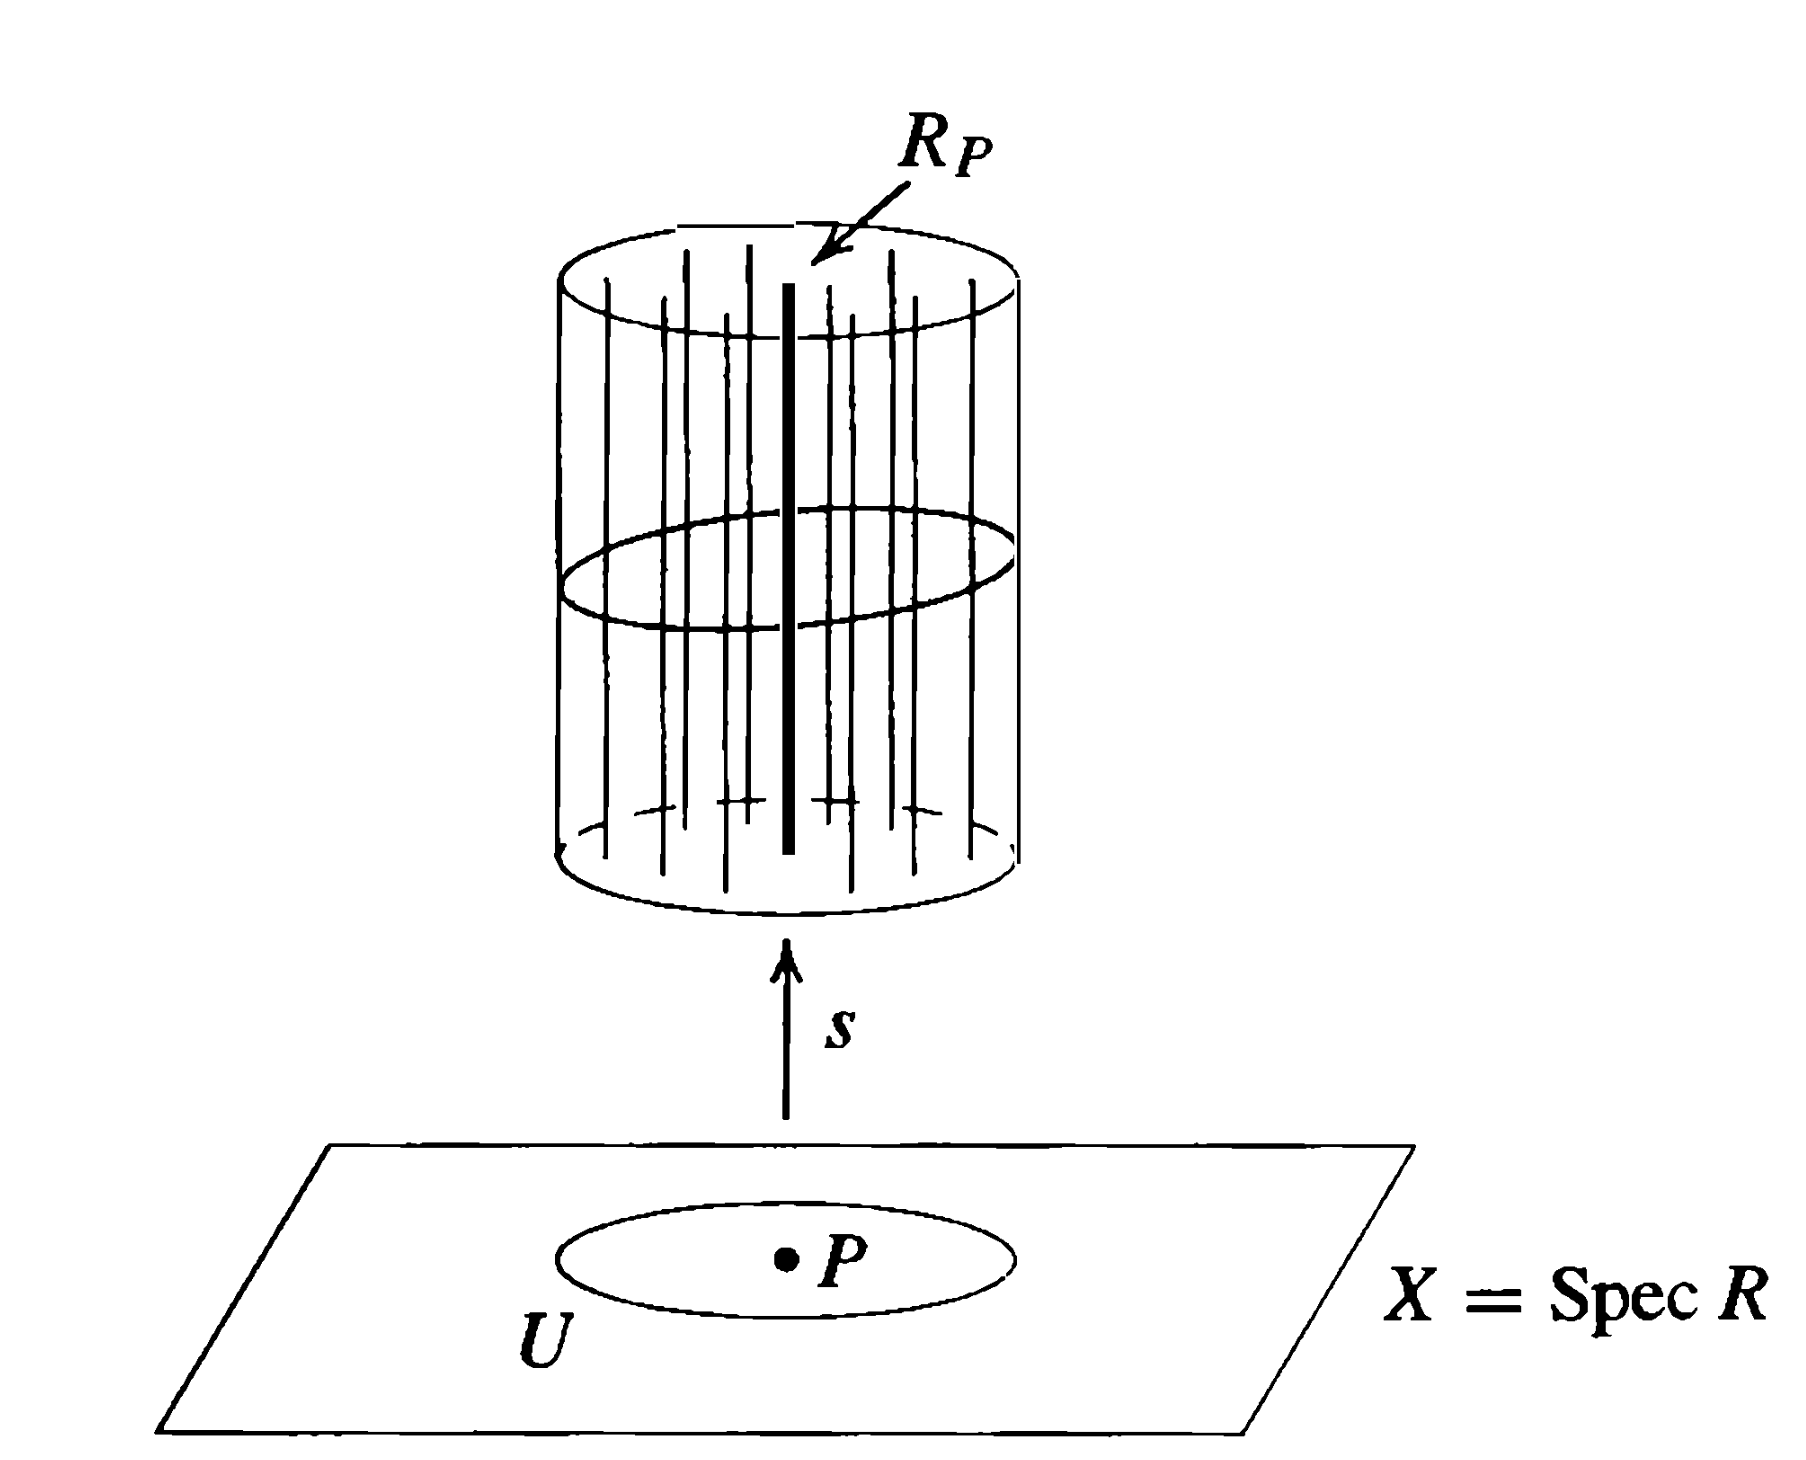
\includegraphics[width=0.6\textwidth]{stalk_analogy.png}
    \caption{Geometric intuition of stalks and sections}
    \label{fig:stalk_analogy}
\end{figure}
\end{itemize}

\subsubsection{Affine Scheme}

\begin{definition}{Affine Scheme}\\
Let $R$ be a ring. The pair $(\text{Spec }R ,\mathcal{O}_{\text{Spec }R})$, consisting of the space $\text{Spec }R$ with the Zariski topology together with the structure sheaf $\mathcal{O}_{\text{Spec }R}$, is called an \textit{affine schemes}.
\end{definition}

\noindent\textbf{Remark:} The notion of affine schemes gives a completely algebraic generalization of the geometry of affine algebraic sets valid for arbitrary rings.

\noindent\textbf{Example:} Now we give some examples of the two notions of structure sheaves and of stalks and hence of the concept of affine scheme:
\begin{itemize}
    \item If $F$ is a field, then $X=\text{Spec }F= \{(0)\}$. In this case, there are only two open sets $X$ and $\emptyset$, both of which are principal open sets: $X=X_1$ and $\emptyset =X_0$. The global sections are $\mathcal{O}(X) =F$. There is only stalk: $\mathcal{O} _{(0)} =F_0=F$.

    \item If $R=\mathbb{Z}$, then $R$ is a PID, so every open set in $X=\text{Spec }\mathbb{Z}$ is principal open:
    \begin{gather*}
    X_n = \{(p) \mid p \nmid n\} \quad \text{and} \\
    \mathcal{O}(X_n) = \mathbb{Z}_n = \mathbb{Z}[1/n] = \{a/b \in \mathbb{Q} \mid \text{if the prime } p \mid b \text{ then } p \mid n\}.
    \end{gather*}
    For nonzero $p$, the stalk at $(p)$ is the local ring $\mathbb{Z}_{(p)}$ and the stalk at $(0)$ is $\mathbb{Q}$. All the restriction maps as well as the maps from sections to stalks are the natural inclusions.

    \item For a general ID $R$ with quotient field $F$, the stalks and sections are
    \begin{gather*}
    \mathcal{O} (U)= \{a/b\in F \mid b\notin P,\forall P\in U\}\\
    \mathcal{O}_P=R_P= \{a/b \in F\mid b\notin P\}
    \end{gather*}
    where the stalk at $(0)$ is $F$, i.e.: $\mathcal{O}_{(0)}= F$. Again, the restriction maps and the maps to the stalks are all inclusions.

    \item For the local ring $R= \mathbb{Z}_{(2)} =\{ a/b\in \mathbb{Q} \mid b\text{ odd} \}$, we have $\text{Spec }R=\{(0) ,(2)\}$ with $(2)$ the only closed point and $\{(0) \}=X_2$ a principal open set. The sections $\mathcal{O} (\{0\})$ are $R_2=\mathbb{Q}$ and the stalks are $\mathcal{O}_{(0)}=R_{(0)} =\mathbb{Q}$ and $\mathcal{O}_{(2)} =R_{(2)} =R$.
\end{itemize}

\noindent\textbf{Intuition:} Now we consider the relationship of the affine schemes corresponding to rings $R$ and $S$ with respect to a ring homomorphism from $R$ to $S$:\\
Suppose that $\varphi:R \to S$ is a ring homomorphism. Then by the Principal Open Sets-Properties Prop.7, there is an induced continuous map $\varphi^*:Y= \text{Spec }S\to X=\text{Spec }R$ and under this map the full preimage of the principal open set $X_g$ for $g\in R$ is the principal open set $Y_{\varphi(g)}$.\\
Also, $\varphi$ induces a map on corresponding sections, as follows: Let $Q' \in Y$ be any element in $\text{Spec }S$ and let $Q= \varphi^*(Q')= \varphi^{-1} (Q') \in X$ be the corresponding element in $\text{Spec }R$. If $U$ is a Zariski open set in $Y$ containing $Q'$. Note that $\varphi$ induces a natural ring homomorphism, say $\varphi_Q$, from the localization $R_Q$ to the localization $S_{Q'}$ defined by
\[
\varphi_Q (a/f) := \varphi(a) /\varphi(f) \in S_{Q'}
\]
for $f\notin Q$. Let $s\in \mathcal{O}_X(U)$ be a section of the structure sheaf of $X$ given locally in the neighborhood $X_g$ of $P\in X$ by $a/g^n$. It is easy to check that the composite
\[
s': U' \overset{\varphi^*}{\longrightarrow} U \overset{s}{\longrightarrow} \bigsqcup_{Q \in U}R_Q \overset{\varphi}{\longrightarrow} \bigsqcup_{Q' \in U'} S_{Q'}
\]
defines a map given locally in the neighborhood $Y_{\varphi(g)}$ by the element $\varphi(g) /\varphi(g)^n$, so that $s'\in \mathcal{O}_Y (U')$ is a section of the structure sheaf of $Y$. It is then straightforward to check that the resulting map $\varphi^\# :\mathcal{O}_{X,P} \to \mathcal{O}_{Y,P'}$ for any point $P' \in \text{Spec }S$ and corresponding point $P= \varphi^* (P') \in \text{Spec }R$. Under the isomorphism in the Stalk-Localization-Isomorphism Prop, the homomorphism $\varphi^\#:R_P \cong \mathcal{O}_{X,P} \to S_{P'} \cong \mathcal{O}_{Y,P'}$ is just the natural ring homomorphism $\varphi_P$ on the localizations induced by the homomorphism $\varphi$. In particular, the inverse image under $\varphi^\#$ of the maximal ideal in the local ring $\mathcal{O}_{Y,P'}$ is the maximal ideal in the local ring $\mathcal{O}_{X,P}$.

\begin{definition}{Morphisms of Affine Schemes}\\
Let $(\text{Spec }R, \mathcal{O}_{\text{Spec }R})$ and $(\text{Spec }S, \mathcal{O}_{\text{Spec }S})$ be two affine schemes. A \textit{morphism of affine schemes} from $(\text{Spec }R, \mathbb{O}_{\text{Spec }R})$ to $(\text{Spec }S ,\mathcal{O}_{\text{Spec } S})$ is a pair $(\varphi^*, \varphi^\#)$ satisfying the following three conditions:
\begin{enumerate}
    \item $\varphi^*: \text{Spec }S \to \text{Spec }R$ is Zariski continuous.
    \item There are ring homomorphisms $\varphi^\#: \mathcal{O} (U) \to \mathcal{O} ((\varphi^*)^{-1} (U))$ for every Zariski open subset $U$ in $\text{Spec }R$ that commute with the restriction maps.
    \item If $P'\in \text{Spec }S$ with corresponding point $P= \varphi^\# (P') \in \text{Spec }R$, then under the induced homomorphism on stalks $\varphi^\# :\mathcal{O}_{\text{Spec }R,P} \to \mathcal{O}_{\text{Spec }S,P'}$, the preimage of the maximal ideal of $\mathcal{O}_{\text{Spec }S,P'}$ is the maximal ideal of $\mathcal{O} _{\text{Spec }R,P}$.
\end{enumerate}
\end{definition}

\noindent\textbf{Remark:} A homomorphism $\psi: A\to B$ between the local rings with the property that the preimage of the maximal ideal of $B$ is the maximal ideal of $A$ is called a \textit{local homomorphism} of local rings. The third condition in the definition is then the statement that the induced homomorphism on stalks is required to be a local homomorphism.

\begin{theorem}{Equivalence-of-Categories-between-Affine Schemes-and0Rings Theorem}\\
Every ring homomorphism $\varphi: R\to S$ induces a morphism
\[
(\varphi^* ,\varphi^\#): (\text{Spec }S, \mathcal{O}_{\text{Spec }S}) \to (\text{Spec }R ,\mathcal{O}_{\text{Spec }R})
\]
of affine schemes. Conversely, every morphism of affine schemes arises from such a ring homomorphism $\varphi$.
\end{theorem}

% ------------- 请将以下代码插入到你的章节文件 (如 chapter 1.tex) 中 -------------

\begin{theorem}[Equivalence of Rings and Affine Schemes, Theorem 59]
Every ring homomorphism $\varphi: R \to S$ induces a morphism 
\[
(\varphi^*, \varphi^\#) : (\text{Spec } S, \mathcal{O}_{\text{Spec } S}) \to (\text{Spec } R, \mathcal{O}_{\text{Spec } R})
\]
of affine schemes. Conversely, every morphism of affine schemes arises from such a ring homomorphism $\varphi$.
\end{theorem}

\begin{proof}
The proof consists of two directions. The fact that a ring homomorphism induces a morphism of affine schemes was already shown in the preceding discussion. We focus on thoroughly proving the converse: extracting a ring homomorphism from a morphism of affine schemes and showing they are naturally equivalent.

\textbf{Step 1: Extracting the global ring homomorphism $\varphi: R \to S$.} \\
Suppose we are given a morphism of affine schemes, denoted by $(f, f^\#) : (\text{Spec } S, \mathcal{O}_{\text{Spec } S}) \to (\text{Spec } R, \mathcal{O}_{\text{Spec } R})$. (Note: we use $f$ for the continuous map to avoid confusion with the $\varphi$ we are trying to construct). \\
By the definition of a morphism of ringed spaces, $f^\#$ is a morphism of sheaves from $\mathcal{O}_{\text{Spec } R}$ to the pushforward sheaf $f_* \mathcal{O}_{\text{Spec } S}$. 
Evaluating these sheaves on the global topological space $U = \text{Spec } R$, we get a ring homomorphism on the global sections:
\[
f^\#(\text{Spec } R) : \mathcal{O}_{\text{Spec } R}(\text{Spec } R) \to (f_* \mathcal{O}_{\text{Spec } S})(\text{Spec } R).
\]
By the definition of the pushforward sheaf, $(f_* \mathcal{O}_{\text{Spec } S})(\text{Spec } R) = \mathcal{O}_{\text{Spec } S}(f^{-1}(\text{Spec } R)) = \mathcal{O}_{\text{Spec } S}(\text{Spec } S)$. \\
By Proposition 57 (the structure sheaf evaluated on the whole spectrum recovers the original ring), we have natural ring isomorphisms:
\[
\mathcal{O}_{\text{Spec } R}(\text{Spec } R) \cong R \quad \text{and} \quad \mathcal{O}_{\text{Spec } S}(\text{Spec } S) \cong S.
\]
Composing $f^\#(\text{Spec } R)$ with these isomorphisms gives us a well-defined ring homomorphism between the underlying rings:
\[
\varphi : R \to S.
\]

\textbf{Step 2: Checking the local behavior on stalks (The Commutative Diagram).} \\
Pick any prime ideal $P' \in \text{Spec } S$. Let its image under the continuous map be $P = f(P') \in \text{Spec } R$. \\
Because $(f, f^\#)$ is a morphism of \textit{locally ringed spaces} (which affine schemes are), $f^\#$ induces a \textbf{local homomorphism} on the stalks at $P'$. 
By Proposition 58, the stalk of $\mathcal{O}_{\text{Spec } R}$ at $P$ is the localization $R_P$, and the stalk of $\mathcal{O}_{\text{Spec } S}$ at $P'$ is $S_{P'}$. Thus, we have a local ring homomorphism:
\[
\varphi^\#_{P'} : R_P \to S_{P'}.
\]
Because the sheaf morphism $f^\#$ is compatible with the restriction maps (going from global sections to local stalks), the following diagram must commute:
\[
\begin{tikzcd}[row sep=large, column sep=large]
R \arrow[r, "\varphi"] \arrow[d, "\text{nat}"'] & S \arrow[d, "\text{nat}"] \\
R_P \arrow[r, "\varphi^\#_{P'}"'] & S_{P'}
\end{tikzcd}
\]
where the two vertical maps are the natural localization homomorphisms (e.g., $r \mapsto r/1$).

\textbf{Step 3: Proving the topological map $f$ is exactly $\varphi^*$.} \\
We need to show that the given continuous map $f(P')$ is exactly the pullback of prime ideals under our constructed $\varphi$, i.e., $f(P') = \varphi^{-1}(P')$. \\
Recall that a local ring homomorphism (like $\varphi^\#_{P'}$) must map the unique maximal ideal of the domain into the unique maximal ideal of the codomain. 
\begin{itemize}
    \item The unique maximal ideal of the local ring $R_P$ is $P R_P$.
    \item The unique maximal ideal of the local ring $S_{P'}$ is $P' S_{P'}$.
\end{itemize}
Therefore, taking the pre-image under $\varphi^\#_{P'}$, we have:
\[
(\varphi^\#_{P'})^{-1}(P' S_{P'}) = P R_P.
\]
Now, let's trace this equality back up through the commutative diagram to the global rings $R$ and $S$.
If we pull back $P' S_{P'}$ along the natural map $S \to S_{P'}$, we get the original prime ideal $P'$ in $S$. Pulling this further back to $R$ via $\varphi$ gives $\varphi^{-1}(P')$.
On the other hand, going the other way around the diagram, pulling back $P R_P$ along the natural map $R \to R_P$ recovers $P$ (since $P$ is prime).
Because the diagram commutes, the results of pulling back through both paths must be identical. Hence:
\[
\varphi^{-1}(P') = P.
\]
Since we initially defined $P = f(P')$, this proves $f(P') = \varphi^{-1}(P')$. By definition, $\varphi^{-1}(P')$ is exactly $\varphi^*(P')$. So the continuous map $f$ is identical to $\varphi^*$.

\textbf{Step 4: Conclusion.} \\
We have shown that $f = \varphi^*$. Because the structural sheaf morphism $f^\#$ on affine schemes is entirely determined by its action on the global sections (which we defined as $\varphi$) and its compatibility with localizations, it follows that $f^\#$ is exactly the induced sheaf morphism $\varphi^\#$. \\
Consequently, the arbitrary morphism $(f, f^\#)$ we started with is precisely $(\varphi^*, \varphi^\#)$, meaning every morphism of affine schemes is uniquely induced by a ring homomorphism.
\end{proof}